\documentclass[10pt, landscape]{article}
\usepackage[scaled=0.92]{helvet}
\usepackage{multicol}
\usepackage{calc}
\usepackage{ifthen}
\usepackage[landscape]{geometry}
%\usepackage{hyperref}

\usepackage{newtxtext} 

%for strikeout
\usepackage{ulem}

%For editing parbox
\usepackage[table]{xcolor}
%For editing itemise margins, reduce iterm separaion and list separation
\usepackage{enumitem}
% For math
\usepackage{amsmath,amsthm,amsfonts,amssymb}

%For pictures / figures
\usepackage{color,graphicx,overpic}
\graphicspath{ {./images/} }

%\usepackage{newtxtext} 
%\usepackage{amssymb}
%\usepackage[table]{xcolor}
%\usepackage{vwcol}
%\usepackage{tikz}
%\usepackage{wrapfig}
%\usepackage{makecell}

\pdfinfo{
  /Title (CS2107-notes.pdf)
  /Creator (Ger Teck)
  /Author (Ger Teck)
  /Subject ()
  /Keywords (tex)}

%% Margins for PAPER

% This sets page margins to .5 inch if using letter paper, and to 1cm
% if using A4 paper. (This probably isn't strictly necessary.)
% If using another size paper, use default 1cm margins.
\ifthenelse{\lengthtest { \paperwidth = 11in}}
	{ \geometry{top=.3in,left=.3in,right=.3in,bottom=.3in} }
	{\ifthenelse{ \lengthtest{ \paperwidth = 297mm}}
		{\geometry{top=0.5cm,left=0.5cm,right=0.5cm,bottom=0.5cm} }
		{\geometry{top=0.5cm,left=0.5cm,right=0.5cm,bottom=0.5cm} }
	}

% Turn off header and footer
\pagestyle{empty}
% for tight centres (less spacing)
\newenvironment{tightcenter}{%
  \setlength\topsep{0.5pt}
  \setlength\parskip{0.5pt}
  \begin{center}
}{%
  \end{center}
}

% Redefine section commands to use less space
\makeatletter
\renewcommand{\section}{\@startsection{section}{1}{0mm}%
                                {-1ex plus -.5ex minus -.2ex}%
                                {0.5ex plus .2ex}%x
                                {\normalfont\large\bfseries}}
\renewcommand{\subsection}{\@startsection{subsection}{2}{0mm}%
                                {-1explus -.5ex minus -.2ex}%
                                {0.5ex plus .2ex}%
                                {\normalfont\normalsize\bfseries}}
\renewcommand{\subsubsection}{\@startsection{subsubsection}{3}{0mm}%
                                {-1ex plus -.5ex minus -.2ex}%
                                {1ex plus .2ex}%
                                {\normalfont\small\bfseries}}
% change font
%\renewcommand{\familydefault}{\sfdefault}
%\renewcommand\rmdefault{\sfdefault}
\linespread{1.05}

\makeatother

% Define BibTeX command
\def\BibTeX{{\rm B\kern-.05em{\sc i\kern-.025em b}\kern-.08em
    T\kern-.1667em\lower.7ex\hbox{E}\kern-.125emX}}

% Don't print section numbers
\setcounter{secnumdepth}{0}

\setlength{\parindent}{0pt}
\setlength{\parskip}{0pt plus 0.5ex}

%% this changes all items (enumerate and itemize, reduce margins) ITEMIZE SEPARATION HERE
\setlength{\leftmargini}{0.5cm}
\setlength{\leftmarginii}{0.5cm}
\setlist[itemize,1]{leftmargin=2mm,labelindent=1mm,labelsep=1mm, itemsep = 0mm}
\setlist[itemize,2]{leftmargin=4mm,labelindent=1mm,labelsep=1mm, itemsep = 0mm}

%itemsep = 0mm
%\setlist{nosep}

% -------------------------------------------------------------------------------

% START OF DOCUMENT HERE

\begin{document}
\raggedright
\footnotesize
\begin{multicols*}{3}

% multicol parameters
% These lengths are set only within the two main columns
%\setlength{\columnseprule}{0.25pt}
\setlength{\premulticols}{1pt}
\setlength{\postmulticols}{1pt}
\setlength{\multicolsep}{1pt}
\setlength{\columnsep}{2pt}

%% TODO COMMENT OUT
\iffalse

%% DOCUMENT NAME HERE
\begin{center}
     \Large{\textbf{CS2107 Introduction to \\
     				 Information Security}} \\
\end{center}
AY23/24 Sem 2, github.com/gerteck


\section{0. Introduction}
CS2107: Introductory module, illustrates fundamentals of how systems fail due to malicious activities and how they can be protected. 

\textbf{Lecture Notes notation}
\begin{itemize}
\item \textbf{Textbook:} Security in Computing (5th ed). Prentice Hall. Reference [PFx.y] refer to chapter x section y of this book.
\item Links with ``read'': Part of lecture, required. 
\item Links with ``see'': Optional good to browse references.
\end{itemize}

\subsection{Internet Security Threat Report Exc. Summary}
Persistent threats are threats that often operate within the shadows, outside of attention focused. 
\begin{itemize}
\item Highly targeted, often use combination of social engineering and software vulnerabilities to establish footholds within the targeted enterprise.
\item Network protection not enough to mitigate threats, comprehensive monitoring program required to scan all internal and external network traffic. Identifying, securing data is also key to protecting assets.
\item Recent attack types: Formjacking, Ransomware, Living off the Land (LotL), 
\end{itemize}


\subsection{Introduction to Computer/Info Security}
Systems may fail due to operator mistakes, hardware failures, poor implementation etc. Many systems robust against typical noise. Security is about intentional failures inflicted by deliberate human actions. \\
\textbf{Security Definitions:} C-I-A triad
\begin{itemize}
\item \textbf{Confidentiality}: Prevention of unauthorized disclosure of information.
\item \textbf{Integrity}: Prevention of unauthorized modification of info / processes.
\item \textbf{Availability}: Prevention of unauthorized withholding of info / resources.
\item Other requirements may include (Confidentiality: anonymity, covert channel), (Integrity: Non-repudiation (digital signature)), (Other: Accountability, traitor-tracing (printout w hidden watermark)) etc.
\item Importance of understanding security requirements before adopting mechanisms. Do not adopt mismatched protection mechanisms.
\end{itemize}

\subsubsection{Difficulties in achieving Security}
\begin{itemize}
\item \textbf{Security not considered} (in early design stage). \\
Lack of adversarial thinking in design / trade-off in security with ease-of-use, performance / cost.
\item Difficult to formulate requirements /design / implementation bugs. 
\item Difficult to operate/manage (Human error). \\
\item \textbf{Known Vulnerabilities: CVE (Common vulnerabilities \& Exposures}. Repository of discovered vulnerabilities. Significant portion considered "implementation bugs".
\item \textbf{Zero-day Vulnerabilities}: Unpublished vulnerabilities. If attackers deploy attacks on zero-day v., victims have "zero-day" to react. Not easy to get.
\end{itemize} 


\section{1. Encryption}

% To update:
\textbf{Key Summary \& Takeaways}
\begin{itemize}
\item \textbf{Encryption designed for confidentiality.} (Not necessarily integrity).
\item Formulate attack scenario by defining attacks it can prevent. 
\item Notions of "Oracle": Encryption, Decryption, Padding Oracle.
\item \textbf{Key strength}: Quantifying security by equivalence of best-known attack to exhaustive search.
\item No known efficient attacks on modern schemes under "original" threat models, but there are pitfalls. Such as implementation error (wrong mode, wrong random source, mishandle of IV), side channel attack, implicity require integrity, padding oracle attack.
\item Design of various symmetric key encryption schemes:
	\begin{itemize}
	\item One-time pad, stream cipher (xor'ing with "pseudo-random" string)
	\item Block cipher (mode of operations: CBC, ECB, CTR, GCM)
	\end{itemize}
\item \textbf{Crucial role of IV}. (Need randomness for indistinguishability). Make encryption probabilistic, how it is deployed, why it is important.
\end{itemize}

\subsubsection{Definitions}
\begin{itemize}
\item \textbf{Symmetric Key Encryption Scheme}: Two algorithms: encryption and decryption. Meets correctness property, and must be secure.
\item \textbf{Correctness:} $(D_k (E_k (x) ) = x )$. \textbf{Security}: Informally, "difficult" to derive useful info of the key k, and plaintext x. Ciphertext resemble random sequence of bytes.
\item \textbf{Cryptography}: Study of techniques in securing communication in present of adversaries with access. Encryption just a primitive (other includes crypto hash, digital signature etc. Common placeholders: Alice, Bob, Eve ("eavesdroppper"), Mallory (malicious, modify message), etc.
\end{itemize}

\subsubsection{Attack Model}
\textit{Aka: Threat / Adversary / Security Model, Attack Scenario.} \\
Measuring \textbf{security of a system}: Through attack classes it can prevent. Secure w.r.t these classes of attacks. Attack models are application-dependent. Attack models described by:
\begin{itemize}
\item Attacker's knowledge (info / service exposed) and computing resources
\item Attacker's goal
\end{itemize}
\textbf{Types of information we assume access to:} (Access to info can be formulated to accesses to an \textbf{"Oracle"}).
\begin{itemize}
\item \textbf{Ciphertext only attack:} Adversary given collection of ciphertext c. May know some properties 
of the plaintext, for e.g. the plaintext is an English sentence. (adv. can’t choose plaintext).
\item \textbf{Known plaintext attack:} Adversary given collection of plaintext m and corresponding ciphertext c. (adv. can’t choose plaintext.)
\item \textbf{Chosen plaintext attack (CPA):} Access to blackbox (i.e. the oracle). \\
Can choose, feed any plaintext m, obtain corresponding ciphertext c (all encrypt with the same key), reasonable large number of times. Can see ciphertext and choose next input.  \textit{(black-box called encryption oracle).}
\item \textbf{Chosen ciphertext attack (CCA2)}: Same as chosen plaintext attack, but adv. chooses ciphertext and blackbox outputs plaintext. \textit{black-box called decryption oracle}. \\
\textbf{Note}: (strange to assume attacker has power to decrypt, but good reason is that in some practical scenario, attacker does have some but not full decryption capability, e.g. \textit{padding oracle}. To cater for all scenarios, in formulation and design of encryption, we consider oracle with full decryption capability.)
\end{itemize}

\subsubsection{Adversary's Goals}
\begin{itemize}
\item \textbf{Total Break}: Attacker wants to find the key.
\item \textbf{Partial Break}: Few definitions, e.g. decrypt ciphertext, determine coarse information about plaintext, etc.
\item \textbf{Indistinguishability (IND)}: ) Attacker may satisfy with distinguishability of ciphertext: with some “non-negligible” probability more than ½, the attacker is able to distinguish the ciphertexts of a given plaintext (say, “Y”) from the ciphertext of another given plaintext (say, “N”). (Equivalently, unable to distinguish the ciphertext and a randomly sequence).
\item \textbf{Note}: total break most difficult goal, since achieves all. Distinguishability weakest goal, design cryptosystem preventing weakest goal.
\end{itemize}

\section{1.1 Classicial Ciphers (Symmetric)}

\subsection{1.1.1 Substitution Cipher}
\begin{itemize}
\item \textbf{Plaintext, ciphertext}: String over a set of symbols U.
\item \textbf{Key}: Subsitution table S, 1-1 onto function from U to U.
\item \textbf{Key space}: Set of all possible keys (e.g. 27). \textbf{Space Size} is total number of possible keys (factorial, 27!). \textbf{Key Size} is number of bits required to represent a key. (log 2 (27!), since 27! unique) 
\item \textbf{Exhaustive Search (Brute-force): Can be infeasible in worst case}
\item \textbf{Known-plaintext-attack}: Access to pairs of ciphertext and corresponding plaintexts: \textit{Sub. cipher “not secure / totally broken under known plaintext attack”}. (Possible in practice, e.g. certain words in header of email "From, Subject", protocols bytes fixed header information etc.)
\item \textbf{Ciphertext only attack}: Vulnerable to frequency analysis attack, when plaintexts English sentences.
\end{itemize}

\subsection{1.1.2 Permutation Cipher (aka transposition cipher)}
\begin{itemize}
\item Groups plaintext into blocks of $t$ characters, applies secret permutation (1-1 onto function). Fails miserably on known-plaintext attack.
\centerline{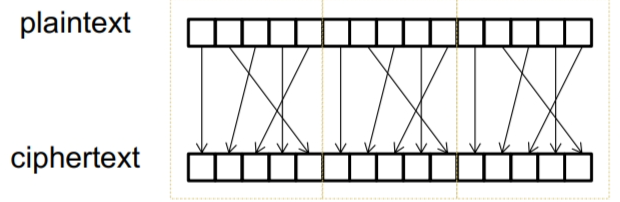
\includegraphics[width=0.4\linewidth]{permutationCipher}}
\end{itemize}

\begin{itemize}
\item S \& P cipher not secure, performing substitution multiple times no use. However, by interlacing them (S\&P), attacks become more difficult. Many modern encryption scheme (e.g. AES) designed using rounds of S \& P.
\end{itemize}

\subsection{Terminology}
\begin{itemize}
\item \textbf{Cryptosystem}: A system for encryption and decryption.
\item \textbf{Plaintext}: Original form of message.
\item \textbf{Ciphertext}: Encrypted form of message.
\item \textbf{Perfect Secrecy}: A cryptosystem has perfect secrecy if for any distribution $X$, for all $x, y$:
\centerline{$Pr ( X=x | Y=y ) = Pr (X =x) $}.
\item For any ciphertext $y$ and plaintext $x$, the chances attacker correctly predicts x before knowing y, and after knowing y, are the 
same.
\item \textbf{Work Factor}: Difficulty of breaking an encryption (Amount of effort necessary). \\
- (E.g. determine time it would take to test single password, multiply by total possible passwords).
\end{itemize}

\null \null \null \null


\columnbreak

\subsection{1.1.3 One Time Pad}
One-time pad (OTP) is an encryption technique that requires the use of a single-use pre-shared key that is larger than or equal to the size of the message being sent. 
\begin{itemize}
\item Plaintext is paired with a random secret key (known as one-time pad). 
\item Each bit or character of the plaintext encrypted by combining it with corresponding bit/character from pad using modular addition.[1]
\end{itemize}
\centerline{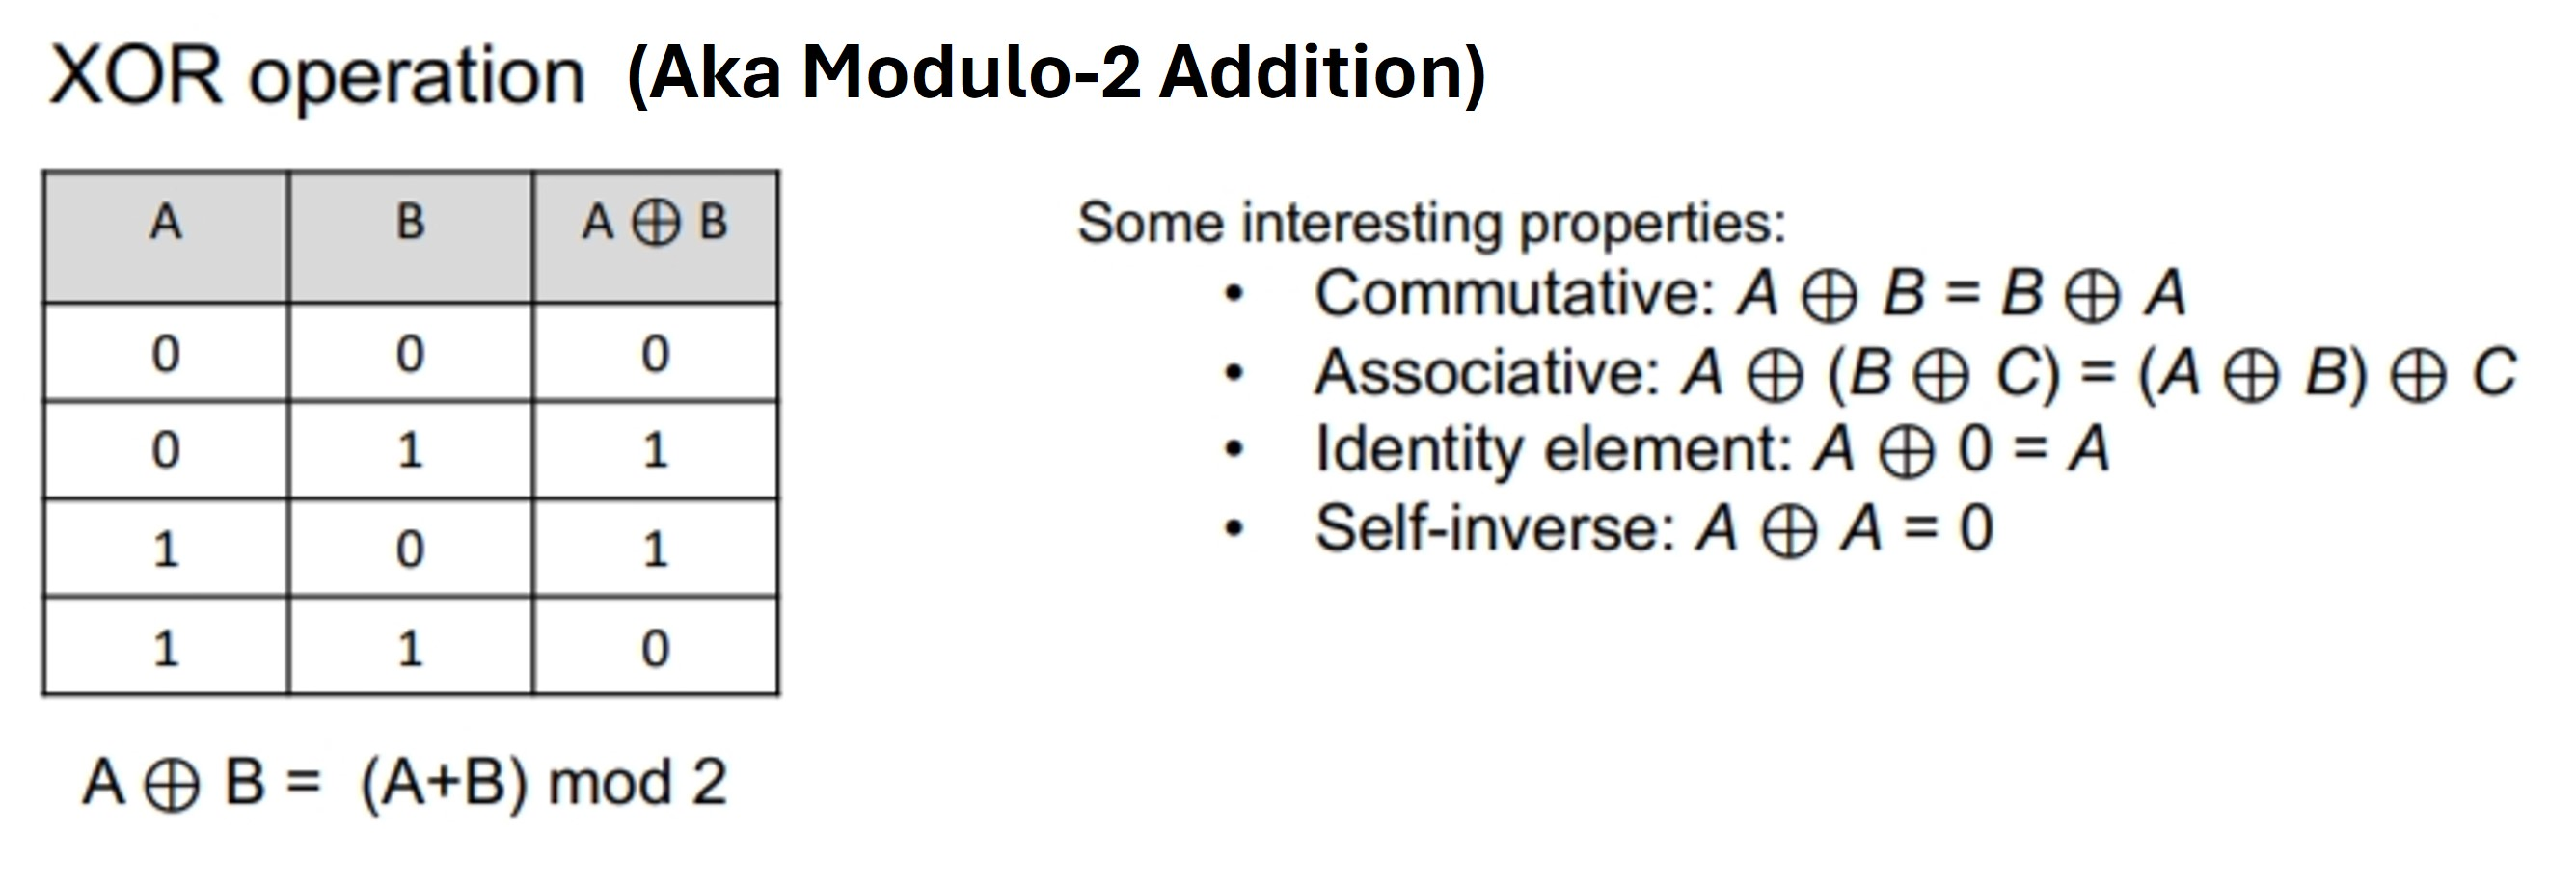
\includegraphics[width=0.4\linewidth]{XOR}}
\centerline{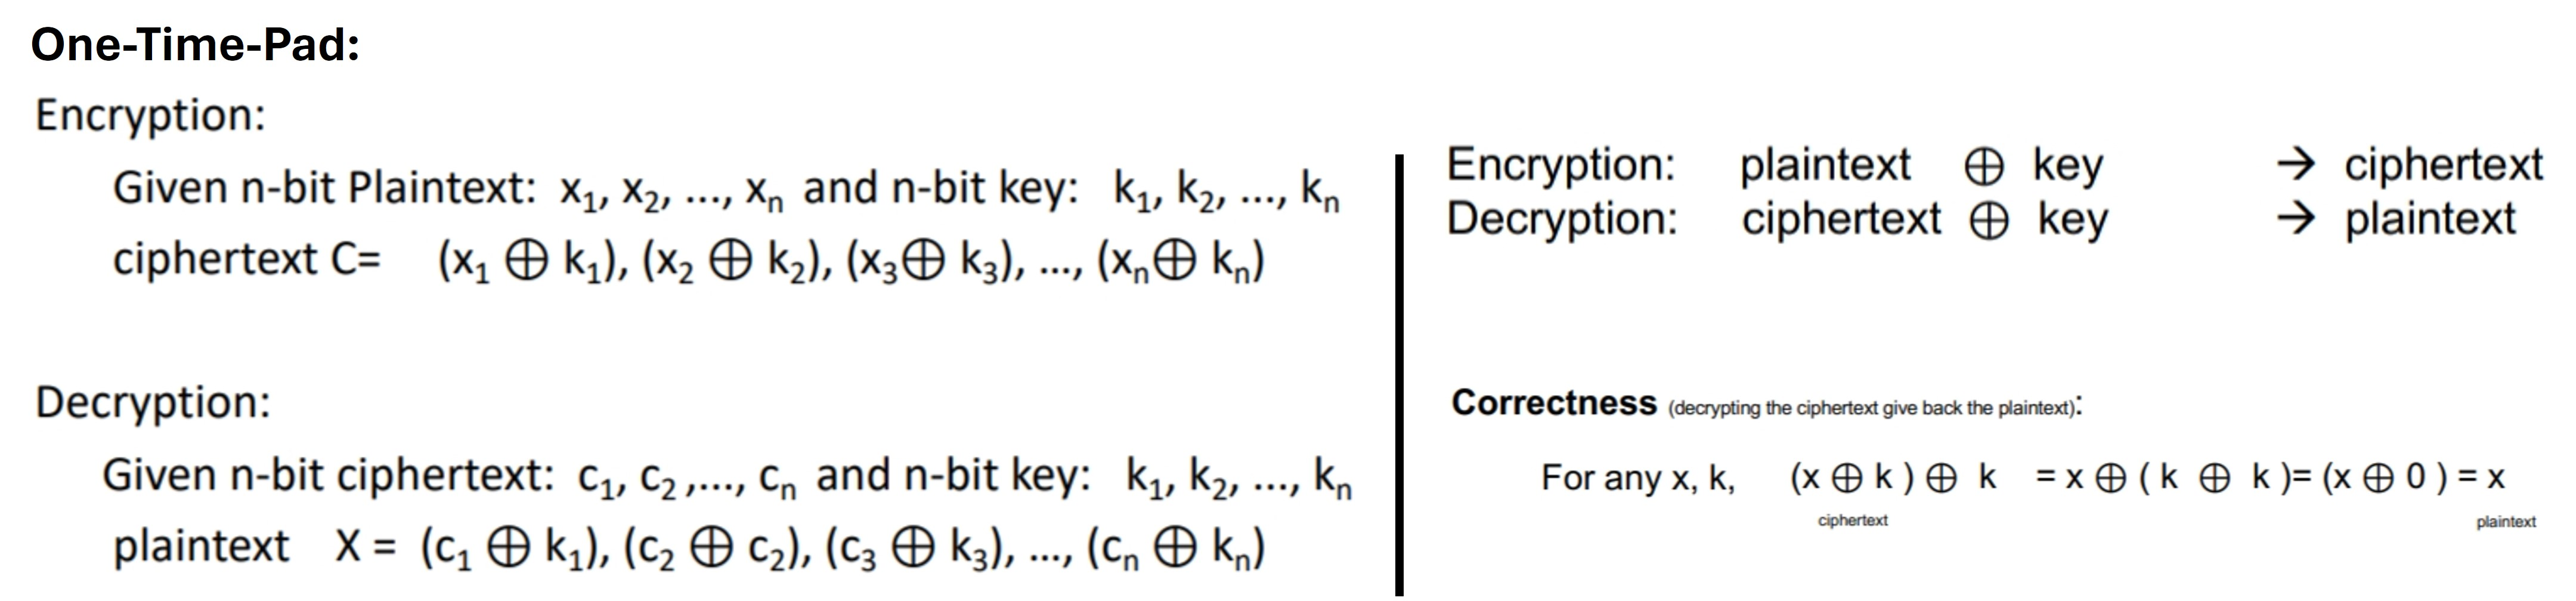
\includegraphics[width=1\linewidth]{OTP}}
\begin{itemize}
\item \textbf{Requirement}: Key cannot be re-used, used only once. Hence, 1GB plaintext would need 1GB key to encrypt.
\item From pair of ciphertext \& plaintext, key can be derived. However, key useless, as only used once.
\item \textbf{Security}: OTP leaks no information of plaintext, sometimes called "unbreakable". There is a exhaustive key for any English sentence. (Perfect Secrecy)
\end{itemize}

\section{1.2 Modern Ciphers (Symmetric)}
Generally refers to schemes that use computer to encrypt / decrypt. E.g:
\\ - DES [Data Encryption Standard 1977] 
\\ - RC4 [Rivest's Cipher 4 1987]
\\ - A5/1 [used in GSM 1987]: Used in WEP Wifi 1999, switched to WPA2
\\ - AES [Adv. Encrypt. Std.], RSA).
\begin{itemize}
\item Designs take into consideration of known-plaintext-attack, freq. analysis and other known attacks.
\item Supposed to be secure, so any successful attack does not perform noticeably better than exhaustive search.
\end{itemize}

\subsection{Key Length, Exhaustive Search DES, AES}
\begin{itemize}
\item \textbf{Security of Encryption Scheme}: Quantified by \textbf{length of key}, w.r.t. exhaustive search.
\item Given a key length of 32 bits, there are $2^{32}$ possible keys. Hence, exhaustive search needs to ``loop'' $2^{32}$ in worst case. 
\item \textbf{No. of bits to be considered ``secure''}: 128, 192, 256 bits, \\
- (NIST recommendation for AES).
\end{itemize}

\subsection{1.2.1 DES, AES and Exhaustive Search}
\begin{itemize}
\item \textbf{Exhaustive Search on DES}: Key length of DES is 56 bits. Previously, seemed infeasible, but has since become easily broken.
\item \textbf{AES}: New standard for block cipher in 2000, AES block length is 127, key length can be 128, 192 or 256 bits. 
\item Currently, no known attacks on AES. NSA classifies AES as ``Suite B Cryptography''.
\end{itemize}

\subsection{1.2.2 Block Cipher \& Mode-of-Operations}
\begin{itemize}
\item \textbf{Block Cipher}: DES \& AES known as ``Block Cipher''. Block cipher designed for some fixed size input/output. \\
- E.g. AES designed for 128 bits input/output.
\item \textbf{Block Cipher Mode Of Operation}: Describes how to repeatedly apply cipher's single block operation to securely transform amounts of data larger than a block. (Extending encryptino from single block to multiple blocks).
\end{itemize}
\centerline{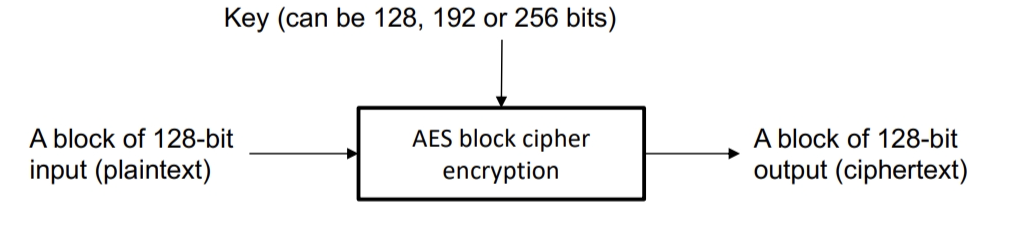
\includegraphics[width=0.8\linewidth]{AES}}

\subsubsection{Mode-of-Operation: ECB Mode on AES}
\begin{itemize}
\item \textbf{Electronic Book Code}: Divide plaintext into blocks, apply block cipher to each block, with the same key.
\item ECB leaks information! AES encryption deterministic without randomly chosen IV.
\item \textbf{Deterministic}: Produces same ciphertext for given plaintext and key over separate executions.
\end{itemize}
\centerline{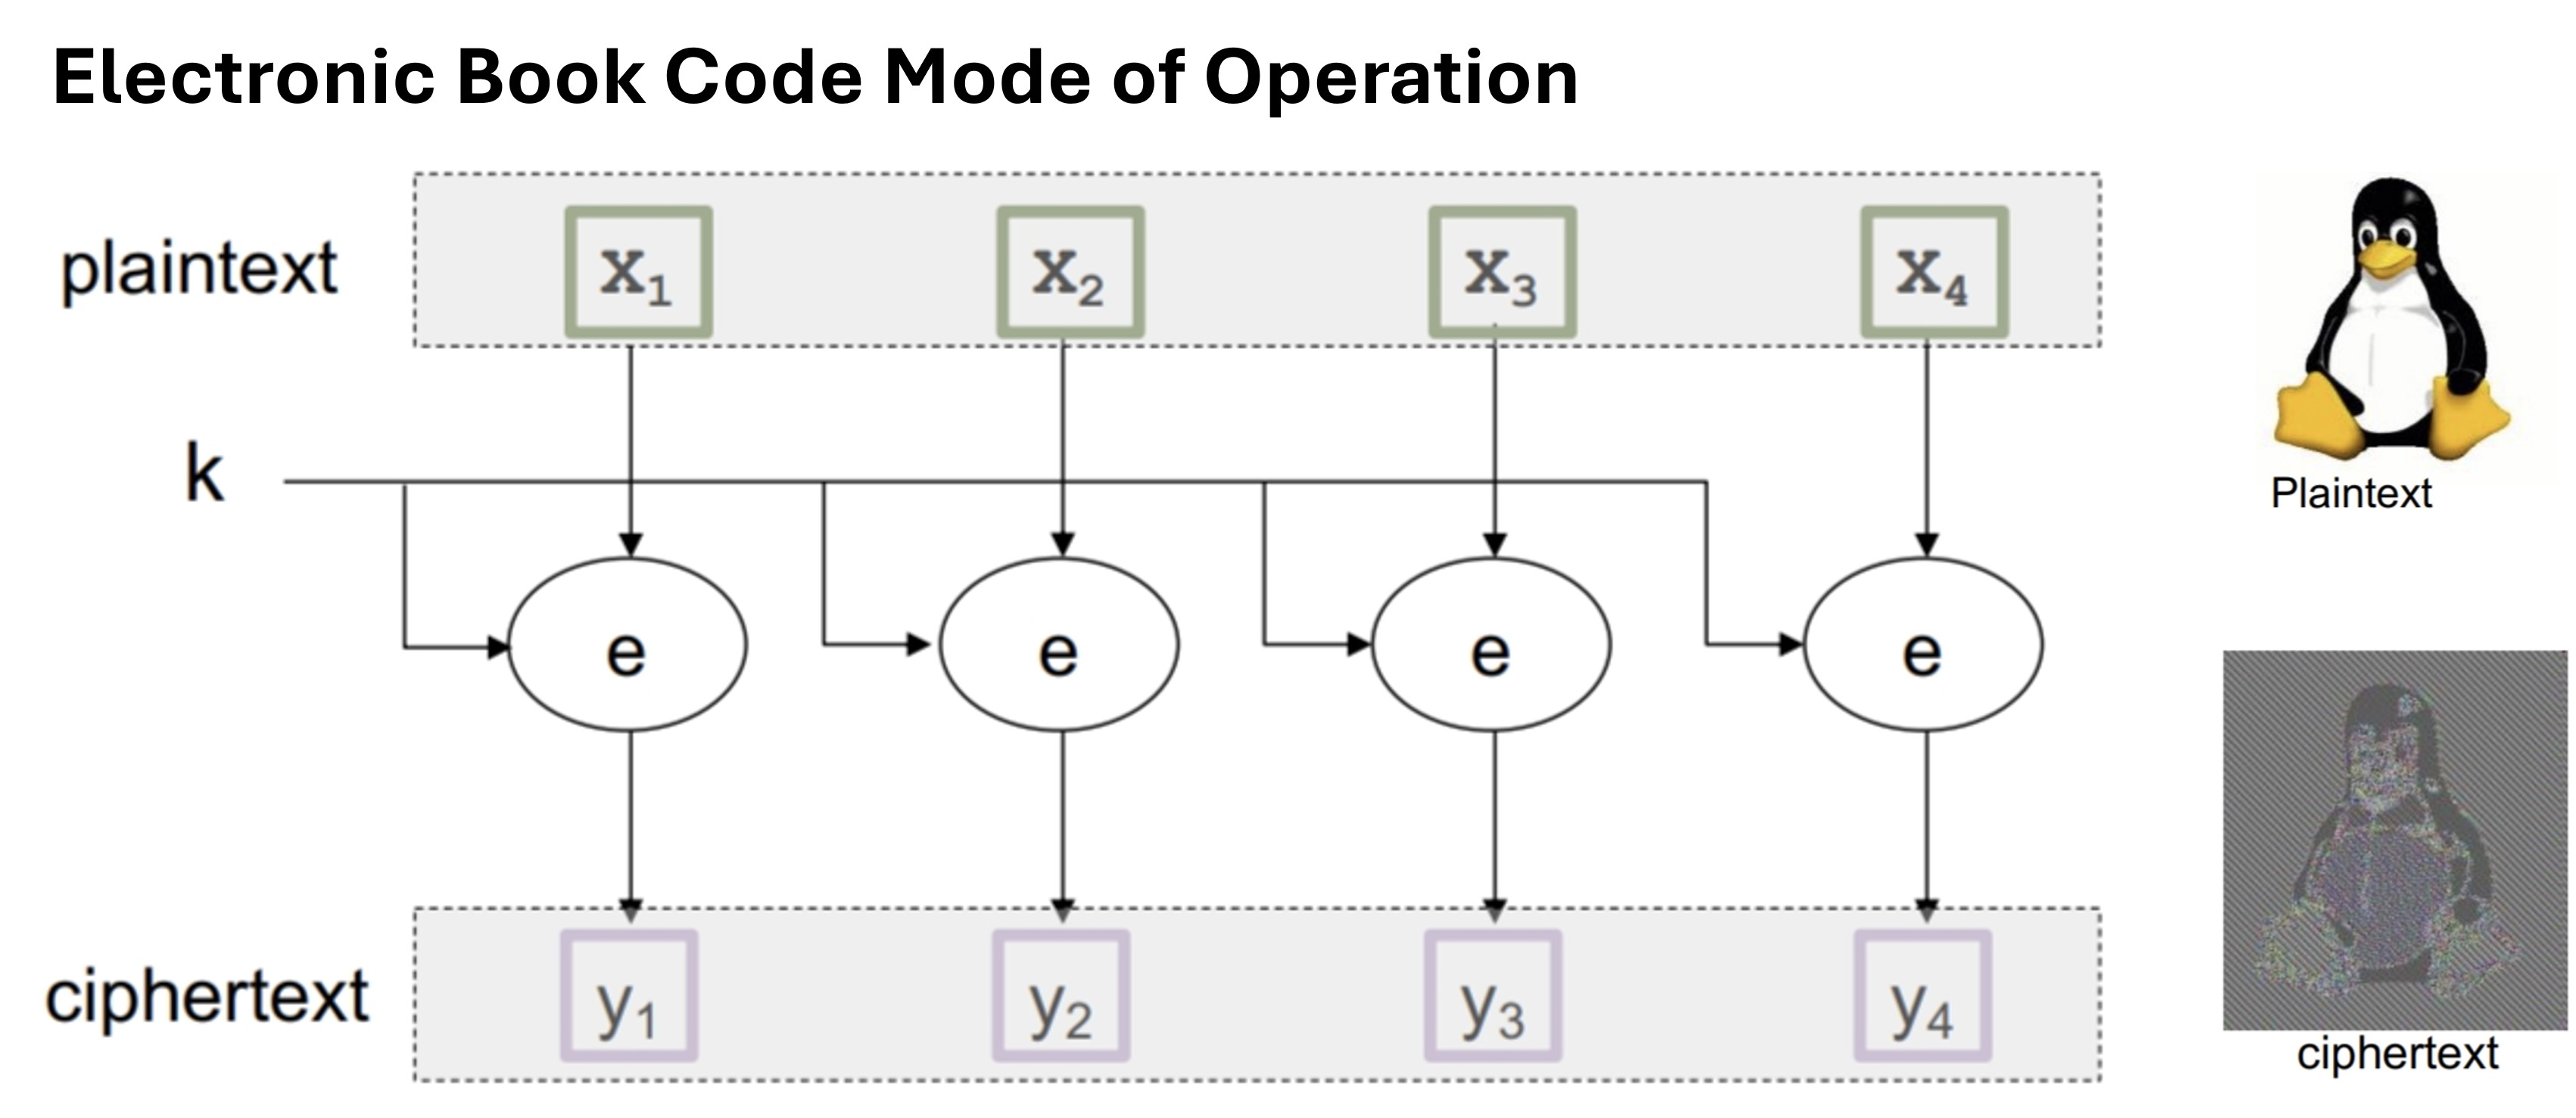
\includegraphics[width=0.7\linewidth]{ECB}}

\subsubsection{Mode-of-Operation: CBC Mode on AES}
\begin{itemize}
\item \textbf{Cipher Block Chaining on AES}: Using an IV, uses chaining process that causes decryption of block of ciphertext to depend on all preceding ciphertext blocks.
\item \textbf{Initialization Vector (IV)}: Arbitrary number of certain length used with secret key, to provide the initial state, for data encryption.
\item \textbf{Encryption}: Each plaintext block is XOR-ed with previous ciphertext block, and then encrypted. Process repeats until all plaintext is ciphertext blocks.
\item \textbf{Decryption}: Reverse encryption process. Note, process does not need to start with final block, can happen simultaneously as all inputs present.
\end{itemize}
\centerline{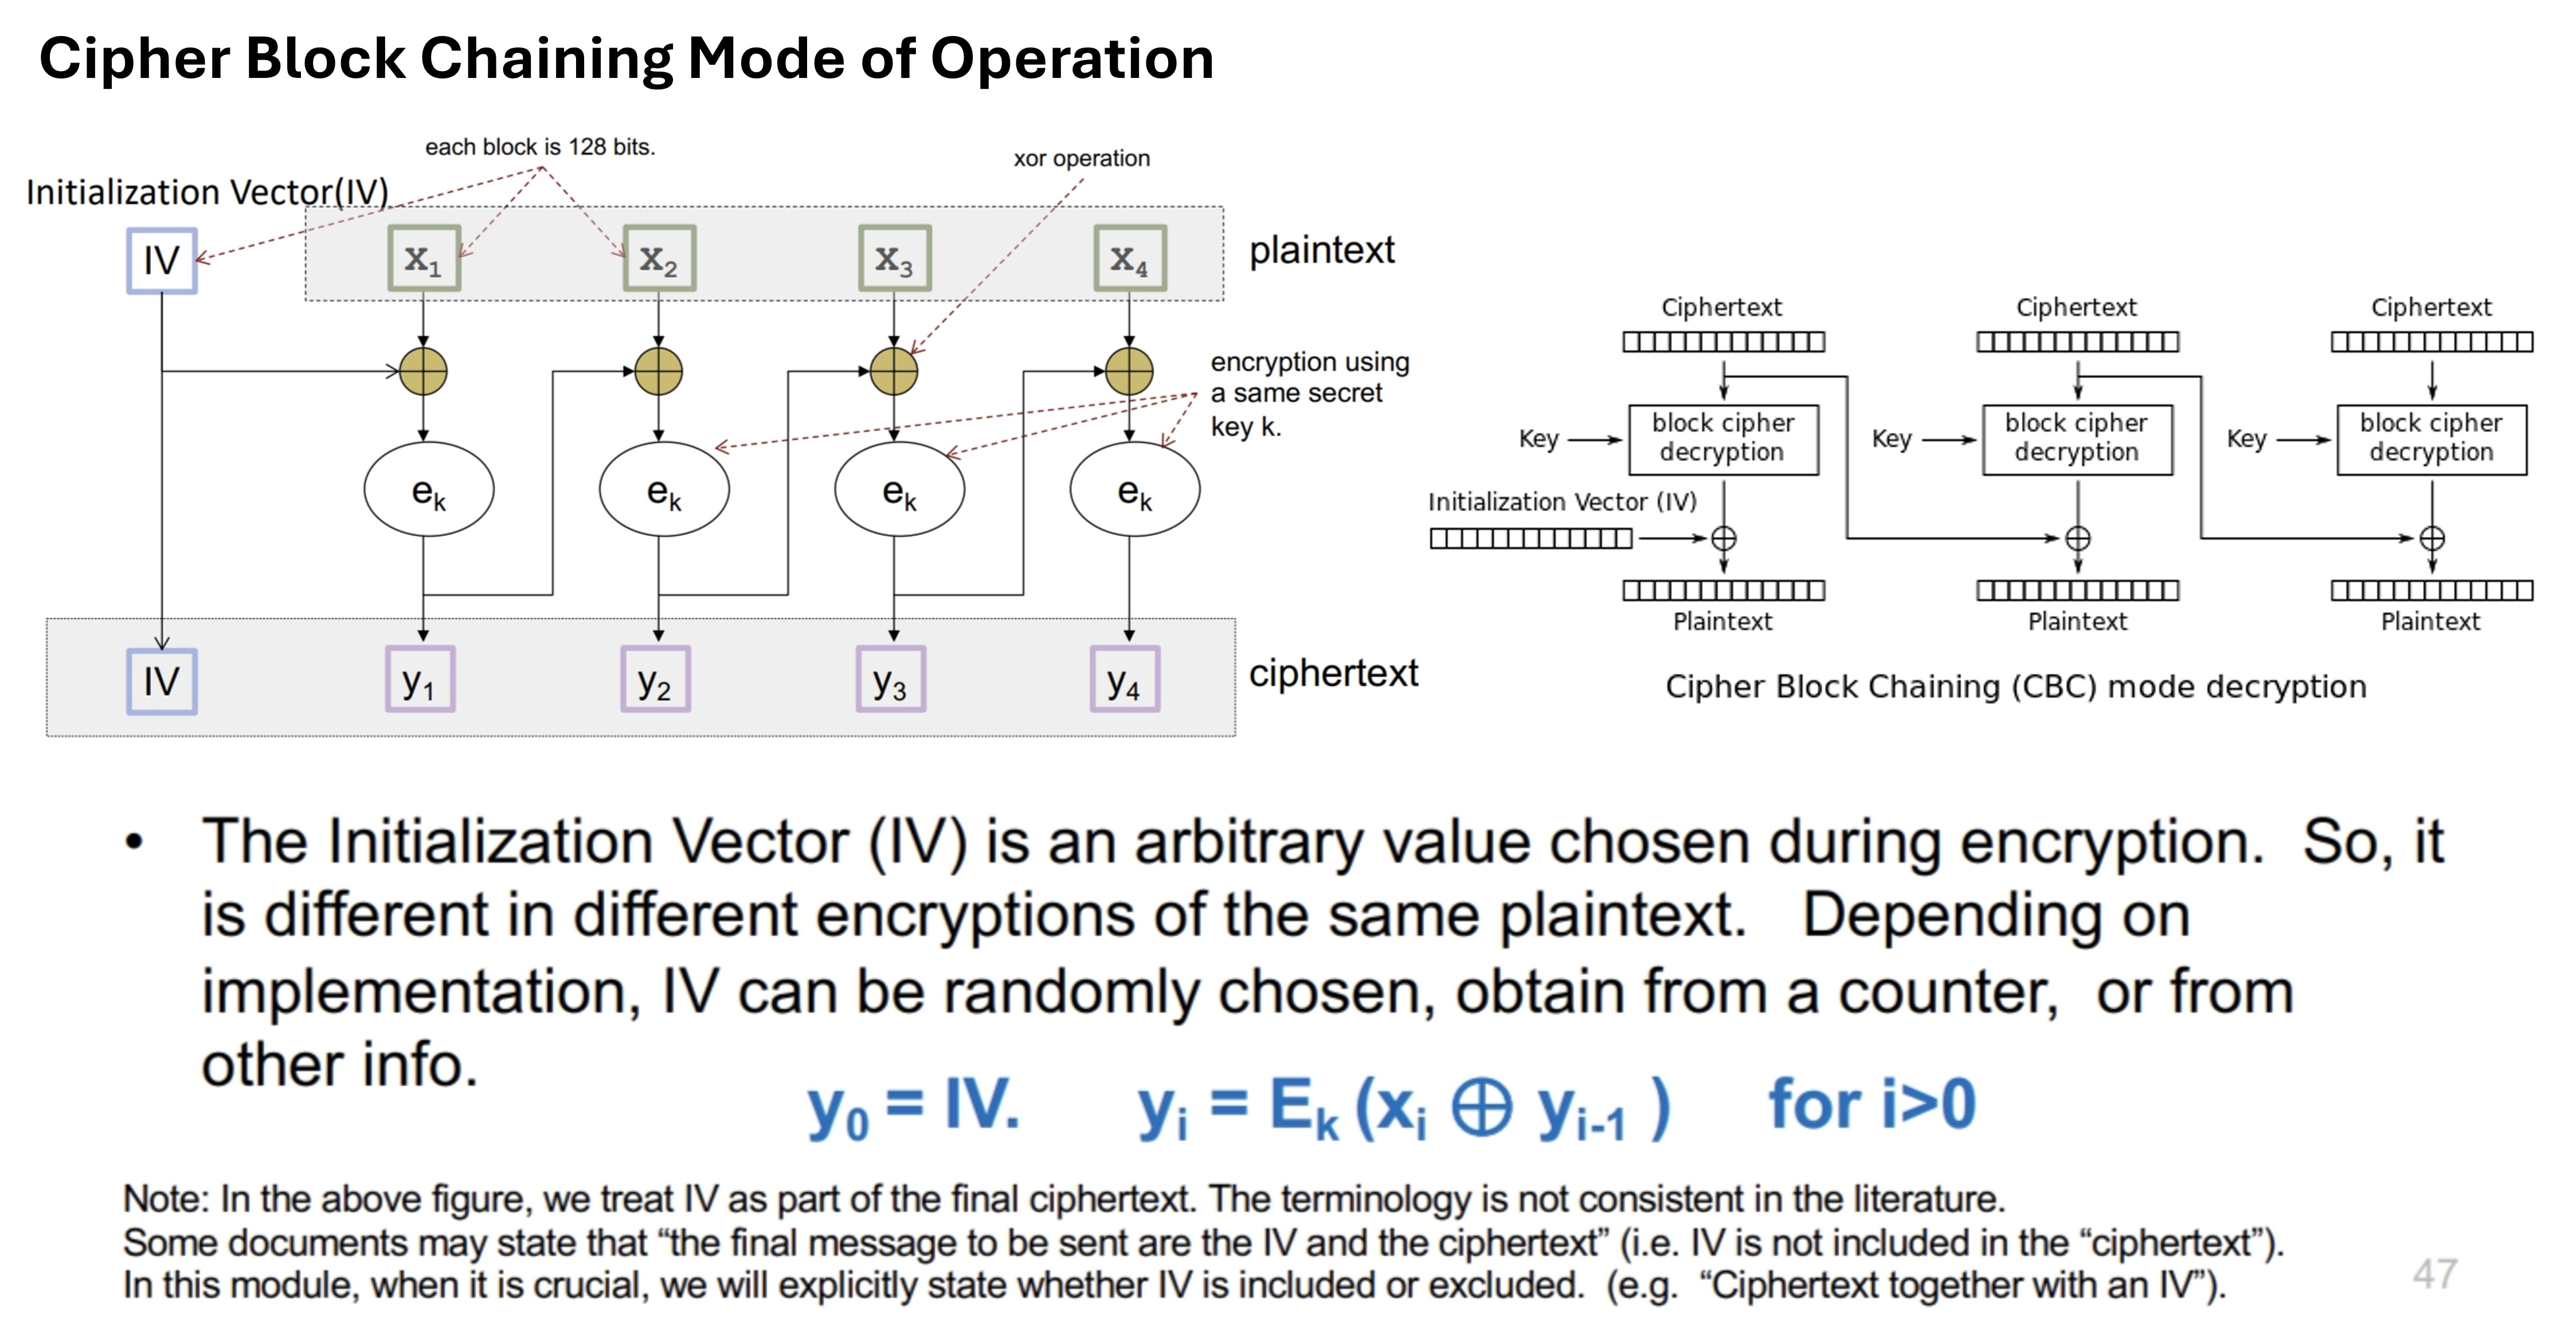
\includegraphics[width=1\linewidth]{CBC}}

\columnbreak
\subsubsection{Mode-of-Operation: Counter Mode (CTR) on AES}
\begin{itemize}
\item \textbf{Counter Mode}: Turns block cipher into stream cipher, generates next keystream block by encrypting successive values of a ``counter''. Counter can be any function producing sequence, incld. simple increment by one counter.
\end{itemize}
\centerline{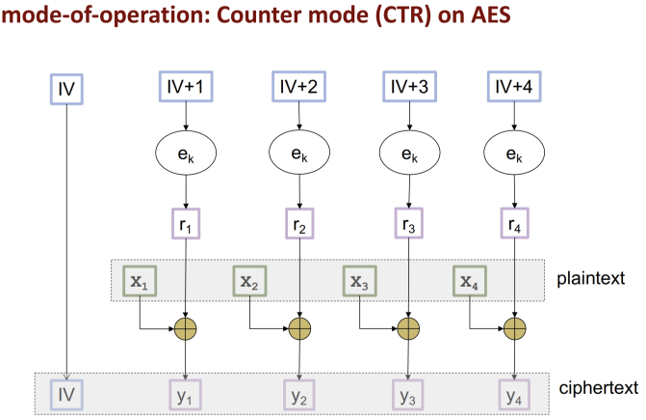
\includegraphics[width=0.5\linewidth]{CTR}}

\subsubsection{Mode-of-Operation: GCM Mode (Galois/Counter)}
\begin{itemize}
\item \textbf{GCM}: Combines Counter mode (CTR) with Galois authentication. Construction of mode more complicated, is ``Authenticated-Encryption''.
\item Ciphertext consists of extra tag for authentication, secure in presence of decryption oracle.
\end{itemize}

\subsubsection{Python Programming: CBC}
\centerline{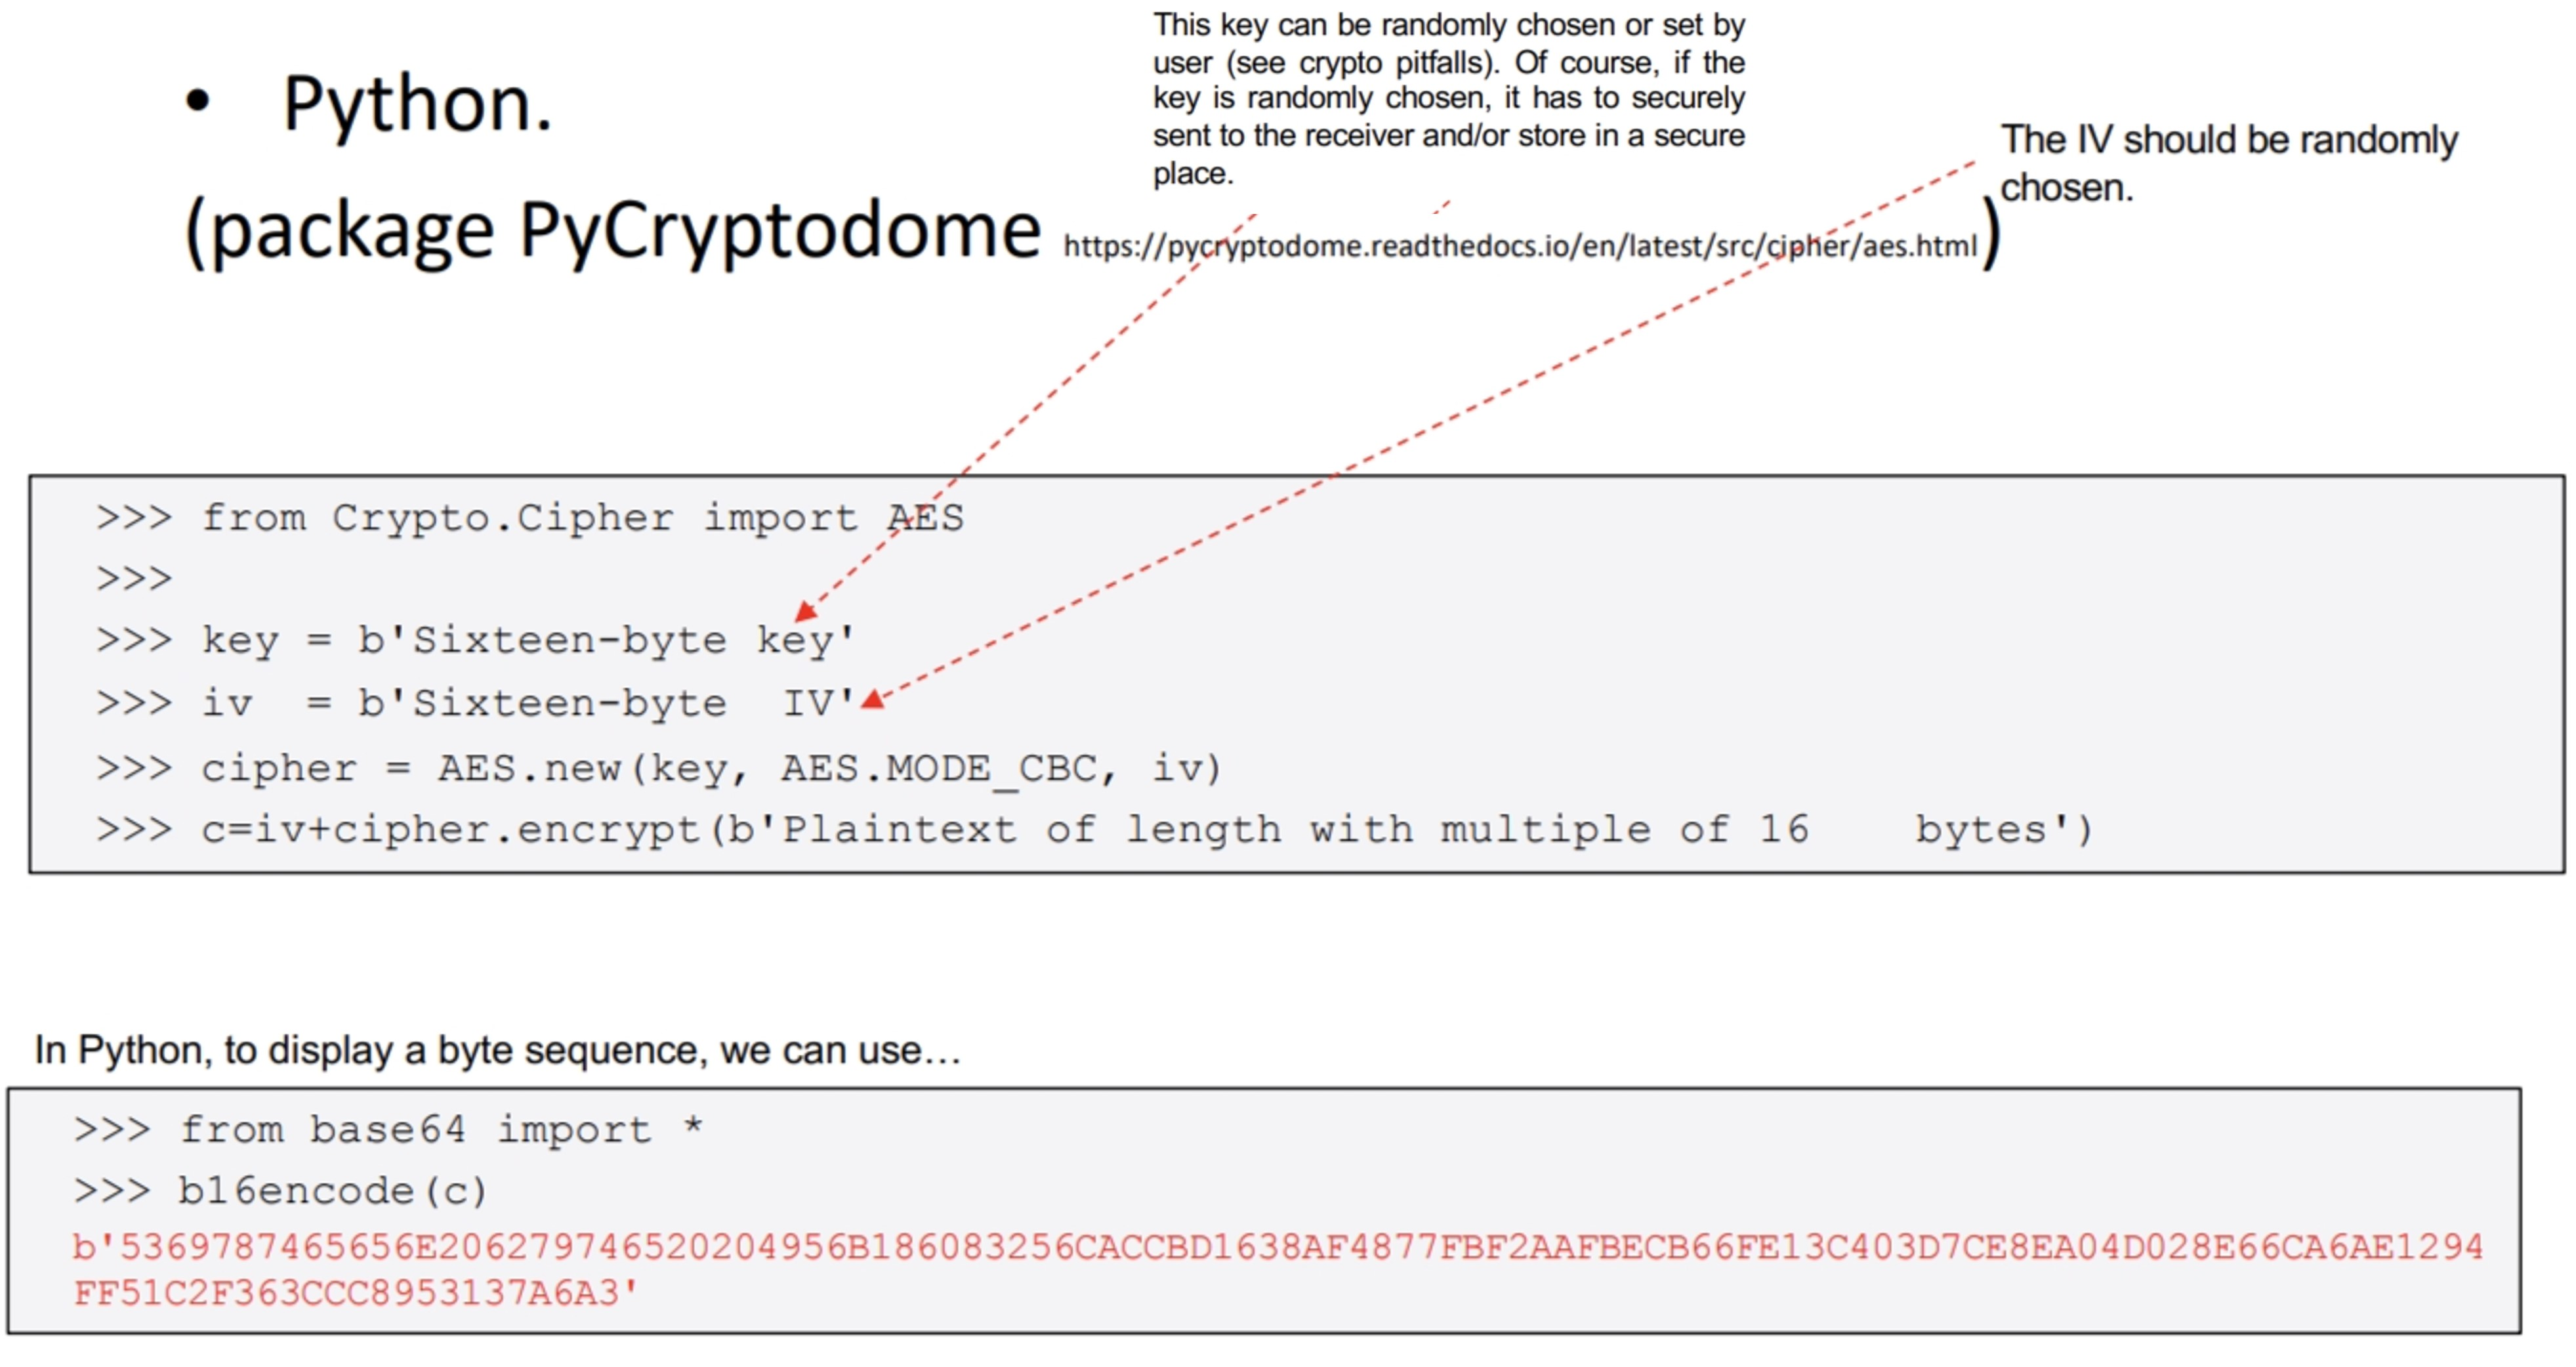
\includegraphics[width=0.95\linewidth]{CBCProgramming}}

\subsection{1.2.3 Stream Cipher and IVs}
\subsubsection{Stream Cipher}
\begin{itemize}
\item \textbf{Stream Cipher}: A symmetric key cipher where plaintext combined with \textbf{pseudorandom cipher digit stream (keystream)}.
\item ``Inspired'' by one-time-pad, generate some cryptographically secure pseudorandom sequence. 
\item w/o knowing secret key, computationally diff. to distingush from truly random sequence. Similarly diff. to get short secret key from sequence, or predict part of sequence from another part.
\item \textbf{IV}: Most ciphers have \textbf{Initialization Vector}, randomly chosen or from counter.
\end{itemize}
\centerline{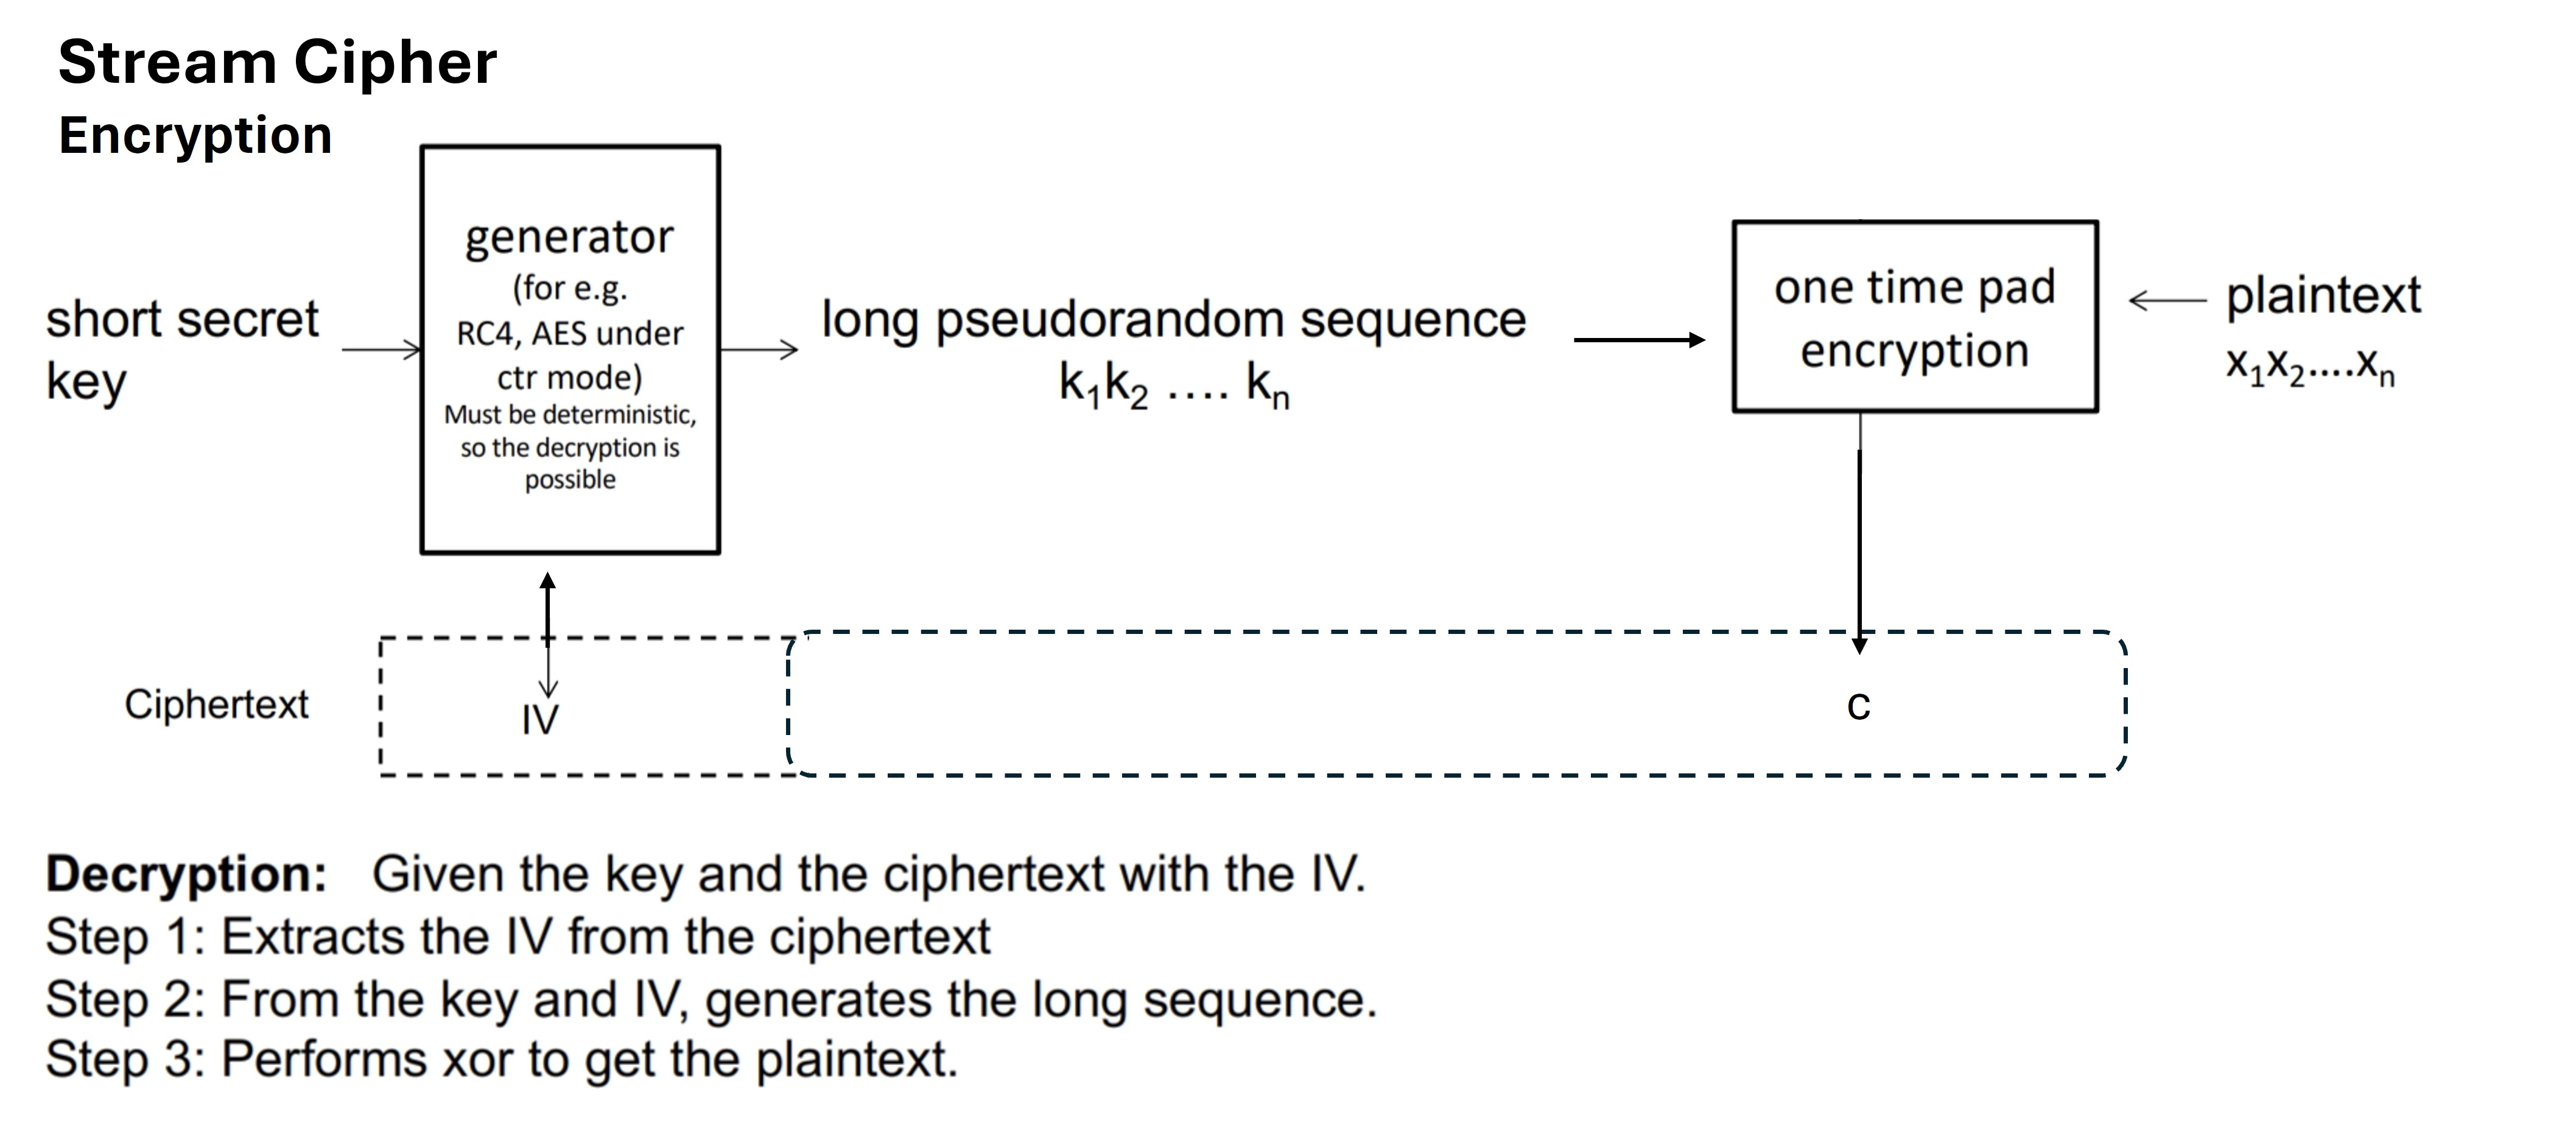
\includegraphics[width=0.95\linewidth]{streamCipher}}

\subsection{Role of Unique IV}
\begin{itemize}
\item Recall, IV appended to front of $c$ to form ciphertext. This IV must be different for every message. IV need not be secret.
\item Sequence is derived from IV and secret key. IV needs to be unique for every message! Otherwise, leaks information.
\item \textbf{Unique IV}: If IV different, two pseudorandom sequences will be different. Two ciphertexts of same plaintext will be different. Can just randomly choose the IV for each message.
\item Hence, xor'ing two ciphertexts will not cancel out pseudomsequences.
\item \textbf{IV makes encryption ``probabilistic.}
\end{itemize}
\centerline{\includegraphics[width=0.95\linewidth]{uniqueIV}}
\begin{itemize}
\item IV also needed in \textbf{CBC mode}, to make encryption non-deterministic. If encryption deterministic (without IV), it will leak information on whether plaintext of two ciphertext are the same, if $C_1 == C_2$. Could be crucial piece of information.
\end{itemize}


\section{1.3 Types of Attacks}

\subsection{1.3.1 Meet-In-The-Middle Attack (Double / Triple DES)}
\subsubsection{Double / Triple DES}
\begin{itemize}
\item \textbf{Double / Triple DES}: To improve DES security, (DES weak as key length of 56 bits short), do multiple repeated encryption using different keys. A reason for this may be to utilize already existing suitable hardware to encrypt.
\item DES does not form a group ( $E_{k1} ( E_{k2} (x) ) \neq E_{k2} (x) $) for some $k3$, so makes sense to use multiple encryption.
\item \textbf{Double DES}: Consider double encryption, we expect key-strength to be 112. ($2^{56 + 56}$). However, attacker, with storage space, can reduce key strength to below 57.
\end{itemize}

\subsubsection{Meet-In-The-Middle Attack}
\begin{itemize}
\item \textbf{MITM}: Meet-in-the-middle Attack, a well-known plaintext attack, is a generic space-time tradeoff cryptographic attack against encryption schemes that perform multiple encryption operations in sequence.
\item Breaking two-part encryption from both sides simultaneously.
\item Primary reason why \textbf{Double DES not used}, and why \textbf{Triple DES key} (168-bit) can be brute forced by attacker with $2^{56}$ space and $2^{122}$ operations.
\item \textbf{Mechanism}: Assume attack has a \textbf{pair ($m, c$)} of plaintext and corresponding ciphertext.
\item \textbf{Remedy}: Use triple encryption, but with 2 keys. (E.g. 3DES, TDES, 3TDES etc.)
\end{itemize}
\centerline{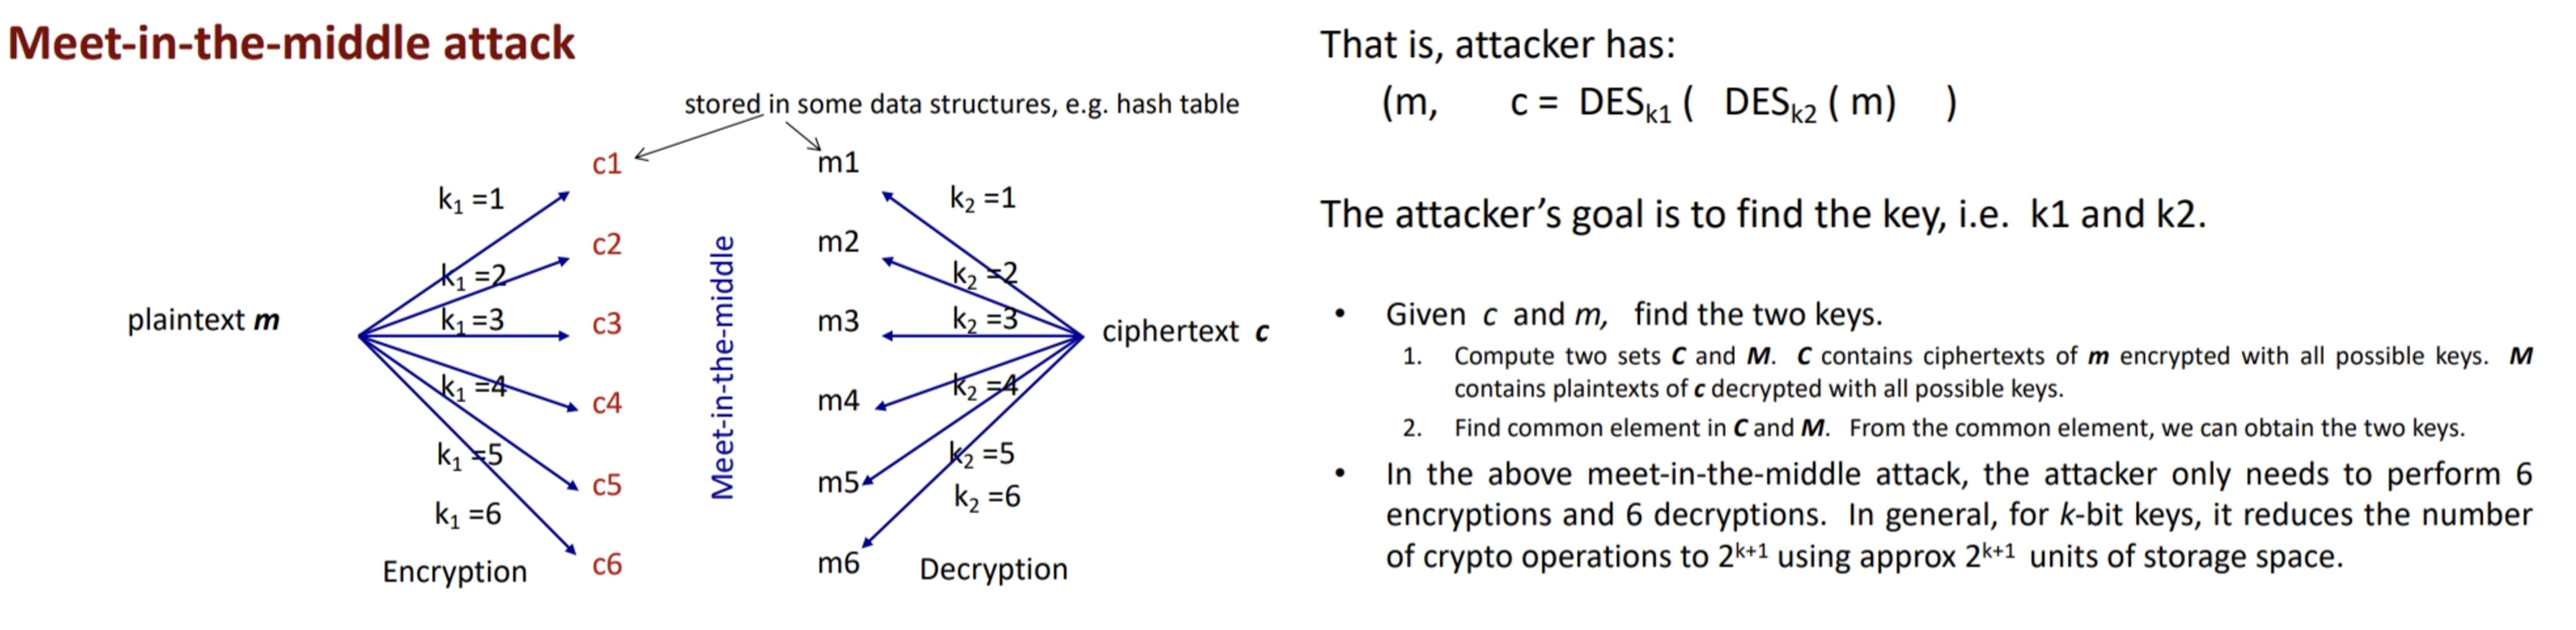
\includegraphics[width=1\linewidth]{MITM}}


\subsection{1.3.2 Padding Oracle Attack}
\subsubsection{Padding Format}
\begin{itemize}
\item For fixed size blocks, e.g. block size of AES is 128bits (16 bytes), padding is needed to fit plaintext into last block.
\item Many ways to fill value, but important piece of information encoded: \textbf{number of padded bits}. If information missing, receiver will not know lenght of plaintext.
\item E.g. \textbf{PKCS\#7 Padding Standard.}
\end{itemize}
\centerline{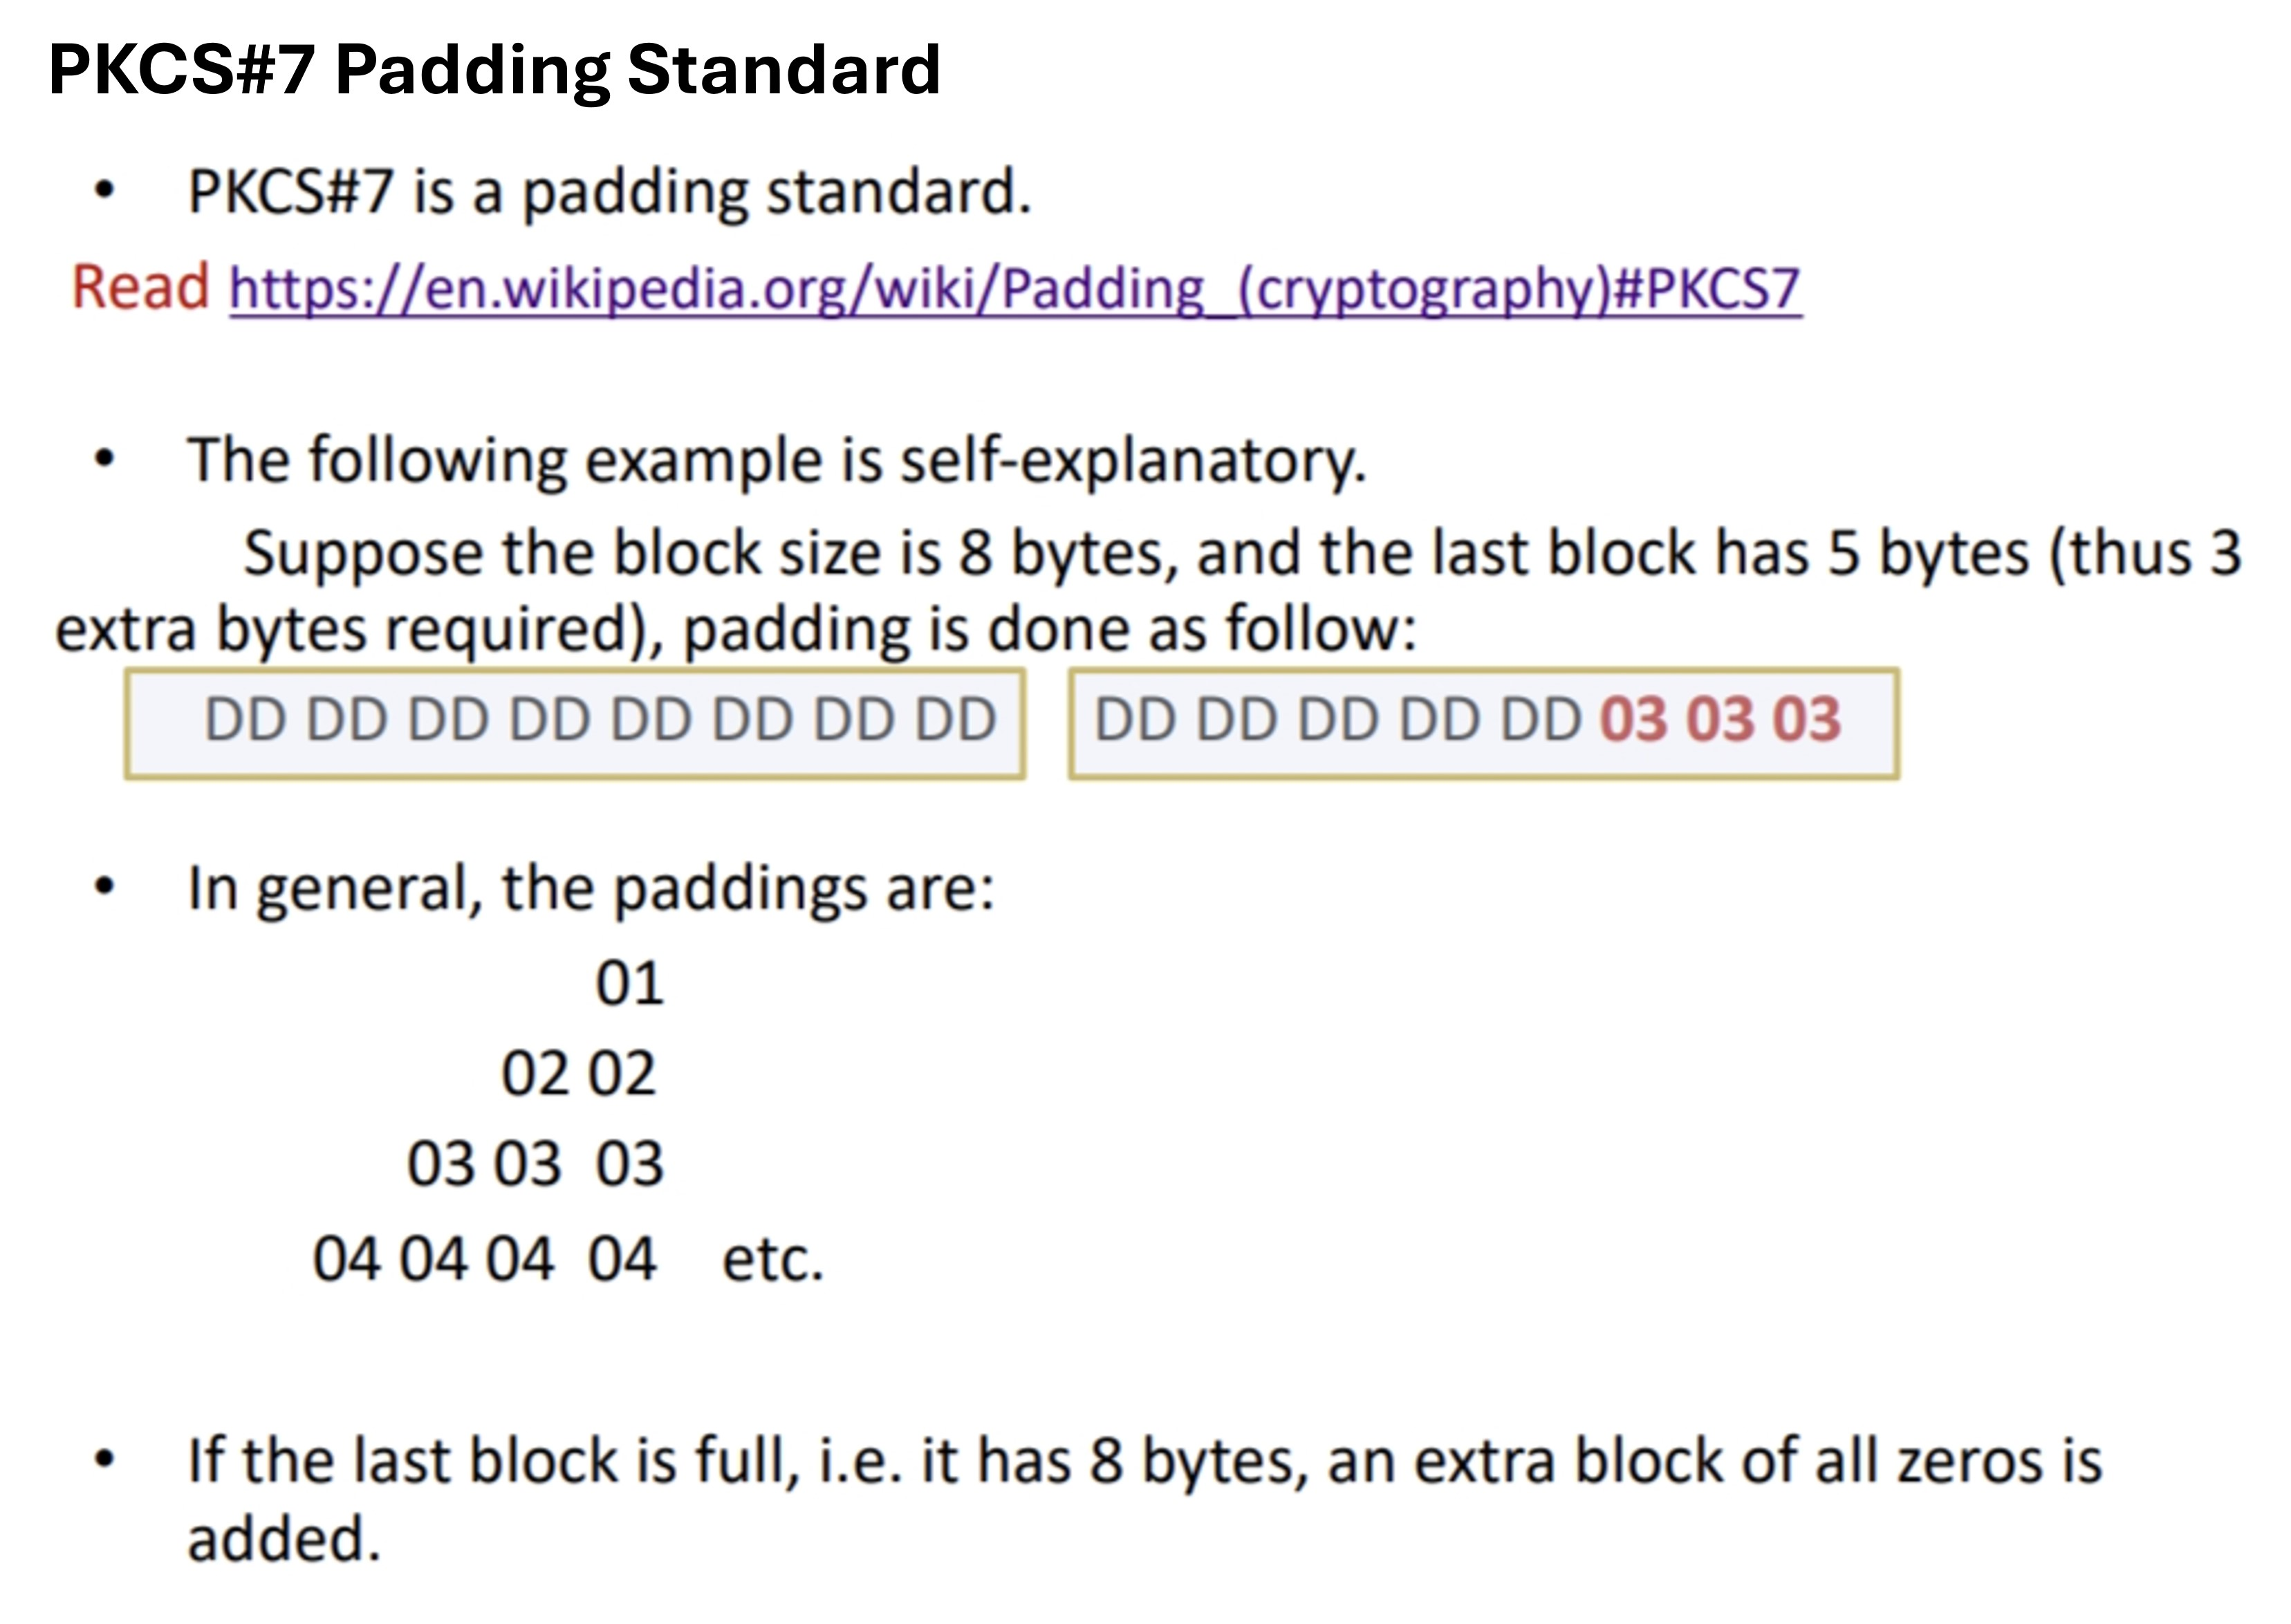
\includegraphics[width=0.8\linewidth]{PKCS7}}

\subsubsection{Oracle}
\begin{itemize}
\item \textbf{Security Analysis}: Need to know \textbf{1. information attackers have}, 2. attacker's goals.
\item \textbf{Oracle}: Query-answer system. Attacker can send in multiple queries, \textbf{Oracle} will output the answer. E.g. \\
-  \textbf{Encryption Oracle}: Output ciphertext for given plaintext, of s. key $k$. \\
-  \textbf{Decryption Oracle:} Output plaintext given ciphertext, of s. key $k$.
\item \textbf{Padding Oracle}: Attacker can query a ciphertext (encrypted using some secret key $k$, padding oracle knows $k$). Oracle outputs yes/no if plaintext is in correct ``padding'' format.
\item Padding Oracle can come in many forms, e.g. query response behavior, response time, subtle differences.
\item \textbf{Padding Oracle Attack Model}: \\
- Attacker has ciphertext including iv: (iv, $c$) \\
- Attack's goal: plaintext of (iv, $c$).
\end{itemize}

\subsubsection{Padding Oracle Attack (on AES CBC Mode)}
\begin{itemize}
\item AES CBC mode not secure against padding oracle attack. (In particular, when done with PKCS\#7).
\item Easily extend algorithm to find all plaintext. Attack is practical as there are protocols between client and server which performs this. \textit{Now, if attack obtained ciphertext, attack can interact with server to get plaintext.}
\item \textbf{Prevention of Padding Oracle Attack}:
	\begin{itemize}
	\item Deny access to such Oracle. Might not be feasible all the time.
	\item Change padding standard to mitigate attack. However, may be smarter way to attack new padding.
	\item Using CTR mode might avoid padding. In practice, bit strings have to be padded in one way or another.
	\item Padding Oracle weaker form of Decryption oracle. If scheme secure in presence of decryption oracle, scheme also secure against padding oracle attack. GCM believed to be IND-CCA2 secure.
	\end{itemize}
\end{itemize}

\columnbreak
\subsubsection{Padding Oracle Attack Algorithm}
\begin{itemize}
\item \textbf{Algorithm}: \\
- Force last X bytes to be padding \\
- Do this by modifying byte of previous ciphertext/IV (Loop till YES) \\
- Here, by XOR'ing padding and input, we get intermediate byte. \\
- By XOR'ing this int. byte with original IV / ciphertext, find plaintext!
\item \textbf{Easily extend algorithm} to find all plaintext, by using increasing length of padding, decrypt from end to start. (Right to Left, repeat process).
\end{itemize}
\centerline{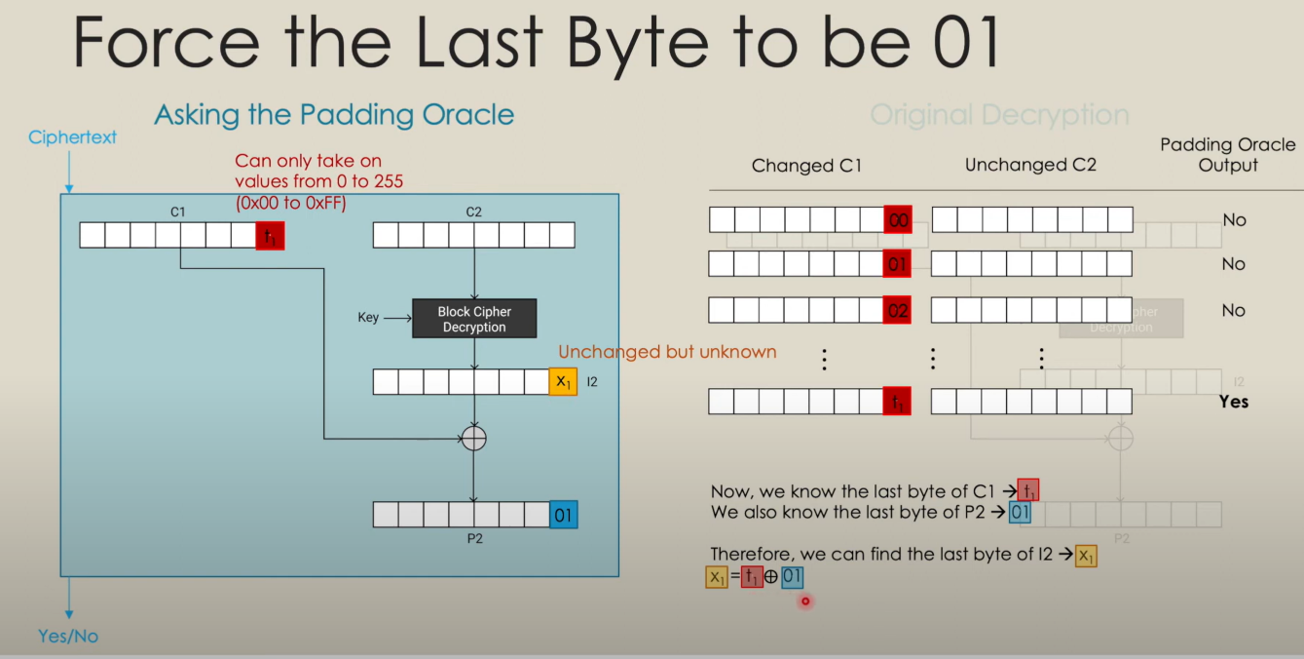
\includegraphics[width=0.8\linewidth]{paddingOracle1}}
\centerline{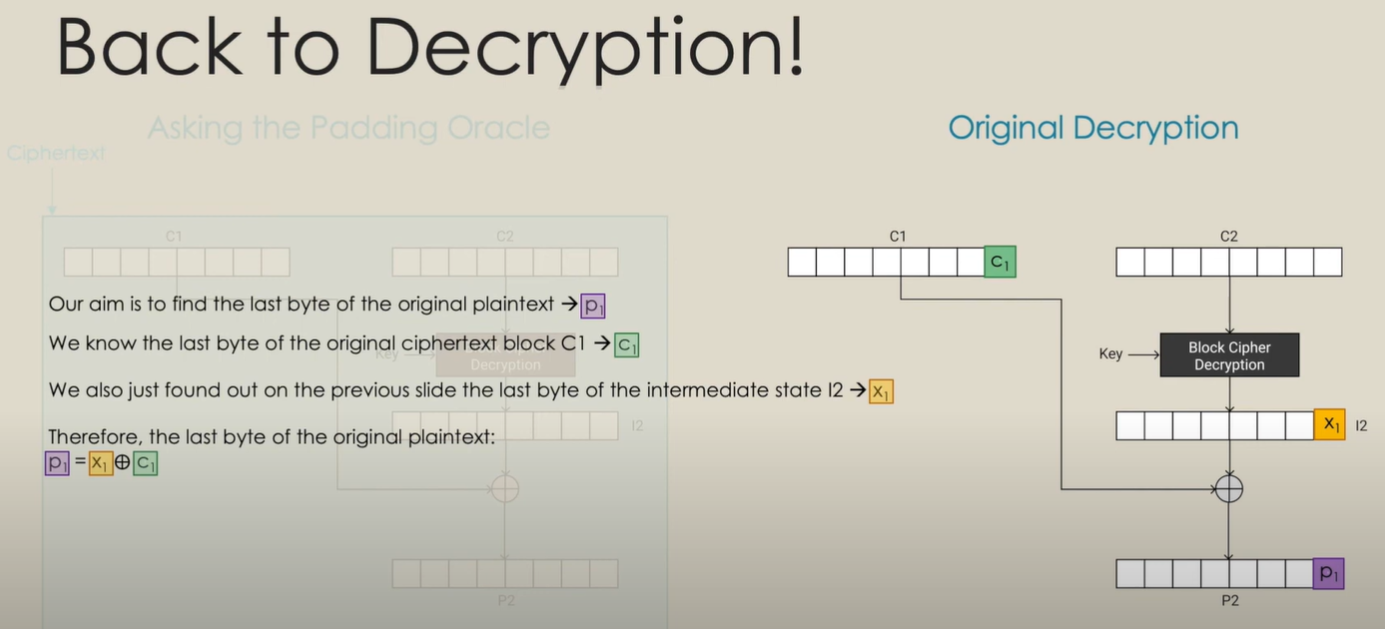
\includegraphics[width=0.8\linewidth]{paddingOracle2}}

\section{1.4 Cryptography Pitfalls}
\begin{itemize}
\item Any secure encryption scheme can be vulnerable if not implemented or adopted properly. Examples include: \\
\textbf{- Predictable Randomness}: Secret key generated predictable, compromise security \\
\textbf{- Modify/Design own encryption scheme}: ``Don't roll your own crypto /security protocol''. Use standard library.
\end{itemize}

\subsubsection{Wrong choice of IV}
\begin{itemize}
\item \textbf{IV Generation}: IV's must not be same for two different ciphertext. 
\item E.g. To encrypt file F, IV derived from filename/meta-data. 
\item E.g. \textit{Microsoft RC4 [implementation] Flaw}, in both Word and Excel, where same IV used when document modified, causing part of documents recovered with negligible amount of computation.
\item When using AES under CBC mode, IV should be unpredictable to prevent certain attack. (E.g. IV = 1, 2, 3). BEAST attack exploits this.
\item \textbf{Reusing one-time pad}: E.g. US Verona Project against Soviets.
\end{itemize} 

\subsubsection{Reliance on Obscurity: Kerchoff's Principle}
\begin{itemize}
\item \textbf{Principle}: System should be secure even if everything about system, except secret key, 
is public knowledge.
\item \textbf{Security through Obscurity}: To hide design of system to achieve security. Not advisable to reveal certain settings (network structure, settings, algorithm, implementation, usernames etc). Obscurity as additional layer in defense-in-depth strategy. Deter, discourage novice attackers.
\item E.g. \textbf{Against relying on Obscurity}: RC4 algorithm was trade secret, but was anonymously posted. MIFARE Classic smartcard also reversed-engineered.
\end{itemize}


\section{2. Authentication Credential}
\begin{itemize}
\item \textbf{Authentication Credential} as any data (PIN, digi. certificate, password) or device that is issued to individual / system used to authenticate identity for purposes of facilitating access.
\item \textbf{Authentication}: Process of assuring communicating entity or origin of piece of information is one it claims to be.
\item \textbf{Authenticity implies integrity}.
\end{itemize}
\centerline{\includegraphics[width=1\linewidth]{communicatingEntity}}
\begin{itemize}
\item \textbf{Authentication Process}: 
	\begin{itemize}
	\item For \textbf{data-origin auth}, one way is to use crypto scheme such as Signature, or MAC (message auth. code).
	\item For \textbf{communication entity auth}, need some authentication protocol employing above crypto primitives.
	\end{itemize}
\item \textbf{Credential}: Unforgeable info required for authentication. (E.g. password is an authentication credential.)
\end{itemize}

\subsection{2.1 Password}
\subsubsection{Password System}
\begin{enumerate}
\item \textbf{Bootstrapping}: User, server establish common password, server keeps file recording identity \textit{(userid, username)} \& \textit{password}. \\
- (Bootstrapping, establish user chosen /or default password.)
\item \textbf{Authentication}: Server authenticates entity. Entity who gives correct password to claimed identity authentic.
\item \textbf{Password Reset}: Many reasons to reset password.
\end{enumerate}

\subsubsection{Weak Authentication System, Replay Attack}
\begin{itemize}
\item Simple sending of identity and password protocol is \textbf{"weak authentication"} system.
\item Such protocol subjected to simple \textbf{"replay attack"}. 
\item Information sniffed from communication channel, replay to impersonate.
\item Under \textit{strong authentication}, info sniffed cannot be used to impersonate.
\end{itemize}

\subsubsection{Attacks on Password System}
\begin{itemize}
\item \textbf{Attack bootstrapping}: Attacks make use of default passwords.
\item \textbf{Attack password reset process}: \textit{Security-Cost Usability tradeoff}: \\
- \textbf{Fallback authentication}: Security Qn / Pw. reset. \\
- Enhance usability, reduce cost but reduce security. \\
- \textbf{Danger}: Social engineering + pw. reset.
\end{itemize}


\begin{itemize}
\item \textbf{Search for correct password}: 
\begin{itemize}
\item \textbf{Exhaustive search}: Test all combinations
\item \textbf{Dictionary Attacks}: Online \& Offline dictionary attacks.
\end{itemize}
\end{itemize}
\centerline{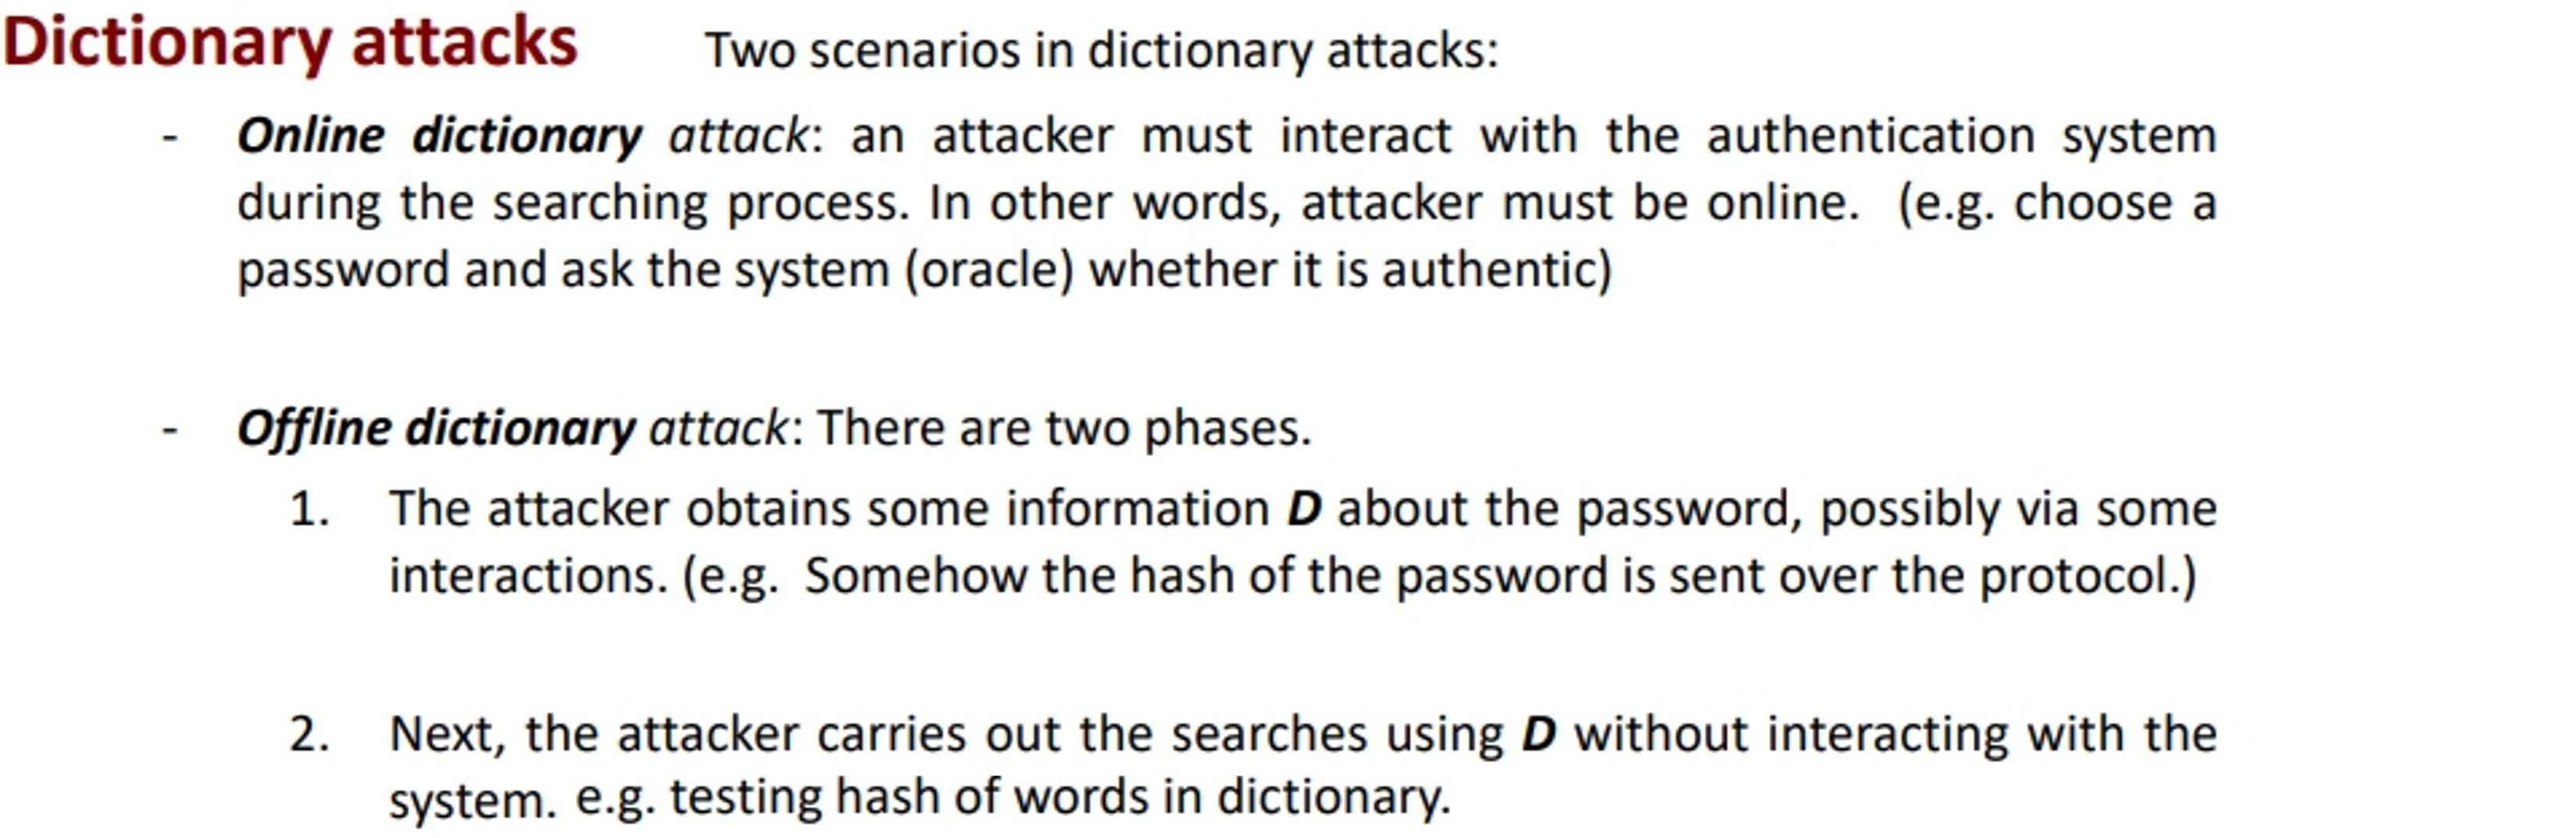
\includegraphics[width=0.95\linewidth]{dictionaryAttack}}

\begin{itemize}
\item \textbf{Stealing of password}: 
\begin{enumerate}
\item \textbf{Sniffing}: Shoulder surfing (look-over-shoulder attack), Sniffing communication (uncommon now, sniffing unencrypted password over public network in clear).
\item \textbf{Viruses, Keylogger}: Computer viruses as key-loggers, or hardware keyloggers. Send captured data back to attack via "covert channel".
\item \textbf{Phishing}: Trick to voluntarily send password to attacker. Social engineering attack. \\
- \textbf{Spear Phishing}: targeted attack against particular small group of users. \\
- \textbf{Phishing, Pharming, Vishing, Smishing} \\
- \textbf{Prevention}: User training, blacklisting.
\item \textbf{Cache}: Shared workstation where information is cached.
\item Lost of password file
\end{enumerate}
\end{itemize}

\subsubsection{Password Strength}
\begin{itemize}
\item \textbf{Password Entropy}: Measure of (randomness) password strength. 
\end{itemize}
\centerline{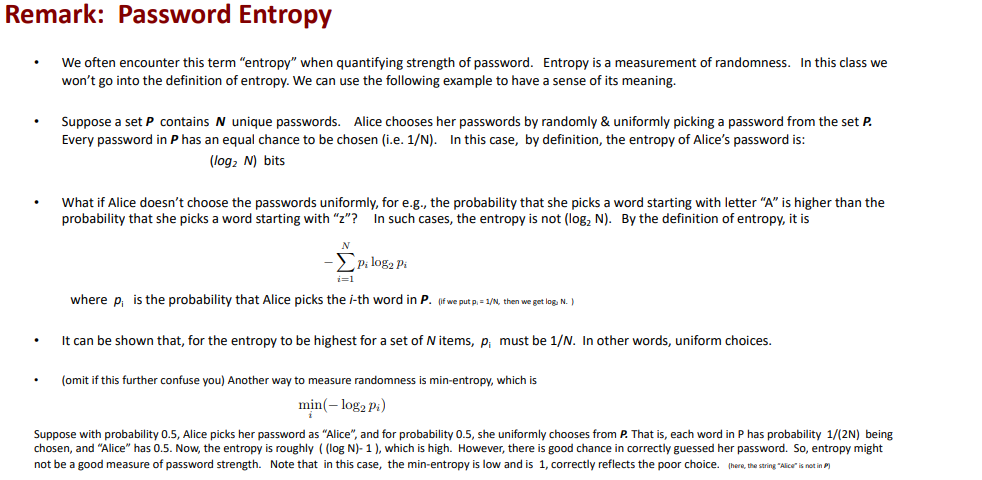
\includegraphics[width=1\linewidth]{passwordEntropy}}
\begin{itemize}
\item Truly random password high "entropy", difficult to remember. User selection biased. Human generated 20-digit password likely to attain 
entropy much less than 20 $log_2(10)$.
\item RFC 4086 suggests password at least 29 bits of entropy to secure against \textbf{online attacks}.
\item If cryptographic keys generated from password, \textbf{offline attacks} possible, password should have at least 128 bits of entropy.
\end{itemize}


\begin{itemize}
\item \textbf{Online vs. Offline attack}: Need to communicate with server not under control to check whether password is correct.
\item E.g. WPA2 personal vulnerable to offline dict. attack. Some "hash" of password sent in clear.
\item \textbf{Enhance password system}: \\
- Make online attack difficult by adding intentional delay / lock. \\
- Make offline attack difficult by applying KDF to password. \\
- System check for weak password / regular changes of password.
\item \textbf{Password vs. Secret Key}: \\
- KDF: key derivation function. \\
- Password as source for crypto secret key. \\
- Using cryptographic hash, hash multiple times to form key, increase cost of exhaustive search. Tradeoff utility.
\end{itemize}

\columnbreak
\begin{itemize}
\item \textbf{Password Files}: \\
\textbf{Hashing}: \\
- File stores userid, password. Add additional layer of protection. \\
- Password file should be "hashed" and "salted"! \\
- (Not "encrypted", don't want way to decrypt and get back) \\
- To authenticate, store and compare hash. \\
\textbf{Salt:} \\
- Need same password hash to two diff. values, for two diff. userid. \\
- (Rainbow table: precomputed table caching outputs of crypto hash function to crack hashes) \\
- Achieve this by salting. New salt randomly generated, concat to pw., output different hash. Salt and hash stored in database.
\end{itemize}

\subsubsection{ATM Skimming}
\begin{itemize}
\item Demonstrates password stealing.
\item Authentication: User presents card, and PIN.
\item Data encoded into magnetic strip using well-known standards, easy to "copy" card by reading and writing to spoofed card.
\item ATM Skimmer: card-reader, camera overlooking keypad / spoofed keypad, some means to record, transmit.
\item \textbf{Measures}: Anti-skimmer devices, shielding keypad, increase awareness, change to unforgeable smartcard.
\end{itemize}

\subsection{2.2 Biometric}
\begin{itemize}
\item \textbf{Biometric data as password}. For identification, or verification.
\item \textbf{Enrollment}: template of user biometric data captured, stored (bootstrapping). \textbf{Verification}: capture biometric data, compare using matching algorithm.
\item Inevitable noise capturing biom. data, leading to error in matching. \\
- \textbf{FMR (False Match Rate)}, \textbf{FNMR (False non-match rate)}. \\
- Adjust threshold to adjust FMR \& FNMR. \\
- \textbf{EER} (Equal Error Rate, FNMR = FMR) \\
- \textbf{FER} (False-to-enroll rate, users' data uncaptureable, e.g. injury)  \\
- \textbf{FTC} (Failure to capture rate, uncaptureable during auth, e.g. finger dirty
\end{itemize}
\centerline{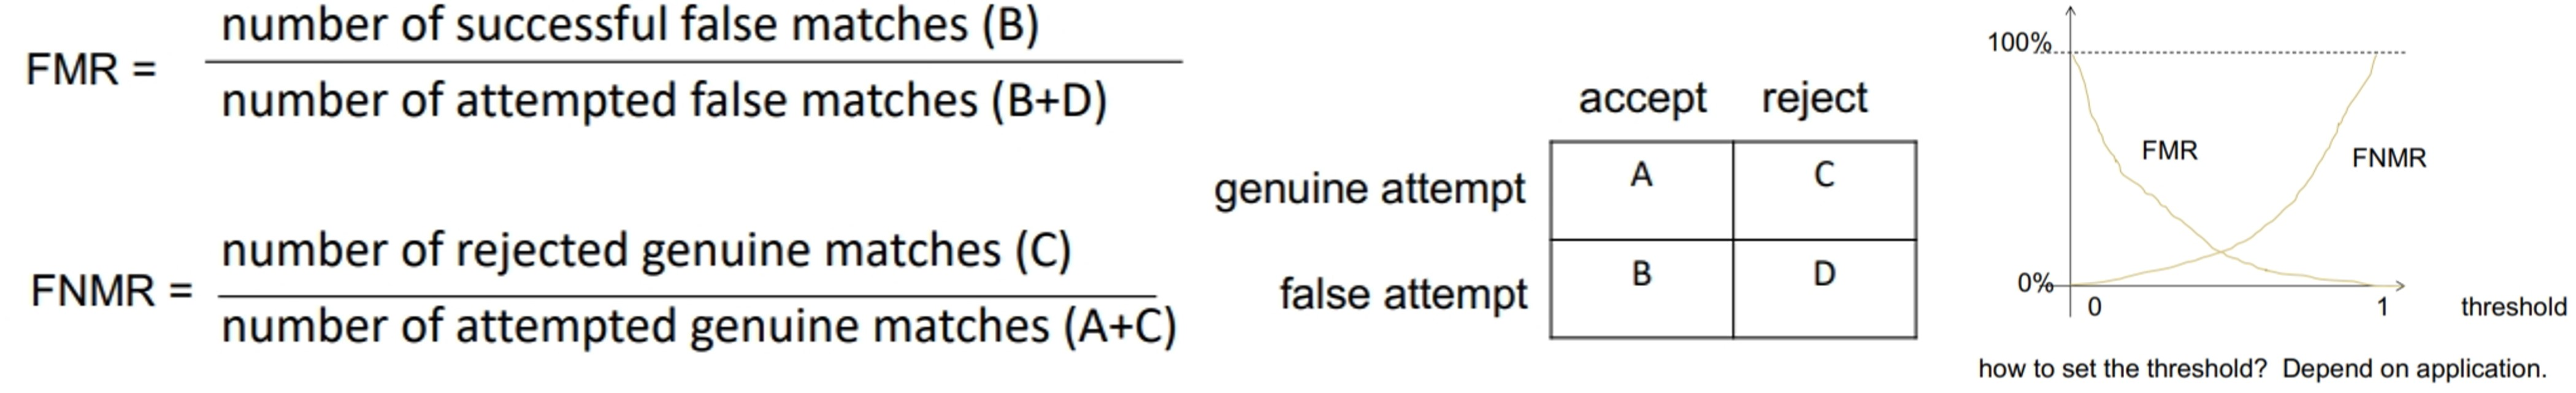
\includegraphics[width=1\linewidth]{FMR}}
\begin{itemize}
\item \textbf{Fingerprint as biometric}: performance depends on quality of scanner, EER range from 0.5\% to 5\%.
\item Biometric data easily spoofable, include \textit{liveness detection} to verify entity.
\end{itemize}

\subsection{2.3 Multi-factor / Multi-step Authentication}
\begin{itemize}
\item \textbf{n-factor Authentication}: Require $n$ authentication factors.
\item \textbf{"Factors"}: \textbf{Know} (Pw, PIN), \textbf{Have} (card, phone, token), \textbf{Are} (Biometric).
\item Must be distinct factors for multi-factor (Know + Have, Have + Are) etc.
\item One Time Password token: \textbf{Time-based /or Sequence-based}.
\item \textbf{2-Step Verification}: Both same factor, e.g (email + password, both "what-you-know", cannot be called "2-factor".)
\item \textbf{out-of-band}: In 2-step verification, two communication channels, main and separate for add. authentication. Non-main called "out-of-band" channel, assume attacker unable to compromise both channels.
\end{itemize}



\columnbreak

\section{3. Authenticity (Data Origin)}

\subsection{3.1 Crypto Primitive: Public Key Cryptography}
Public key crypto primitive includes public key encryption and signature. Goal is for confidentiality, and authenticity.
\begin{itemize}
\item Symmetric-key encryption uses same key for encrypt, decrypt.
\item \textbf{Public Key (Asymmetric-key) scheme}: Uses different keys for encryption and decryption.
\item Decryption algo also needs public key. When said "using private key to decrypt", this means using both.
\end{itemize}
\centerline{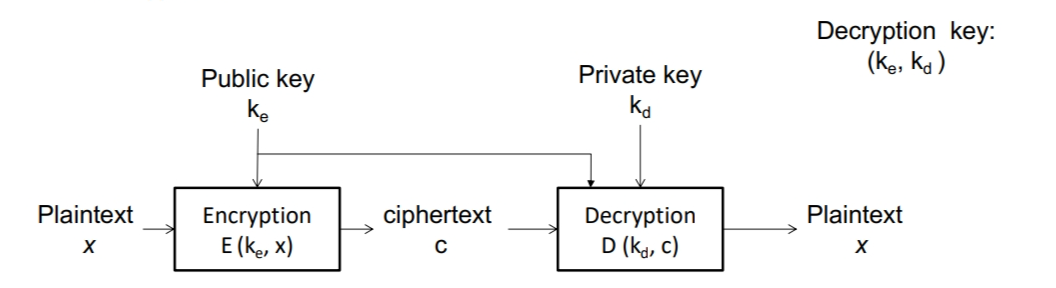
\includegraphics[width=1\linewidth]{publicKeyCrypto}}

\begin{itemize}
\item \textbf{Security Requirement}: Given public key \& ciphertext, difficult to determine private key \& plaintext. (Encryption oracle accessible.)
\item \textbf{(PKC) Public Key Crypto}: Handles scenario of sharing symmetric key via secure channel. PKC only requires secure broadcast channel to distribute the public key. However, building secure broadcast channel to distribute public key is challenging.
\item \textbf{PKC:} Useful for encryption, important application is in authentication (e.g. HTTPS). Limitations compared to symmetric in speed.
\end{itemize}
\centerline{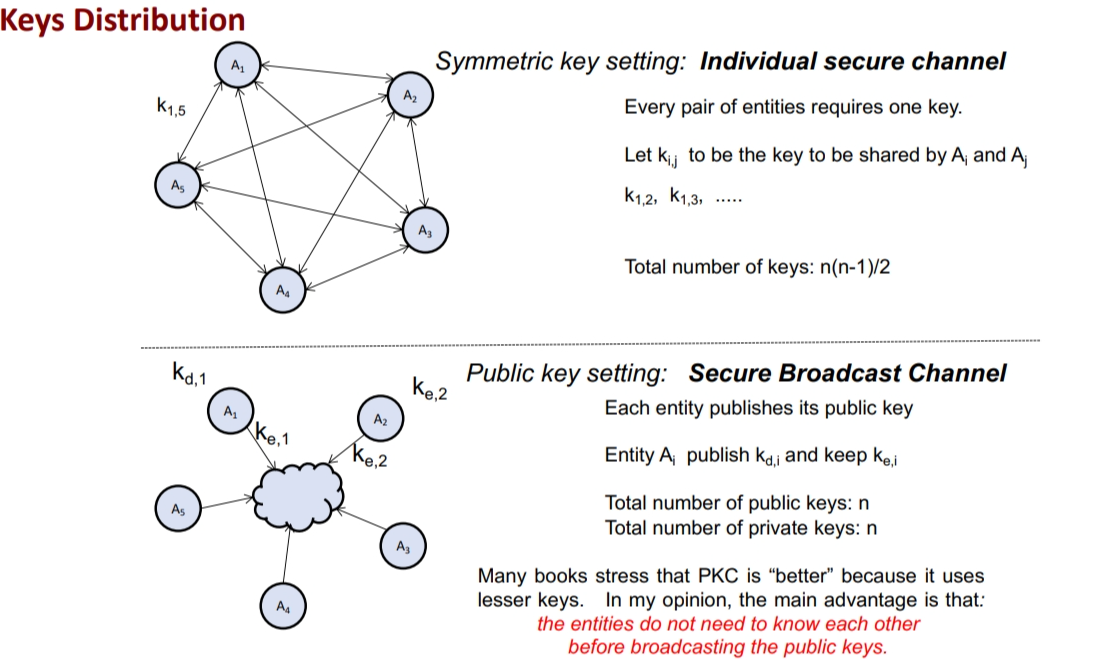
\includegraphics[width=1\linewidth]{keyDistribution}}
\begin{itemize}
\item \textbf{Remark}: Many PKC represent data as integers, algo used are some arithmetic operation on integers, represented using binary.
\item A 1024-bit key is represented under binary representation. An algorithm exhaustively searches 1024-bit integers ($2^{1024}$) is infeasible.
\item For this course, we will consider \textbf{"classroom" RSA}, most basic form RSA.
\item \textbf{In Practice}: Padded RSA (to destroy some property), choose strong primes, fast secure ways to generate primes, secure implementation to guard against side-channel attack, "e" is fixed mostly at 65537. Considerations of quantum computer.
\end{itemize}

\subsubsection{Popular PKC Schemes}
\textbf{RSA}: Key size - 2048 bits. \\
\textbf{ElGamal}: Exploit techniques in Elliptic Curve Cryptography (ECC), reduce key size to - 300 bits. \\
\textbf{Paillier}: Partial homomorphic with respect to addition.



\subsection{Public Key: RSA ("Classroom RSA")}
\centerline{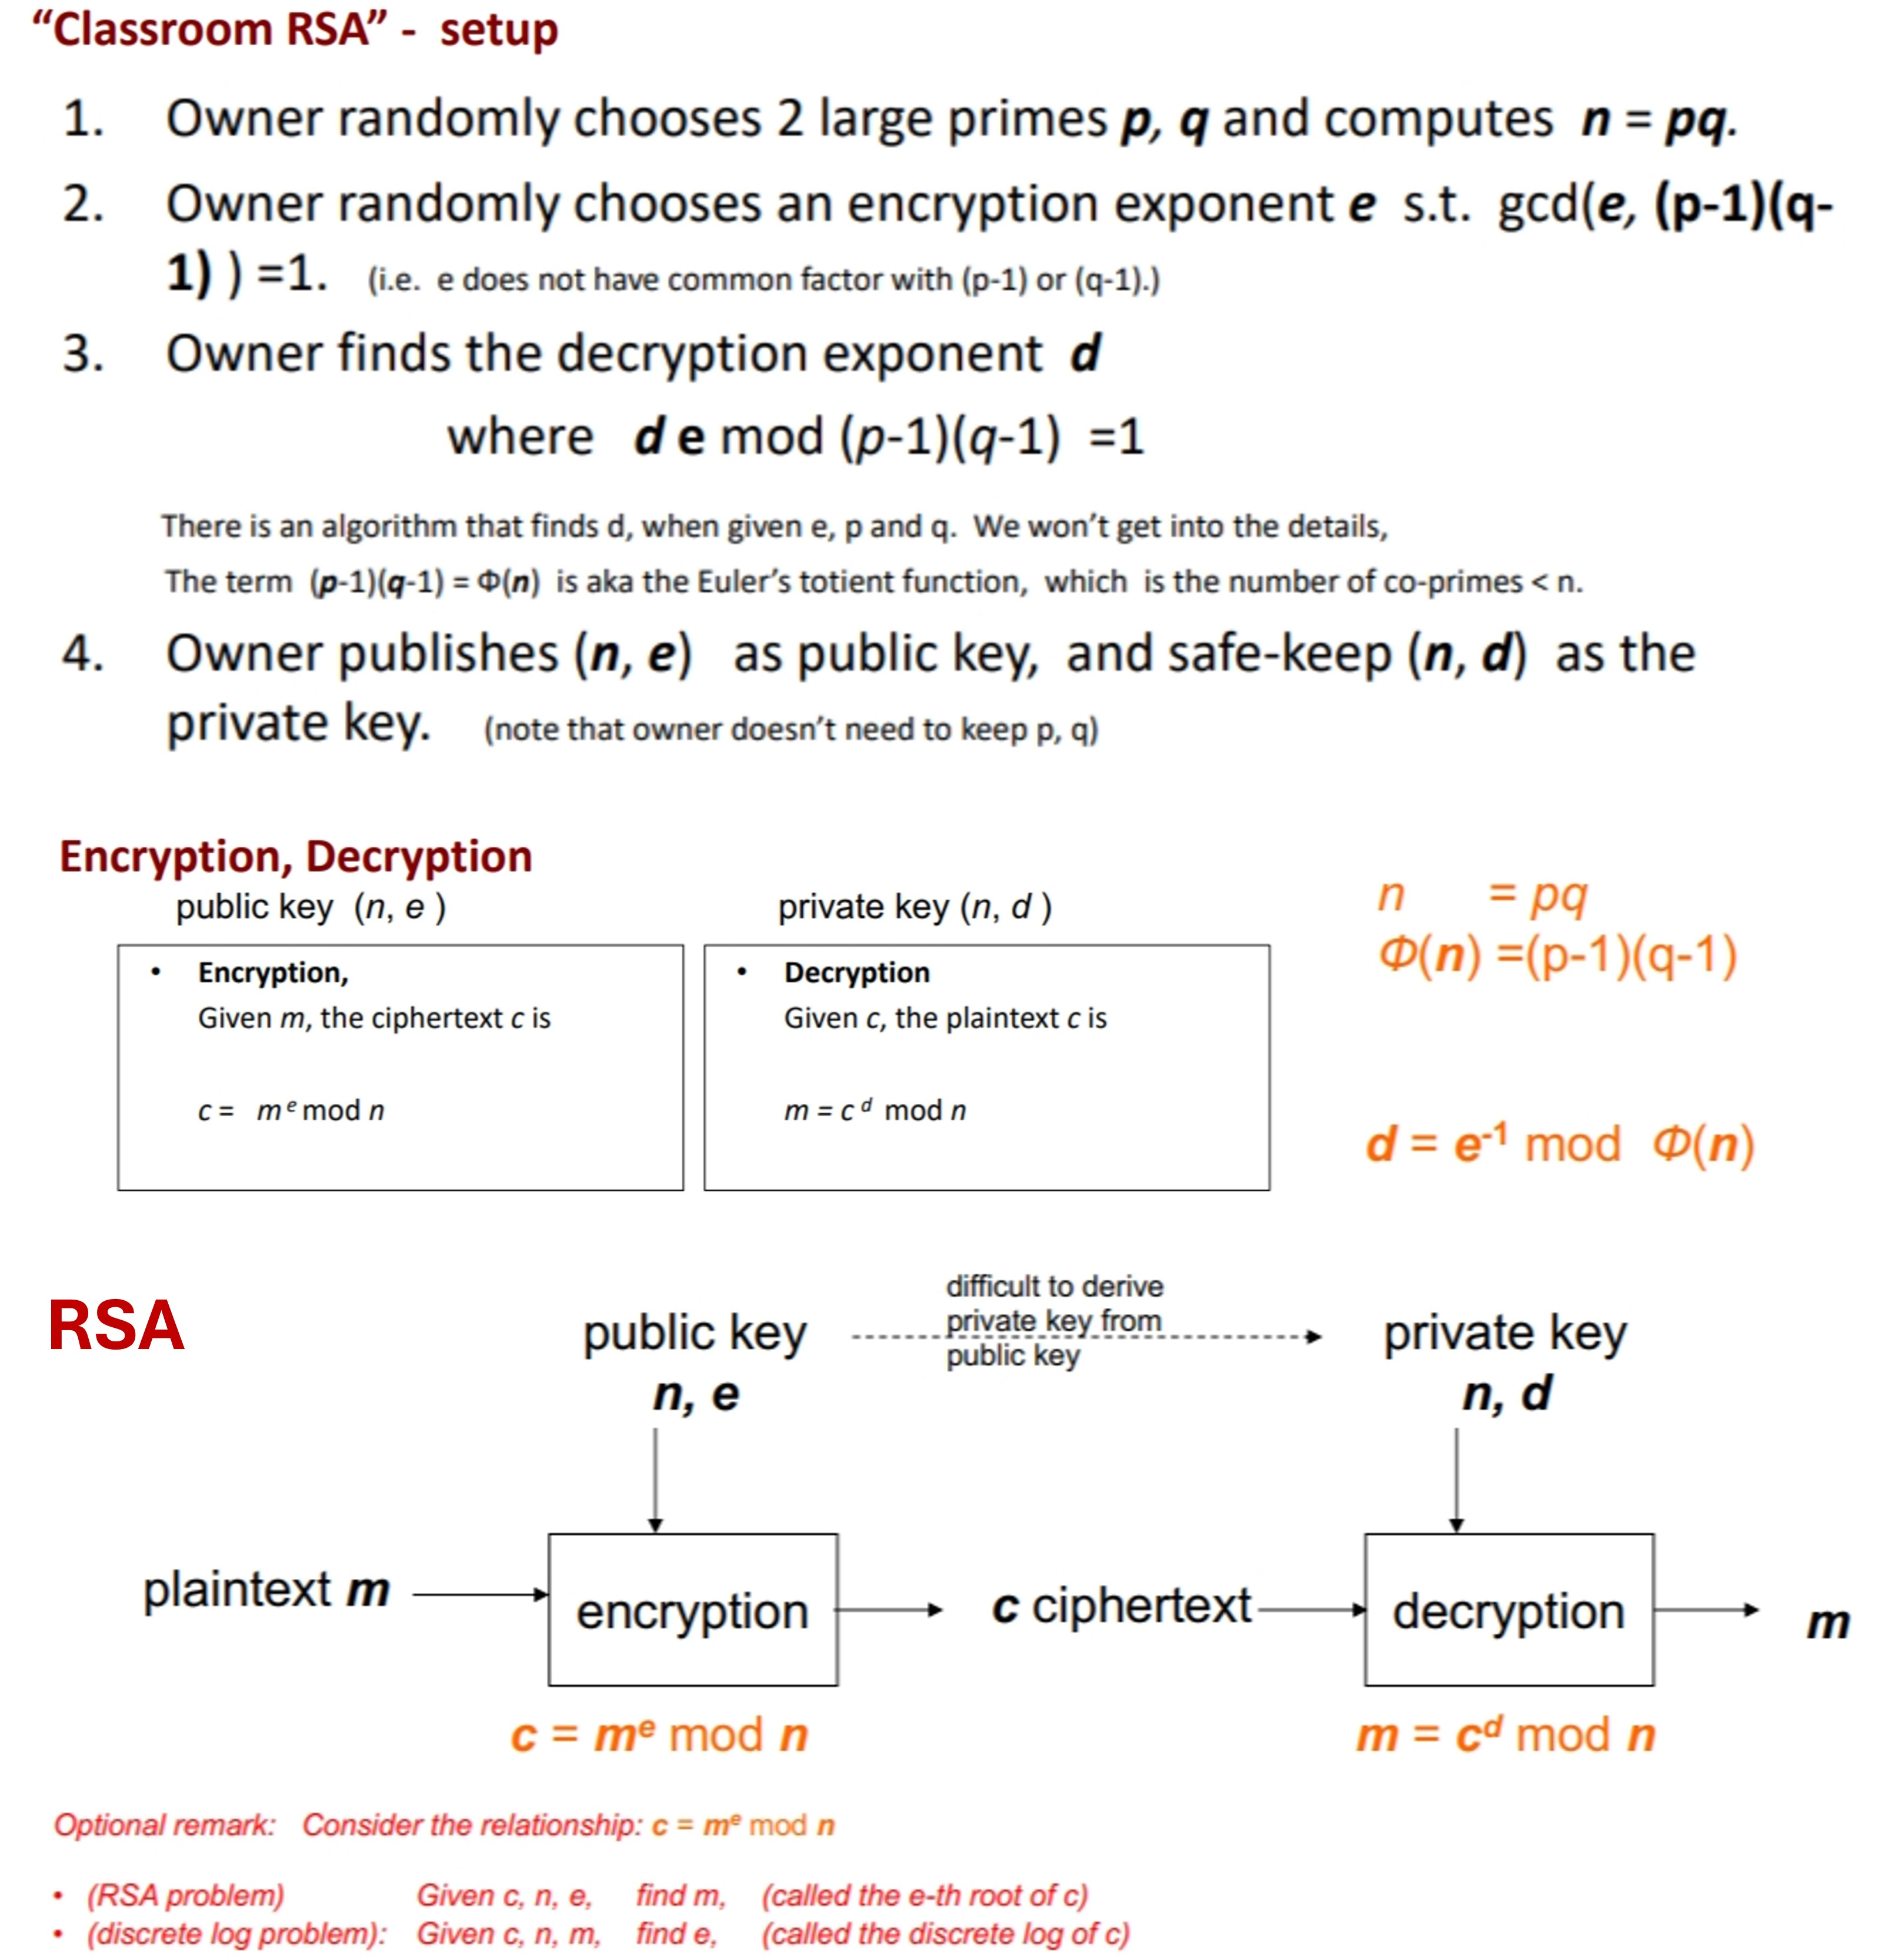
\includegraphics[width=1\linewidth]{classroomRSA}}
\begin{itemize}
\item \textbf{Correctness of RSA}: For any positive $m < n$, and any pair of public/private keys, that \textbf{Decrypt(Encrypt($m$)) = $m$}.
\item $(m^e)^d$ mod $n$ = $m$
\item Correctness depends on the property of modulo.
\end{itemize}
\centerline{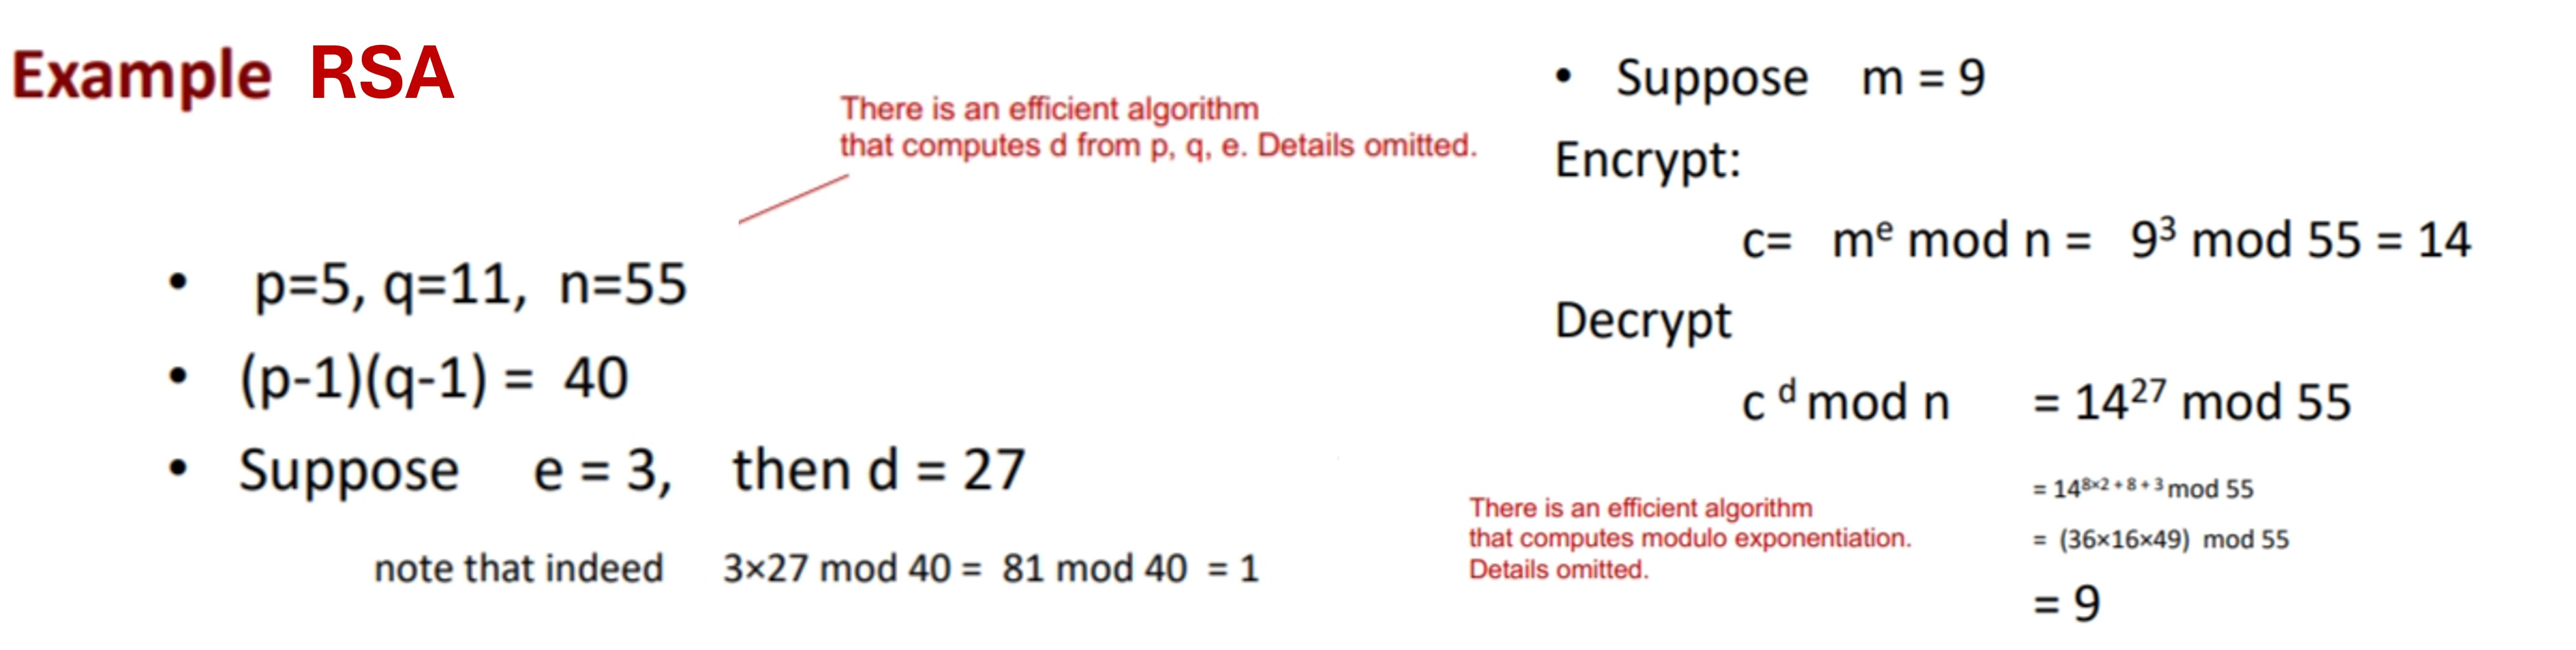
\includegraphics[width=0.9\linewidth]{RSAexample}}
\begin{itemize}
\item \textbf{Interchangeable role of encryption \& decryption key}: Swap role of $d$ and $e$, public can decrypt, owner can encrypt. Usually does not hld in other PKC. This property useful in designing \textbf{signature scheme}.
\item \textbf{Algorithmic Issues}: There is efficient algo to compute exponentiation, hence, efficient way to encrypt, and decrypt (given $n, m, e$, find $m^e$ mod $n$ for encrypt, given $c, d, n$, computer $c^d$ mod $n$).
\item \textit{Step 1 setup}:  Find random prime, randomly pick number, test if prime. (Primality Test). 
\textit{Step 3 setup}: Value of $d$ efficiently computable from $e$ and $n$ using \textit{extended Euclidean algorithm}.
\end{itemize}

\subsubsection{Security of RSA}
\begin{itemize}
\item Getting RSA private key from public key as difficult as factorizing $n$.
\item However, not known whether the problem of getting plaintext from ciphertext as difficult as factorization.
\item \textbf{post-Quantum cryptography}: Generally refers to PKC that are secure against quantum computer.
\item Significant efforts to migrate current systems to post-quantum crypto (Quantum possibility to render RSA algo insecure by 2030). From 2016, NIST plans to choose standard by 2024. Four candidates for Rd 4 (2022). 
\end{itemize}

\subsection{Summary of Data Authenticity}
\null
\centerline{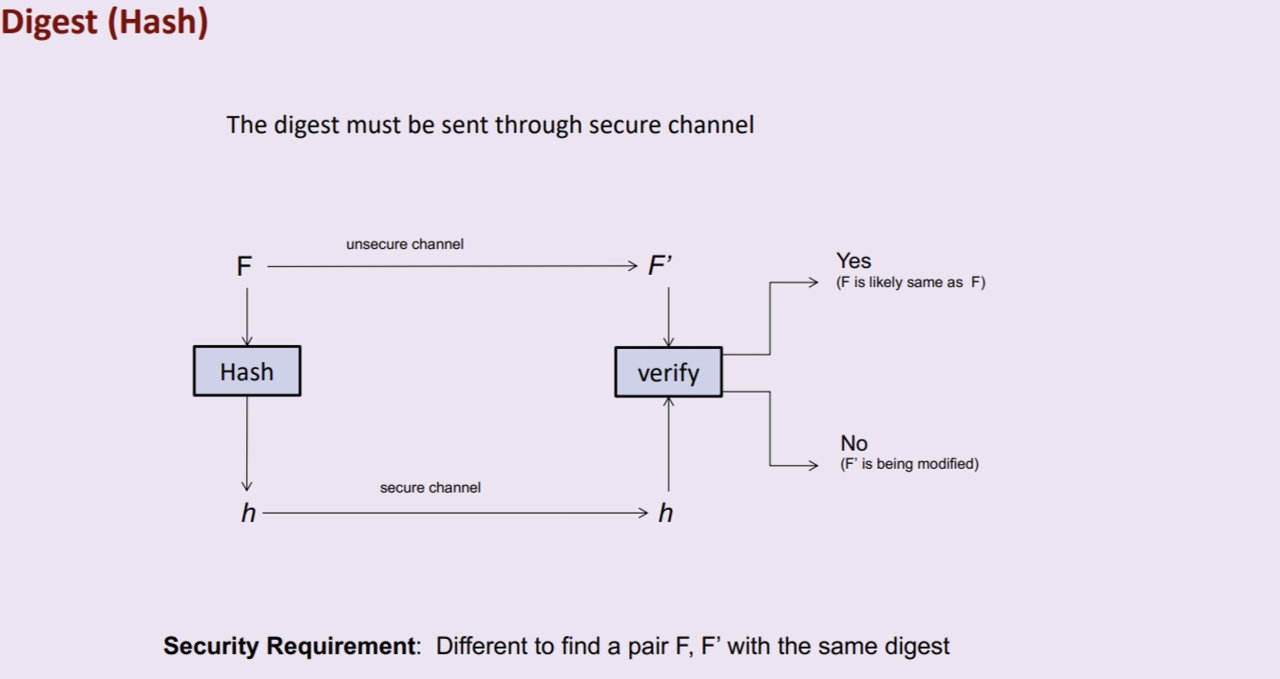
\includegraphics[width=1\linewidth]{authSummary1}}
\null
\centerline{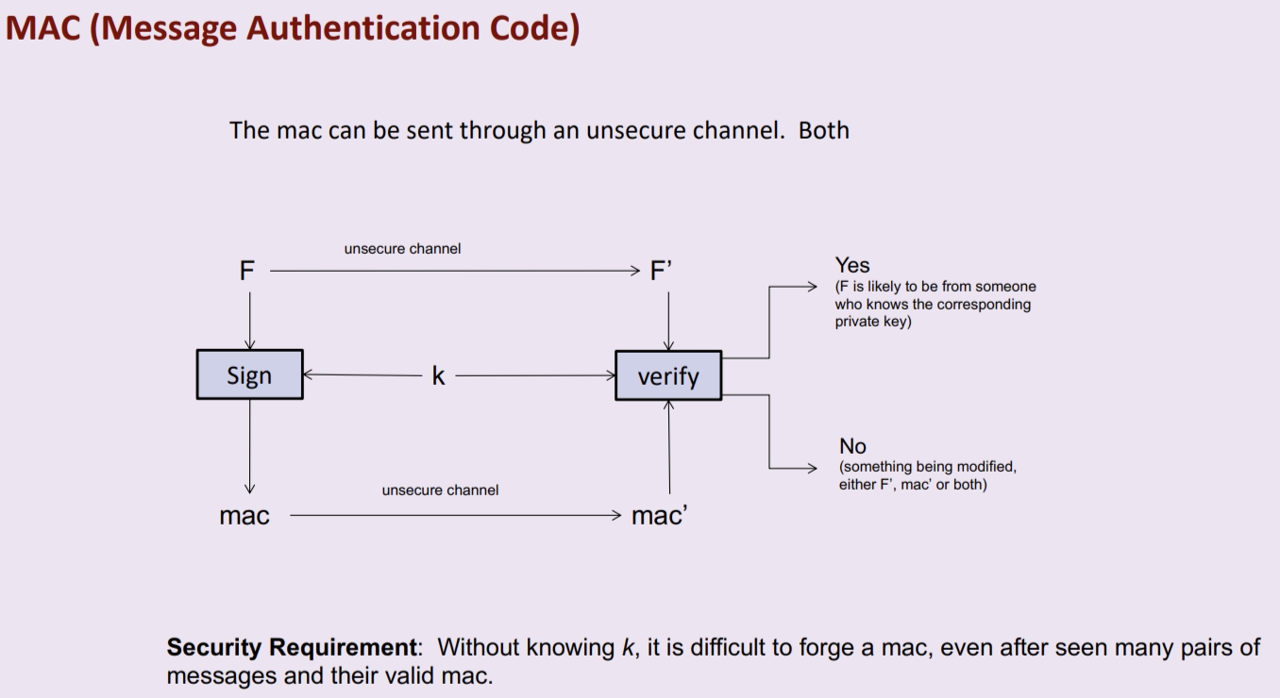
\includegraphics[width=1\linewidth]{authSummary2}}
\null
\centerline{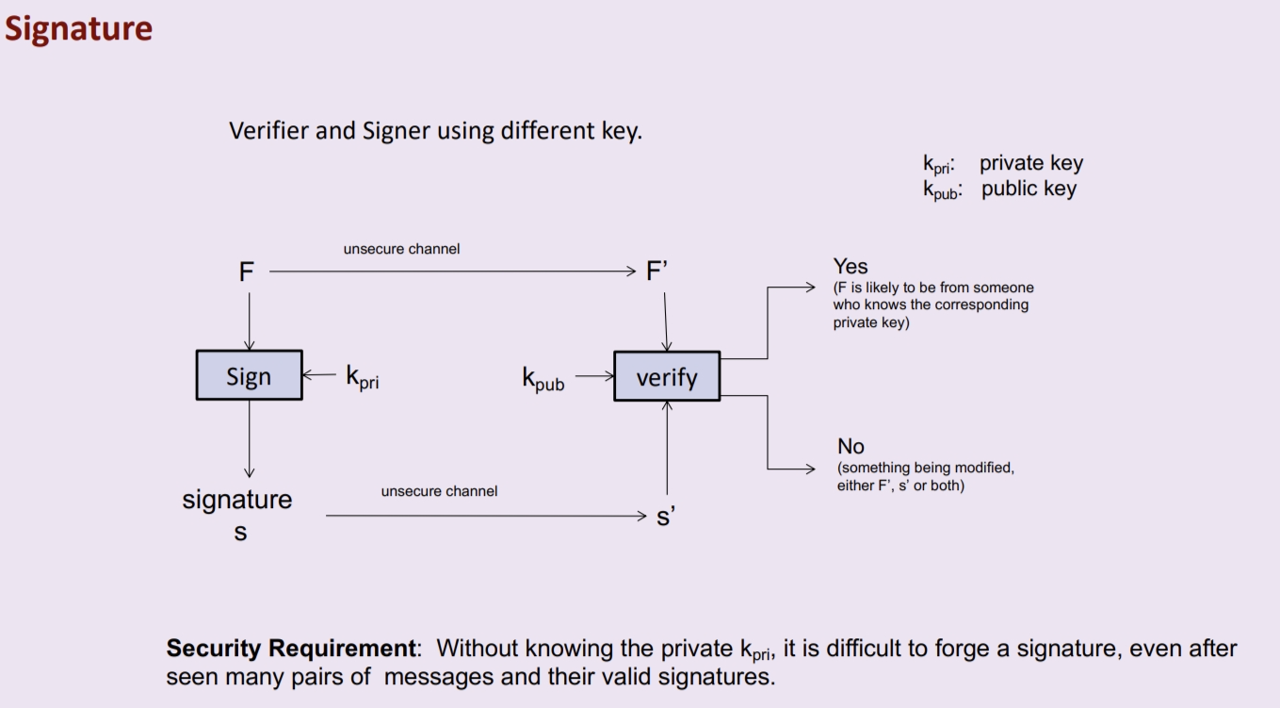
\includegraphics[width=1\linewidth]{authSummary3}}

\vfill \null

\columnbreak

\subsection{3.2 Data Authenticity (Hash): Unkeyed Hash}
\textbf{Follow Kerckhoff's Principle}: Adversary knows all the algorithms.

\subsubsection{Hash}
\begin{itemize}
\item \textbf{A (cryptographic) hash} is a function that takes an arbitrary large message as input, and 
outputs a fixed size (say 160 bits) digest.
\item \textbf{Collision-resistant}:It is difficult for an attacker to find two different messages m1 , m2 that “hash” to the same digest.
\item \textbf{One-way}:  A hash that is collision-resistant is also one-way, that is, given a digest d, it is difficult to find a 
message m s.t. $h(m)=d$.
\item Examples of non-secure hash algorithms: (taking selected bits from data, CRC checksum).
\item \textbf{Popular Hash}: 
	\begin{itemize}
	\item \textbf{SHA-0, SHA-1/2/3}: SHA-1 popular standard producing 160-bits message digest, employed in SSL, SSH etc. In 2017, successful collision attack on SHA-1 found.
	\item \textbf{MD5}: Produces 128-bit digest. However, algorithm that can find collisions have been found.
	\end{itemize}
\end{itemize}

\subsubsection{Application Scenario of Unkeyed Hash (no secret keys)}
\begin{itemize}
\item \textbf{Example:} Alice downloaded a software vlc-2.2.8-win32.exe from the web. Is the downloaded file authentic?
\item Since the website is hosted with HTTPS protocol, Alice is being assured that the content displayed on the
browser is from VLC and authentic.
\item However, the downloading site is a 3rd-party, channel not secure. Possibility 3rd party website is malicious and giving out virus infested software.
\item To verify that the file indeed original, after download, check the integrity by matching the “hash” of the file with the “SHA-256 checksum” displayed in the browser. If they match, file is intact. If not, file is corrupted.
\end{itemize}
\centerline{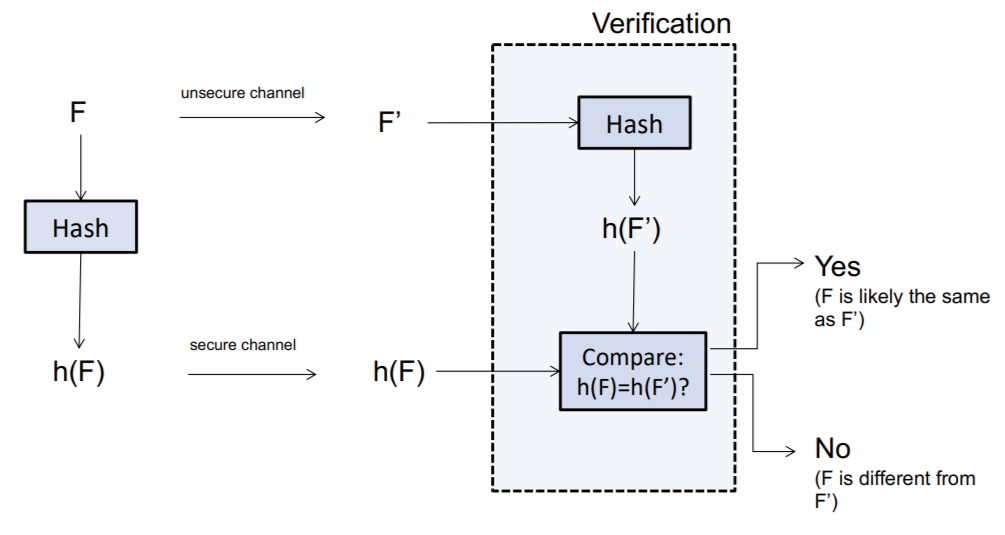
\includegraphics[width=0.7\linewidth]{unkeyedHash}}

\begin{itemize}
\item For the attacker, to find a $F'$ that has the same hash as F, this is known as \textbf{2nd preimage problem}.
\item Although practically, some part of program needs to be same to be workable, we focus on modest goal of finding any file. If easiest goal preventable, so is harder goal. Hence, for hash, \textbf{easiest attack goal is ``collision''}.
\item \textbf{A Hash function H() is called collision-resistant} if it is computationally difficult to 
solve collision attack. More specifically, it is collision-resistant if no method can 
significantly outperform birthday attack
\end{itemize}

\columnbreak

\subsection{3.3 Data Authenticity (MAC): Keyed Hash}
\begin{itemize}
\item \textbf{MAC}: Message Authentication Code.
\item \textbf{A keyed-hash} is a function that takes an arbitrary large message and a \textbf{secret key} as 
input, and outputs a fixed size (say 160 bits) MAC.
\item \textbf{Forgery-resistant}: Even with multiple valid pairs of messages and mac, difficult for attacker to forge the mac of 
message not seen before.
\item \textbf{Popular Keyed-Hash (MAC)}
	\begin{itemize}
	\item \textbf{CBC-MAC}: (based on AES under CBC mode)
	\end{itemize}
\centerline{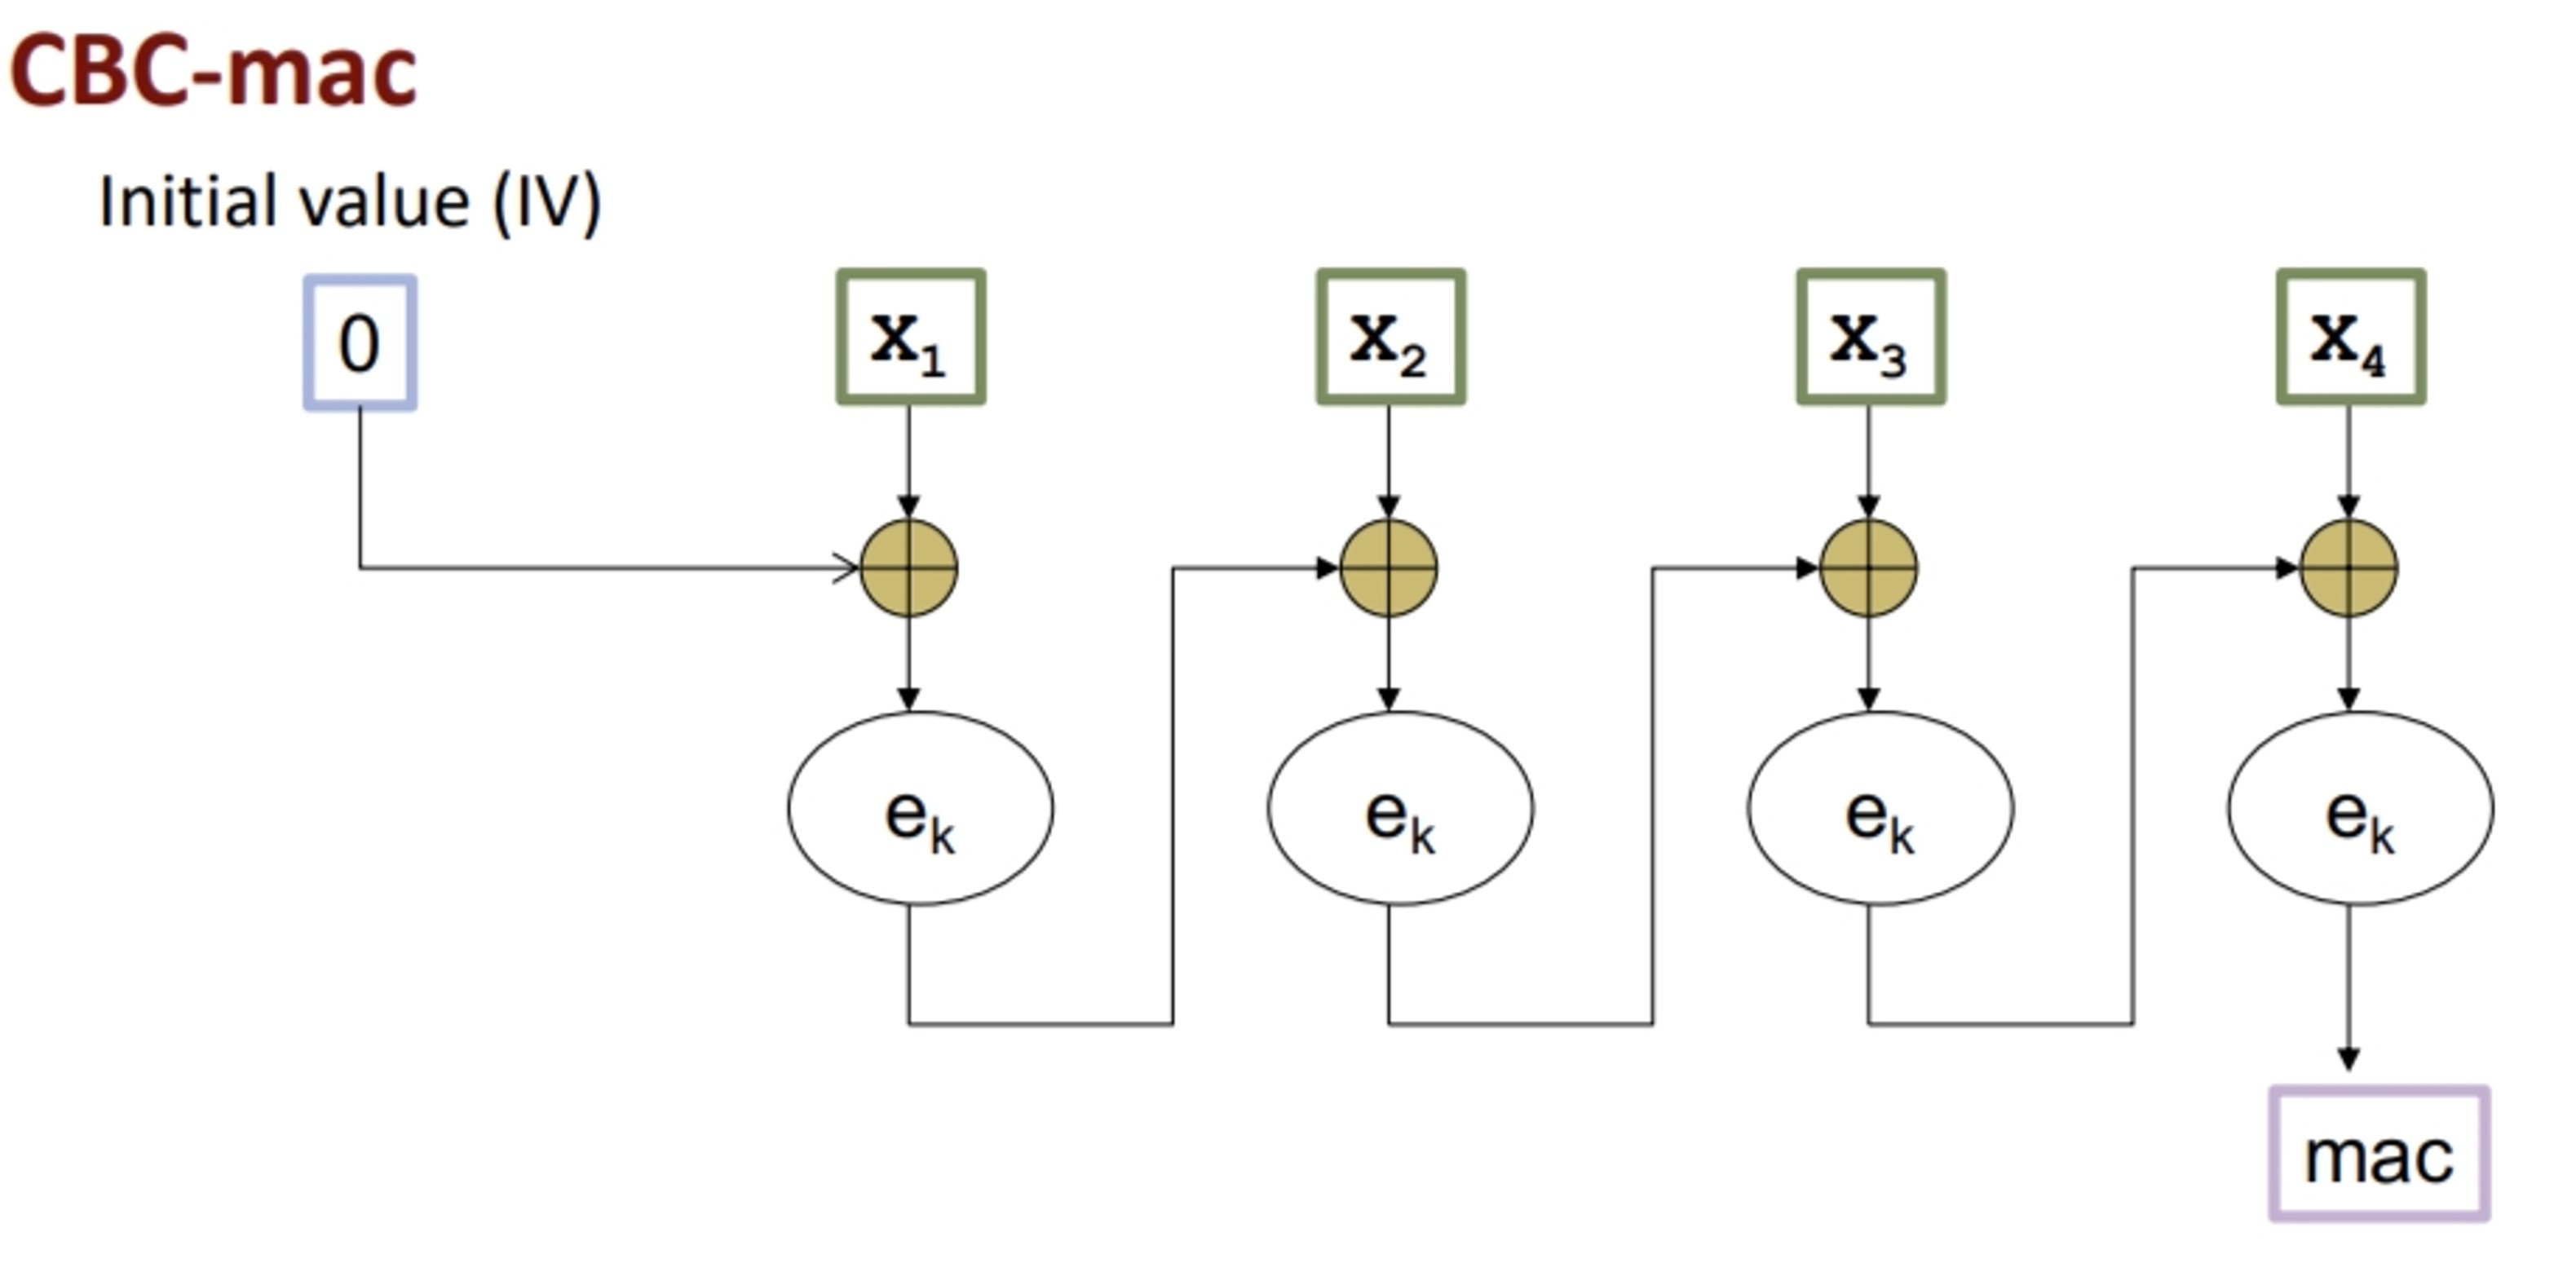
\includegraphics[width=0.7\linewidth]{CBCMac}}
	\begin{itemize}
	\item \textbf{HMAC} : based on SHA (optional)
	\end{itemize}
\end{itemize}

\subsection{Application Scenario for MAC (keyed hash)}
\begin{itemize}
\item In the previous example (on vlc), we assume secure channel to send the digest.
\item In scenarios without secure channel to deliver the digest, we can protect the digest with the help of some secrets. 
	\begin{itemize}
	\item In the symmetric key setting, it is called the mac.
	\item In the public key setting, it is called the digital signature
	\end{itemize}
\end{itemize}
\centerline{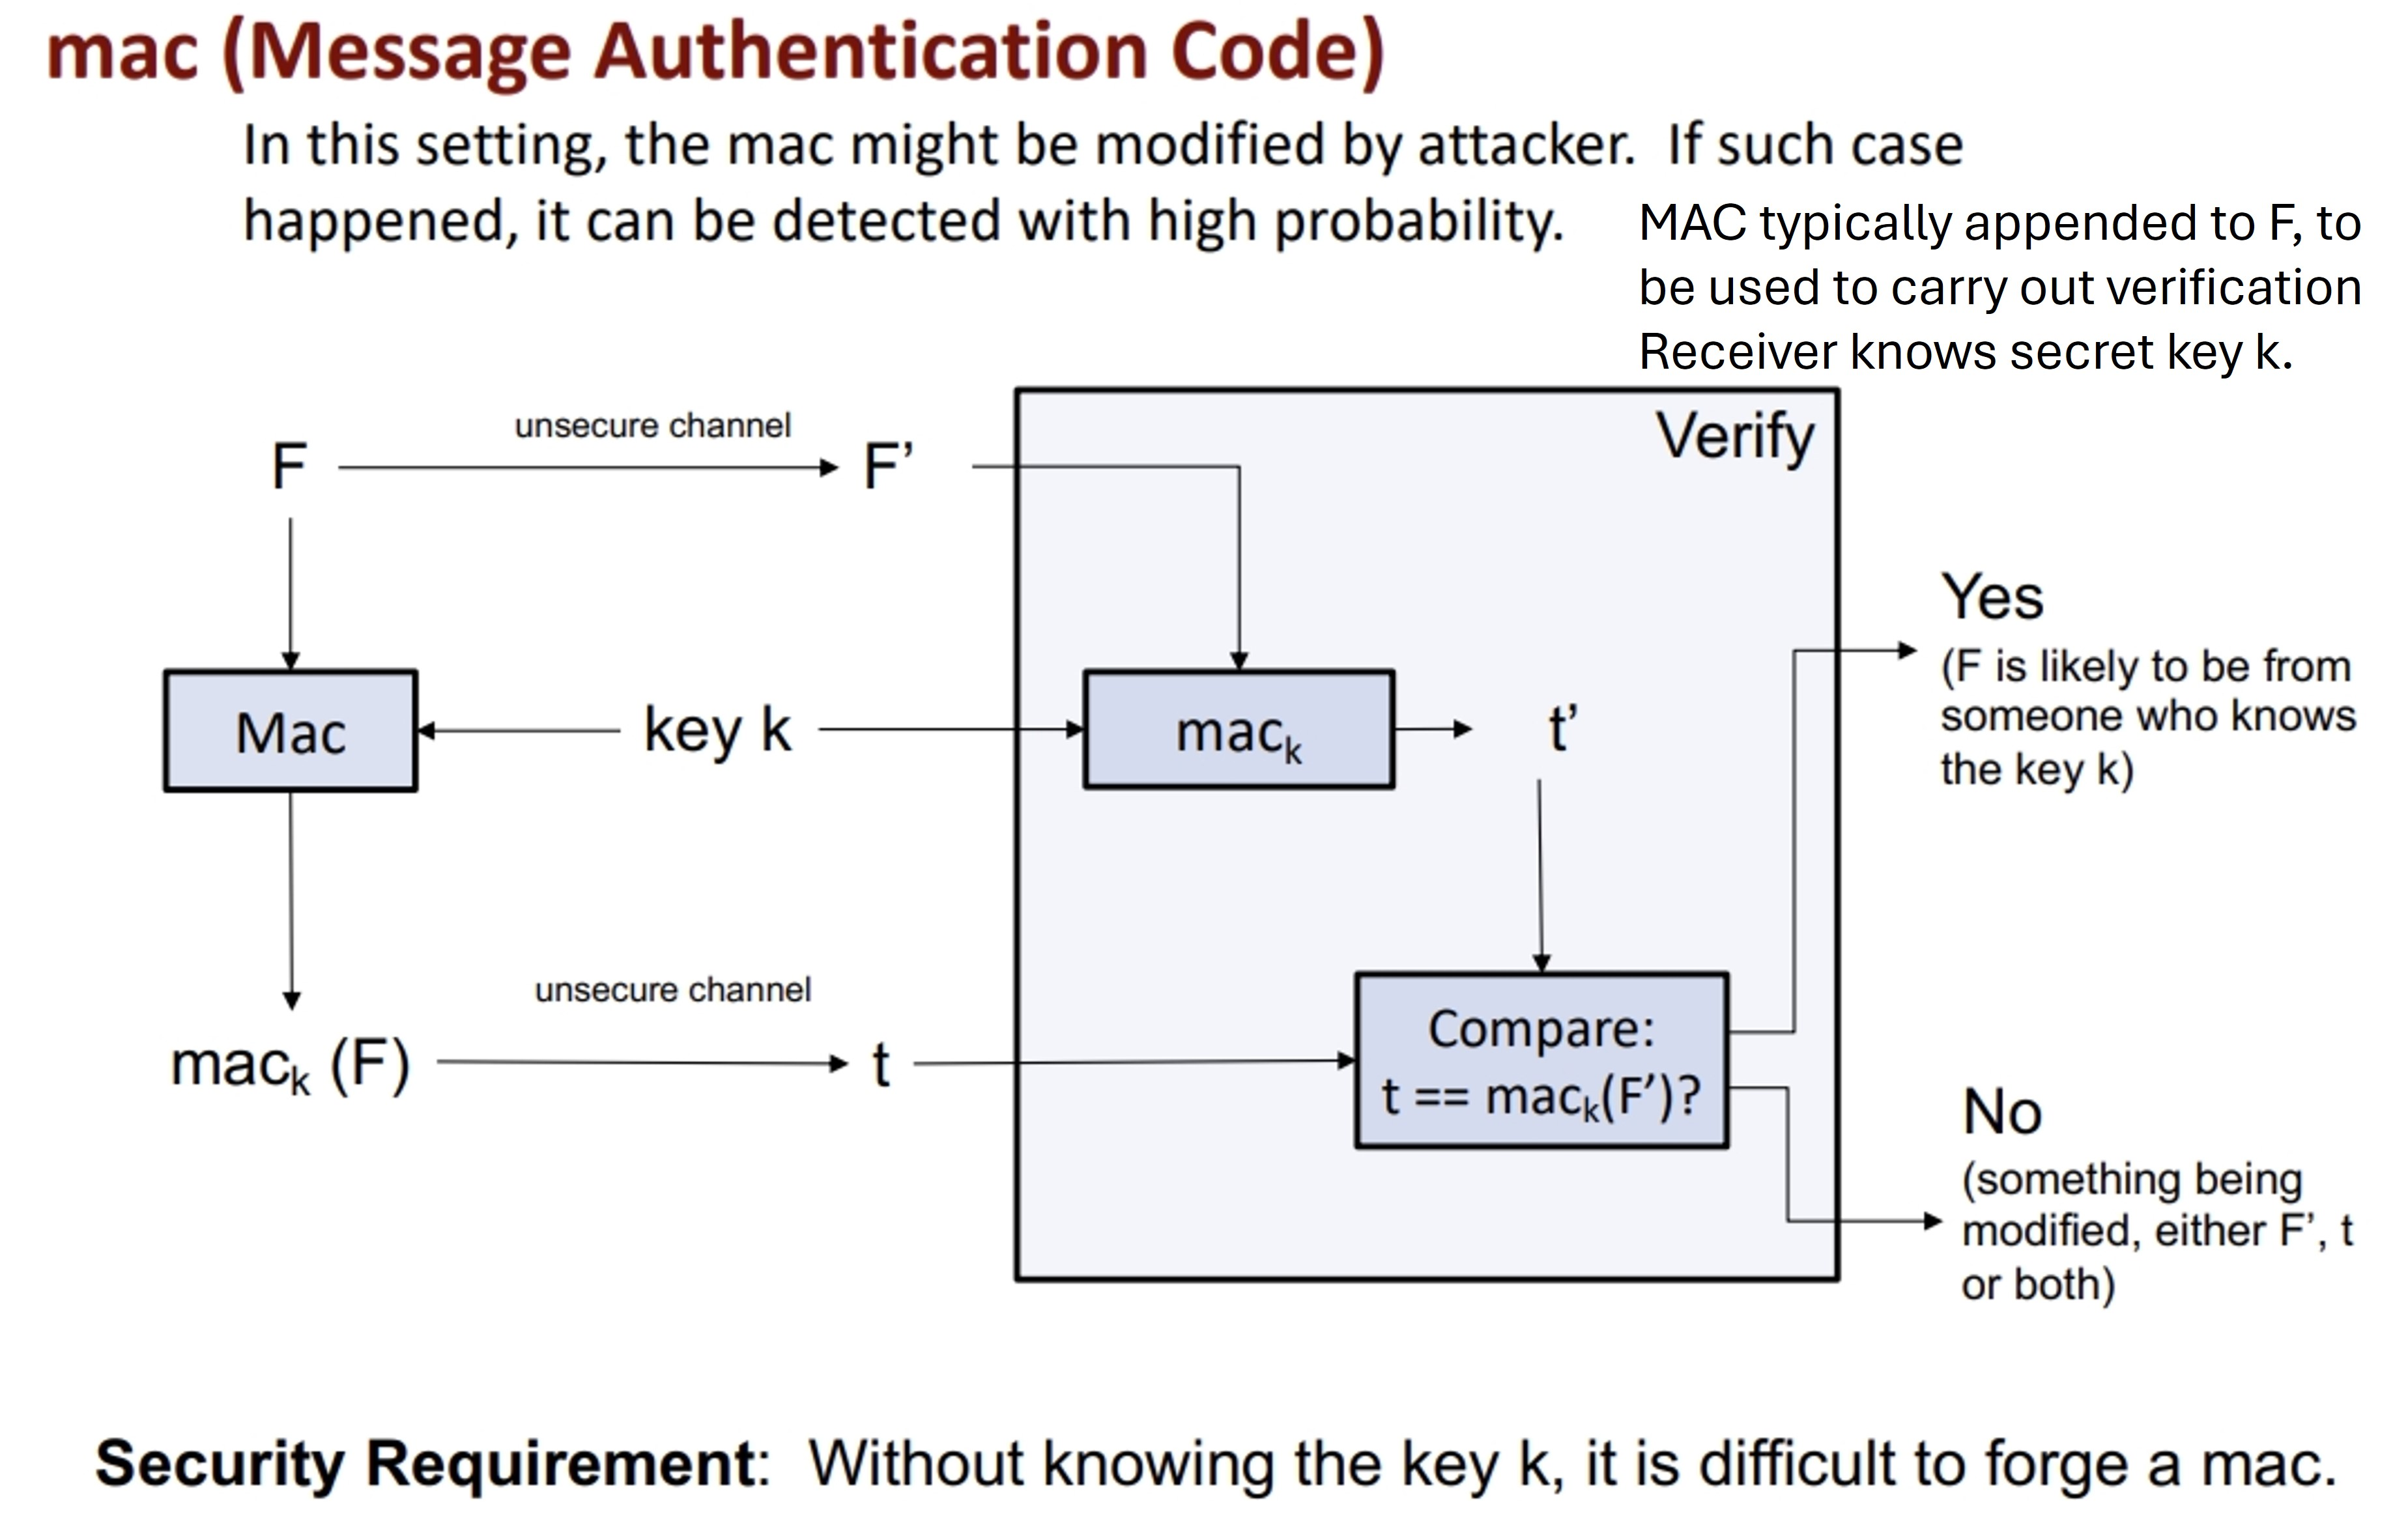
\includegraphics[width=0.9\linewidth]{MACusecase}}	
\begin{itemize}
\item Attacker would need to forge valid pair of (message, mac).
\item Typically, the mac is appended to F. Stored as a single file / transmitted together. (Aka authentication tag / code). Later, entity can carry out the verification process using secret key. 
\end{itemize}

\null
\null\null\null
\columnbreak

\subsection{3.4 Data Authenticity (Signature): Asymmetric Key}
\textbf{Public Key Version of MAC is called Signature}

\begin{itemize}
\item Here, the owner uses the private key to generate the signature. The public can
use the public key to verify the signature.
\item So, anyone can verify the authenticity of the data, but only the person who know
the private key can generate the signature.
\end{itemize}

\centerline{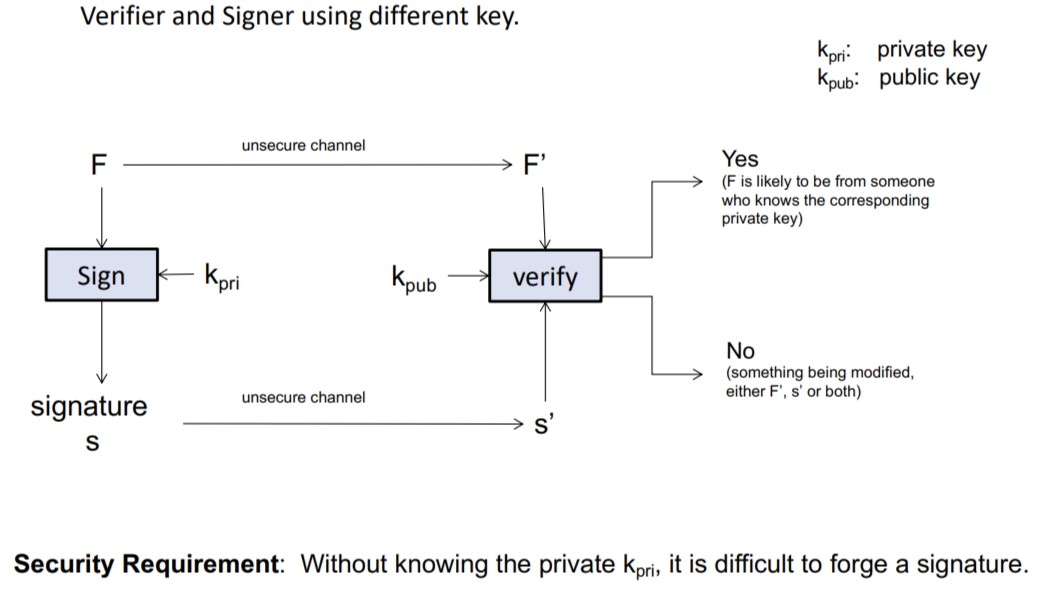
\includegraphics[width=0.9\linewidth]{Signature}}	

\begin{itemize}
\item Similarly, computed signature appended to F and stored as a single file.
\item ``Alice signs file F'': signature is computed using Alice's private key and F, then appended to F.
\item \textbf{Authenticity'} of F can be verified by anyone, using the public key. The valid signature 
can only be computed by someone who knows the private key. So, if it is valid, then F must be 
authentic. 
\item \textbf{Non-repudiation}:  Assurance that someone cannot deny previous commitments or 
actions.
\item	Can be seen as digital signature, certified authentic, on top of ease of key management.
\item \textbf{Popular Signature Scheme}:
	\begin{itemize}
	\item A popular group of schemes use RSA for the sign/verify component: RSASSA-PSS, RSASSA-PKCS1: signature scheme based on RSA
	\item DSA (Digital Signature Algorithm) is another popular standard whose security
depends on discrete log.
	\end{itemize}
\end{itemize}

\subsubsection{Design of Signature Scheme}
\textbf{Signature} need two things: \textbf{Unkeyed hash,  sign/verify algorithm}.
\centerline{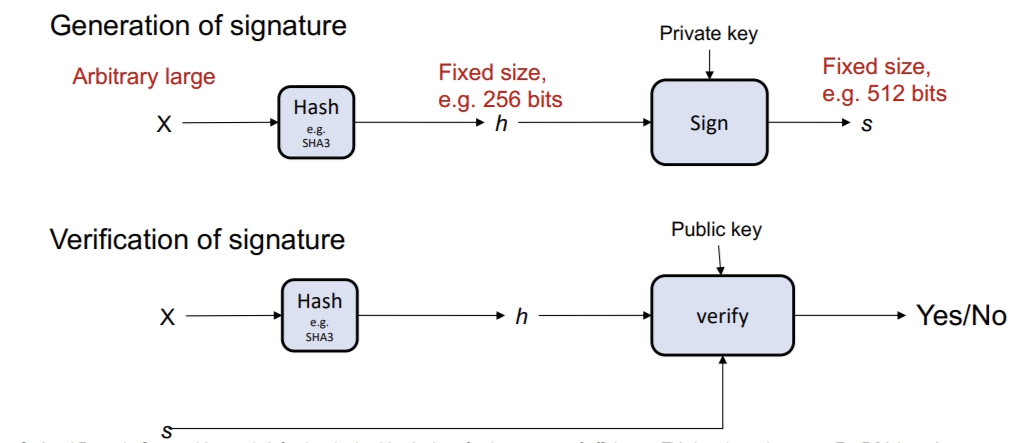
\includegraphics[width=0.9\linewidth]{signatureScheme}}	
\begin{itemize}
\item Hashing done not only for purpose of efficiency.
\item For RSA-based signature, to be secure, hash must be carried out, e.g. if message very short, only 1 byte.
\item For RSA, essentially, signature is the ``encrypted'' digest. During verification, decrypt to obtain digest and compare.
\item \textit{Note}: Here, we use private key to encrypt. Previously, we used public key to encrypt. Role flipped.
\end{itemize}


\subsection{3.5 Attacks \& Pitfalls}

\subsection{Birthday Attack on hash}
Similar to ``exhaustive search'' in encryption. Birthday attack applicable to all hash functions, similar to how exhaustive search is on all encryption schemes.

\begin{itemize}
\item Hashes are designed to be \textbf{collision-resistant}, hard to find two diff. messages give same digest. However, subjected to birthday attack.
\item We want to design a hash so that known attacks cannot do better than birthday attack.
\item \textbf{Birthday attack} is an attack that occurs when someone exploits the mathematics behind the birthday problem in probability theory to launch a cryptographic attack. 
\item The birthday problem states that in a group of 23 people, there's a 50\% chance that at least two will have the same birthday.
\end{itemize}

\subsubsection{Birthday Attack Formula (Single Common Pool)}
\begin{itemize}
\item Suppose we have \textbf{$M$ messages}.
\item Each value tagged with value randomly chosen, range of values = [1, T]. \textbf{($T$ is no. of values)}
\item \textbf{If}:
\end{itemize}
\centerline{$M > 1.17 * T^{0.5}$}
\begin{itemize}
\item There is a probability higher than 0.5 that there is a pair of messages tagged with the same value.
\item i.e. \textbf{$P$(collision) $>$ 0.5}.
\end{itemize}
\centerline{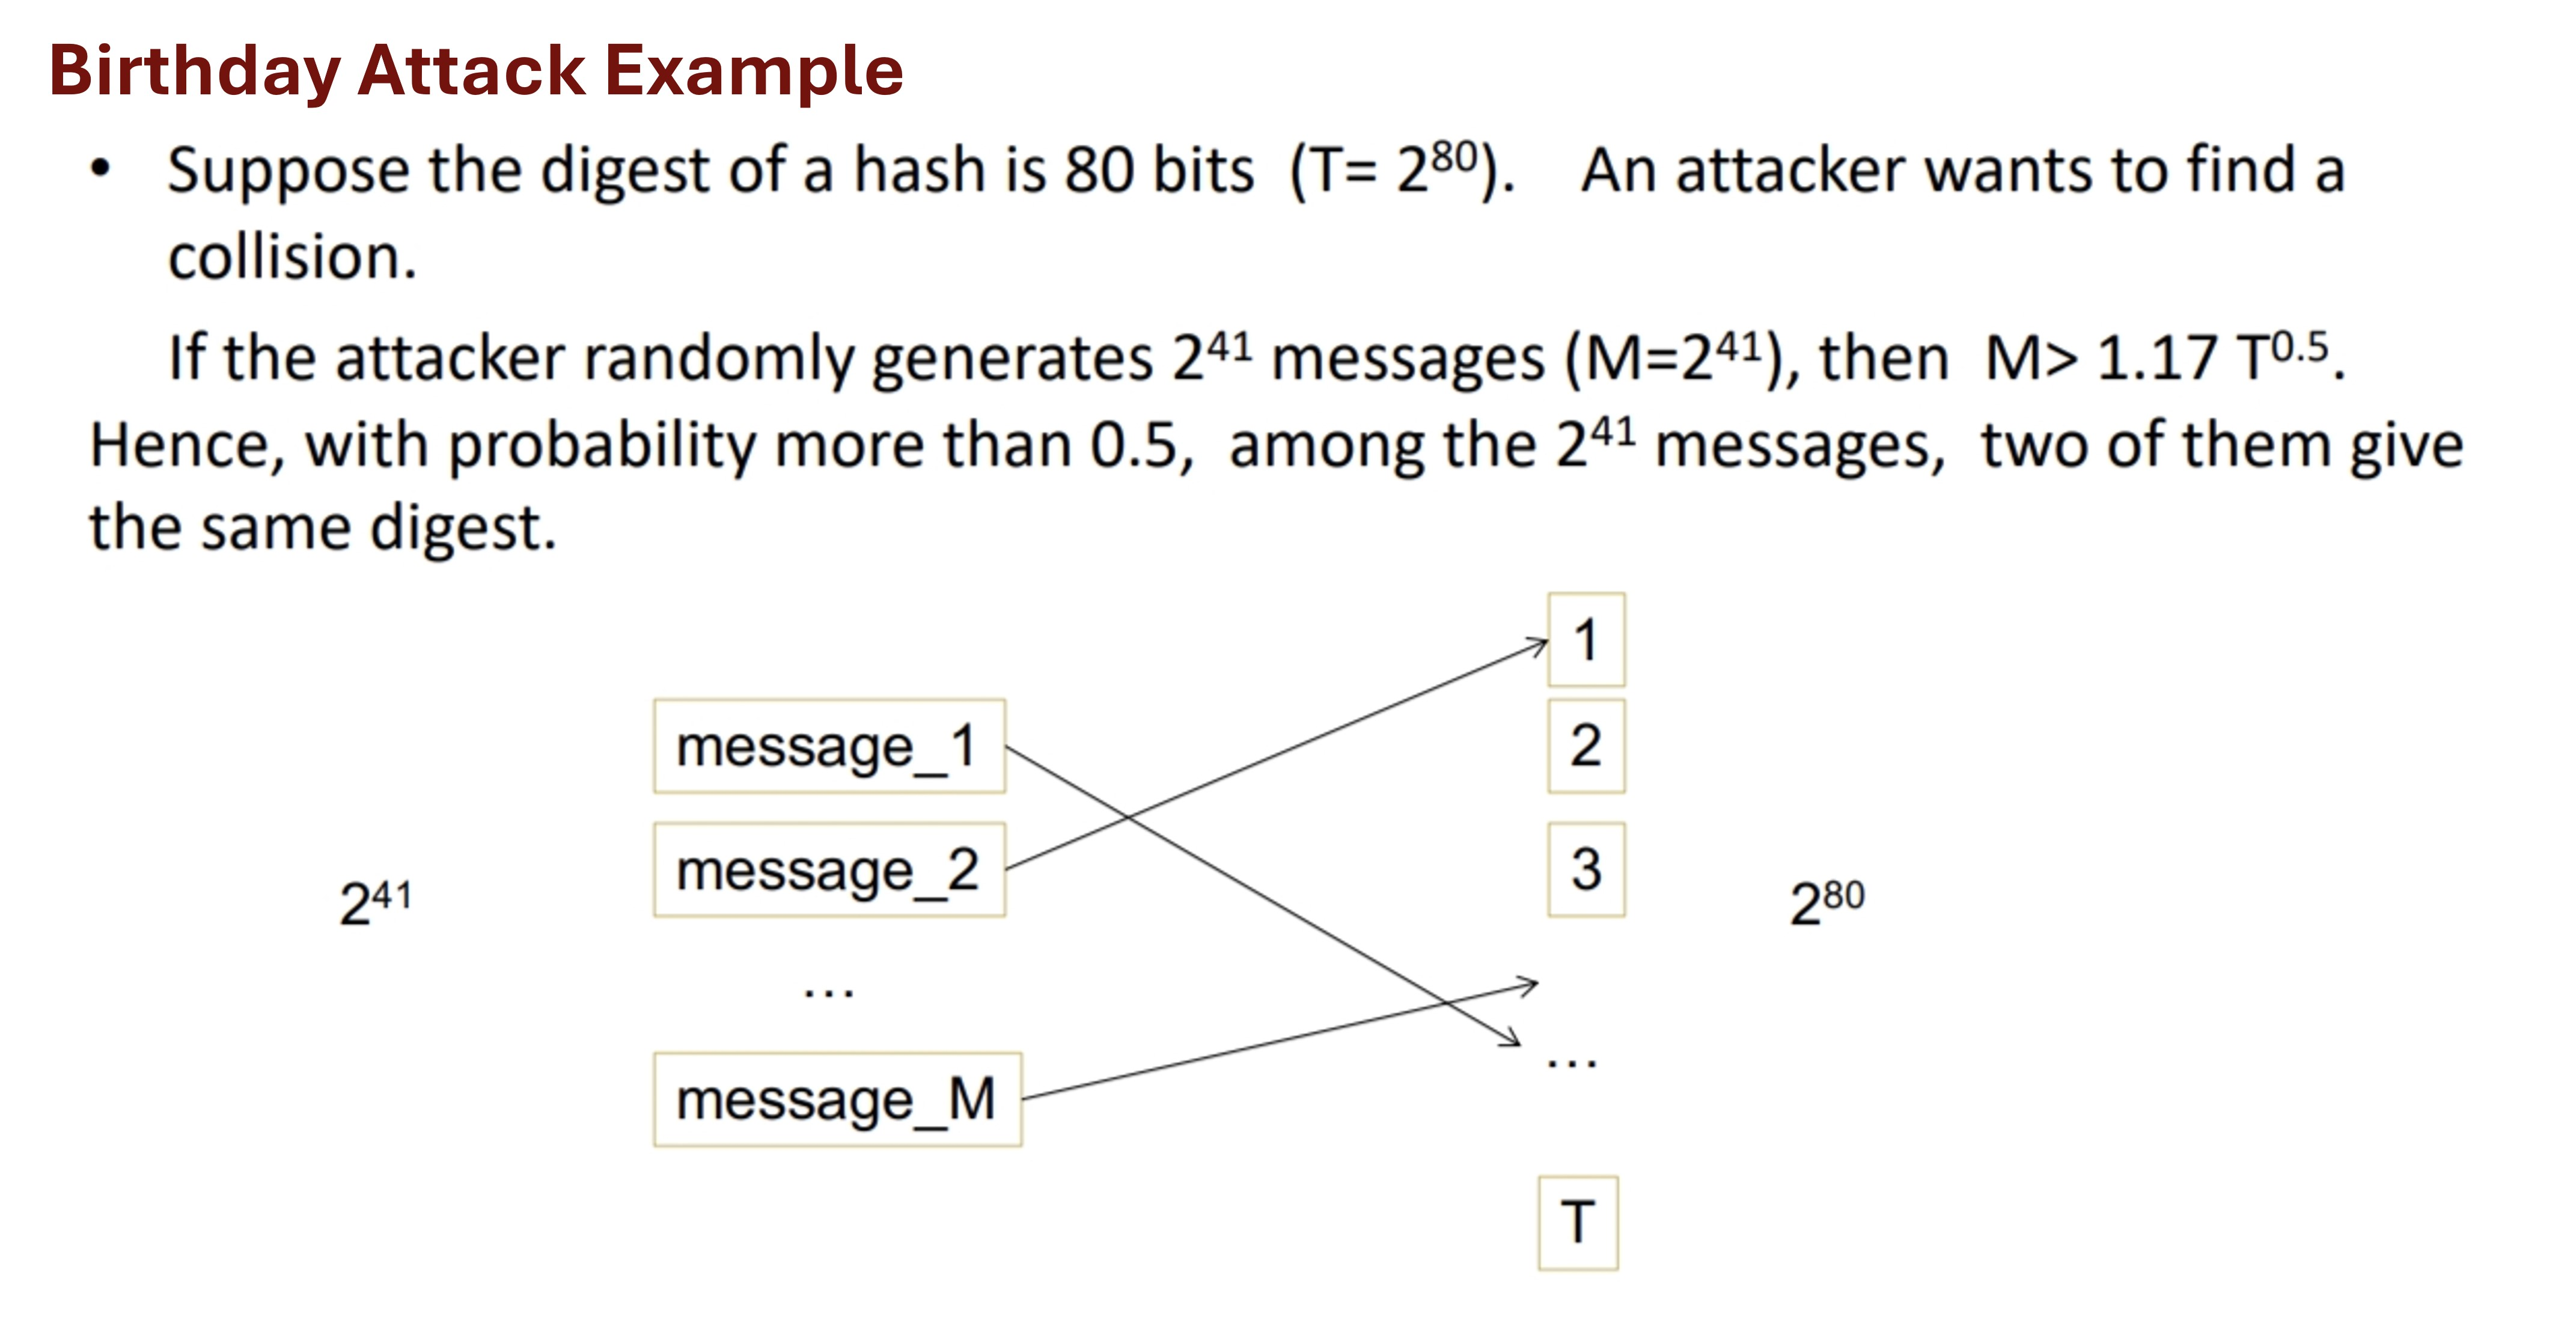
\includegraphics[width=1\linewidth]{birthdayAttack}}
\begin{itemize}
\item In general, for a \textbf{set of $T$ values}, where \textbf{$M$ values chosen randomly},
\item the probability \textbf{at least one value chosen more than once} (aka collision) approximately:
\end{itemize}
\centerline{$ p(M;T)\approx 1-e^{-M(M-1)/(2T)}$}
\smallskip
\centerline{$\approx 1-e^{-M^{2}/(2T)}$}
\begin{itemize}
\item NIST recommendation of key length: (2019-2030) \\
Security Strength (key length for symmetric key): 112 \\
Discrete Logarithm Key (length of digest): 224.
\item The length of truncated message digests used shall be at least twice the desired security
strength required for the digital signature. (Due to birthday attack)
\end{itemize}

\subsubsection{Variant of Birthday Attack (Two Pools)}
The first version in lecture notes takes a pair from a common pool.
\begin{itemize}
\item Consider where there are two pools. One item in the pair is drawn from a pool, and another item drawn from another pool.
\item Let $S$ be a set of $k$ distinct elements where each element is an $n$ bits
binary string. Now, let us independently and randomly select a set $T$
of $m$ $n$-bit binary strings.
\item It can be shown that, the probability that
$S$ has non-empty intersection with $T$ is more than
\end{itemize}
\centerline{$1 - 2.7^{-km2^{-n}}$}


\subsection{3.6 Additional Notes}
\subsection{3.6.1 Design flaw: Using encryption for authenticity}
\begin{itemize}
\item Encryption is designed to provide confidentiality. It does not necessary guarantee 
integrity and authenticity. 
\item In example, XYZ wants to achieve “authenticity”, but wrongly employed encryption to achieve that. (Some encryption schemes also provide authenticity, but not all.)
\item Note that a lot of details are omitted. Simply adding mac to the instructions is not sufficiently secure. To prevent 
“replay” attack, “nonce” is required. Essentially, problem is about authenticity a communicating party, not just authenticating the data source. Hence a secure implementation would employ TLS (to be covered) first, and then send the instruction via TLS. Secure but less efficient.
\end{itemize}

\subsection{3.6.2 Password Vs. Secret Key in Crypto}
\begin{itemize}
\item Passwords are generated by human to be remembered by humans.
\item Secret keys (e.g. 128-bit AES encrypt key, 1024-bit RSA key) machine generated, truly random, or derived based on data.
\item However, sometimes password used as source for secret key. (E.g. use password to encrypt file). 
\item Transformation is called \textbf{key derivation function}, (KDF)
\end{itemize}


\subsection{3.6.3 Hash Application: (Password file protection)}
\begin{itemize}
\item Password file stores userid, password. 
\item This file could be leaked (insider / accidental leakage, hack). Many well-known incidents where weak/unprotected password files leak, large number of passwords compromise. Desirable to add additional layer of protection on file. (See 2.1).
\item \textbf{Password file should be ``hashed'' and ``salted''}.
\item During authentication, password entered is hashed, and compared with value stored in password file.
\item \textbf{Salt is important}: If no attacker can just hash a common password, and check to see if it matches any of the 100,000 leaked passwords. Salt (not secret) forces attacker to test one by one.
\item Due to one-way property of hash, password file if leaked, is not as disasterous.
\end{itemize}

\null \null \null
\columnbreak

\vfill\null
\columnbreak 

\section{4. PKI and Channel Security}

\subsection{PKI and Channel Security Summary}
\centerline{\includegraphics[width=1\linewidth]{PKISummary}}	
\smallskip
\centerline{\includegraphics[width=1\linewidth]{PKISummary2}}	

\section{4.1 Public Key Distribution}
In order to use digital signature (compared to symmetric key, or unkeyed digest, or MAC, which require some secret key between sender and receiver), we still need a \textbf{secure way for receiver to obtain sender's public key}.

\subsubsection{Why require Public Key Distribution?}
\begin{itemize}
\item While both need secure channel to distribute keys, it is easier to securely ``broadcast'' public key than to ``establish'' different symmetric key for every pair.
\item With public key distributed, can use for encryption (\textbf{confidentiality}) and signature verification (\textbf{authenticity}).
\item \textbf{Public Key}: Entity broadcasts public key to public billboard only once, and no need know existence of receiver while broadcasting.
\item \textbf{Symmetric Key}: Entity needs different symmetric key per pair, and both entities need to interact to establish key.
\end{itemize}

\subsubsection{Key Distribution Methods}
\begin{itemize}
\item Public Announcement on existing mechanism (social media, name card)
\item Hard coded in verification programs
\item Publish in publicly available directory
\item Public Key Infrastructure (PKI)
\end{itemize}

First few solutions have potential issues. How to verify information submitted is authentic, not everyone trusts the server, server may be overwhelmed, cannot handle load. Hence, \textbf{PKI} as a distributed way to broadcast the keys.

\columnbreak

\section{4.2 Public Key Infrastructure (PKI)}

PKI is a standardized system that distribute public keys. To address limitation of the previous 
methods. \\
A main objective is to be deployable on a large scale. 
\begin{itemize}
\item \textbf{Two main components}: \textbf{Certificate}, and \textbf{Chain of trust of Certificate Authority (CA)}.
\item “Public PKI” refer to the PKI we adopted in Internet for domain name, emails address etc. In short,  “PKI”. 
\item “Private PKI” are systems for other applications, has own set of “CA”. (E.g. possible for company to set up a PKI for own usage).
\end{itemize}

\subsection{4.2.1 Certificate Authority (CA)}
\begin{itemize}
\item  \textbf{CA} is a trusted authority that manages a directory of public keys, issues certificates. An entity can request to add its public key. CA also has its \textbf{own public-private key}. 
\item Anyone can send queries to search the directory. (Certificates facilitate checking/querying to be done in an offline manner.)
\item Assume some CA’s public keys securely distributed via other means. (so, we still need a secure channel to distribute the CA’s public key, e.g. pre-loaded in OS, known as ``root CAs'').
\item Not all
CAs’ public keys are preloaded. Other CA’s public keys can be added through the chain-of-trust.
\end{itemize}

\subsection{4.2.2 Certificate }
\begin{itemize}
\item \textbf{Certificate} simply document signed by CA, containing an identity, associated public key, valid time window, and signature of CA. It binds the public key to the identity, and is certified by the signature.
\item \textbf{Rationale: Certificate for distributing public keys}:
\begin{itemize}
\item `Lazy CA'': A certificate is simply a precomputed ``reply''. CA ``signs'' message beforehand, and pass to sender, and sender sends this signed message to receiver. This is called the certificate.
\item Since no one except CA can produce the valid signature, authenticity of information in certificate as good as coming directly from the CA.
\end{itemize}
\item \textbf{A certificate} is a digital document that contains at least the following 4 main items:
	\begin{enumerate}
	\item The name(s), for e.g. alice@yahoo.com or bbc.com or *.bbc.com (note that *.bbc.com is a set of names)
	\item The public key of the owner.
	\item The time window that this certificate is valid. (Expiry)
	\item The signature of the CA
	\end{enumerate}
\item \textbf{Other important info:} 
	\begin{itemize}
	\item Usage of certificate (type of name email or domain name, whether name can take role of a CA (chain of trust))
	\item Digest (Fingerprint), for verification without using CA's public key
	\item Meta data such as algo involved in verifying signature. (E.g. ECC / RSA, key length)
	\end{itemize}
\item Hence, from certificate, receiver can obtain sender's public key, and verify authenticity without connection to CA. 
\item \textbf{Assumption}: Receiver trusts CA.
\item \textbf{Standard}: E.g. ITU-T X.509 standardisation body, specifies format for certificates, certificate revocation lists, validation algorithm.
\item Self-signed certificate by a CA is also called “root-certificate”
\end{itemize}

\columnbreak

\subsection{4.2.3 Certificate Authority \& Trust Relationship}
\begin{itemize}
\item \textbf{Reponsibility of CA}: CA needs to verify information is correct, which could be costly. Getting certificate signed by reputable CA is not free.
\item \textbf{Certificate Chain-of-trust}: There might be too many CAs. Root CA (preloaded public key) to CA\#1, to CA\#2 etc. is called \textbf{chain of trust}.
\end{itemize}

\subsection{4.2.4 Certificate Revocation}
\begin{itemize}
\item Non-expired certificates may be revoked due to different reasons: 
	\begin{itemize}
	\item Private key compromised, vulnerability in choosing key, admin left organization, Business entity closed, Issuing CA compromised. 
	\end{itemize}
\item Verifier needs to check if certificate is still valid, although the certificate not expired yet. (conflicting requirement!!)
\item \textbf{Two different approaches to certificate revocation:}
	\begin{itemize}
	\item \textbf{Certificate Revocation List (CRL)}: CA periodically signs and publishes a revocation list. Need an online CRL Distribution Point.
	\item \textbf{Online Certificate Status Protocol (OCSP)}: OCSP Responder validates a cert in question. Need an online OCSP Responder.
	\end{itemize}
\item Recommendation is for a user (e.g. browser) to periodically (say weekly) update its local cache of revocation list. The user does not need to online check whenever the user wants to verify a certificate.
\end{itemize}

\section{4.3 Limitations/Attacks on PKI}

\subsection{4.3.1 Implementation Bugs}
\begin{itemize}
\item Same as many other secure designs, it is vulnerable if not implemented correctly
\item \textbf{E.g.} Some browsers ignore substrings after null characters when displaying in address bar but include them when verifying certificate. (ww.nus.sg\textbackslash0.hacker123.com $\rightarrow$ displayed as www.nus.sg). Viewer thought connected via https to a, but in fact connected to b).
\end{itemize}

\subsection{4.3.2 Abuse by CA}
\begin{itemize}
\item Many CA’s. One could be malicious. Rogue CA can forge any cert.
\item \textbf{E.g.}: Trustwave issue man-in-middle digital cert, Lenovo's SuperFish scandal.
\end{itemize}

\subsection{4.3.3 Social Engineering}
\begin{itemize}
\item Social engineering exploits \textbf{confusing naming convention}, so that the verifiers are tricked into using a wrong name.
\item E.g, an attacker first rightfully registered for a domain name that resembles a targeted domain name. Next, used the registered domain to confuse the victim in phishing attack. 
\item A few techniques to confuse the verifier: “Domain typosquatting”, “Homograph attack”, using sub-domain name. These attack are aka Domain spoofing, URL spoofing, Fake URL, etc
\item \textbf{Typosquatting}: Register for domain name (e.g. one letter off), employ phishing attack. Rely on typos made by users when inputting website address, lead to any URL.
\item \textbf{Sub-Domain}: E.g. rightful owner of 123.com can get sub.domain nus.edu.sg.123.com (*.123.com) 
\end{itemize}




\section{Authentication Protocols}
Consider 3 types of protocols: (basic) authentication, key-exchange, authenticated key-exchange. 
\begin{itemize}
\item \textbf{Attack Model}: Attack-then-impersonate
\item \textbf{Types:} Unilateral, Mutual
\item \textbf{Authentication Method:} Challenge-response
\end{itemize}

\section{4.4. (basic) Authentication Protocol}
\centerline{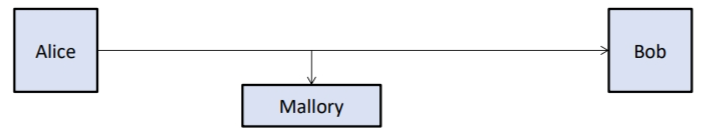
\includegraphics[width=0.8\linewidth]{basicAuth}}	
\begin{itemize}
\item \textbf{Scenario}: Entity wants to convince Bob that she is indeed Alice. The entity does so by convincing Bob that she knows some “secrets”.
\item \textbf{Attack Model}: Attack-then-impersonate. Attacker (Mallory) can sniff and modify the communication between the authentic Alice and 
Bob. Attacker uses stolen info to impersonate Alice. Can simply \textbf{"replay"} password sent to impersonate.
\end{itemize}

\subsection{Authentication: Challenge-reponse}
Suppose Alice and Bob have a shared secret $k$, both agreed on a message authentication code (MAC). An entity who knows $k$ is either Alice or Bob. Entity P
wants to convince Alice that he is Bob. (P: “Prover”).
\begin{enumerate}
\item P sends to Alice a hello message.
\item \textbf{Challenge}: Alice randomly picks message $m$ and sends $m$ to $P$.
\item \textbf{Response}: $P$ computes $t = mac_k(m)$. $P$ sends $t$ to Alice.
\item Alice verifies tag received is indeed mac of $m$. If so, accept, else reject.
\end{enumerate}
\begin{itemize}
\item By property of \textbf{mac}, even if Eve (third party) sniff communication and obtain multiple pairs of valid $m$, $t$, Eve still (1) can’t get the secret key $k$, (2) can’t forge the mac for messages that Eve has not seen before!
\item Eve can’t replay response as challenge randomly chosen, likely different in next authentication session. Challenge $m$ ensures \textbf{freshness} of authentication process. It is also known as the cryptographic \textbf{nonce}.
\item This protocol only authenticates Bob. That is, authenticity of Bob is verified. Hence, called \textbf{unilateral authentication}. There are also protocols to verify both parties, which are called mutual authentication.
\end{itemize}

\subsection{Authentication: Challenge-reponse using PKC}
Public key version using signature (Unilateral Authentication). Alice wants to authenticate entity $P$ who claims to be Bob.
\begin{enumerate}
\item (Challenge) Alice chooses a random message $r$ and sends to $P$: (“Bob, here is your challenge”, r)
\item (Response) P uses his private key to sign $r$. P also attaches a certificate: (sign(r), certificate)
\item Alice verifies certificate belongs to Bob and valid. Next, extracts public key from certificate and verify signature sign(r) is correct. If so, accept.
\end{enumerate}
\begin{itemize}
\item If Alice already knows Bob’s public key, the certificate can be omitted.
\item Assume Attacker observes multiple interactions. By security property of signature, eavesdropper cannot derive Bob’s private key, can’t forge response.
\item Nonce r ensure freshness. 
\end{itemize}


\section{4.5 Key-exchange}
Two communicating entities want to establish a shared key between them. Consider attack Eve who can sniff, goal to steal established key.

\subsection{PKC-based Key-exchange}
\centerline{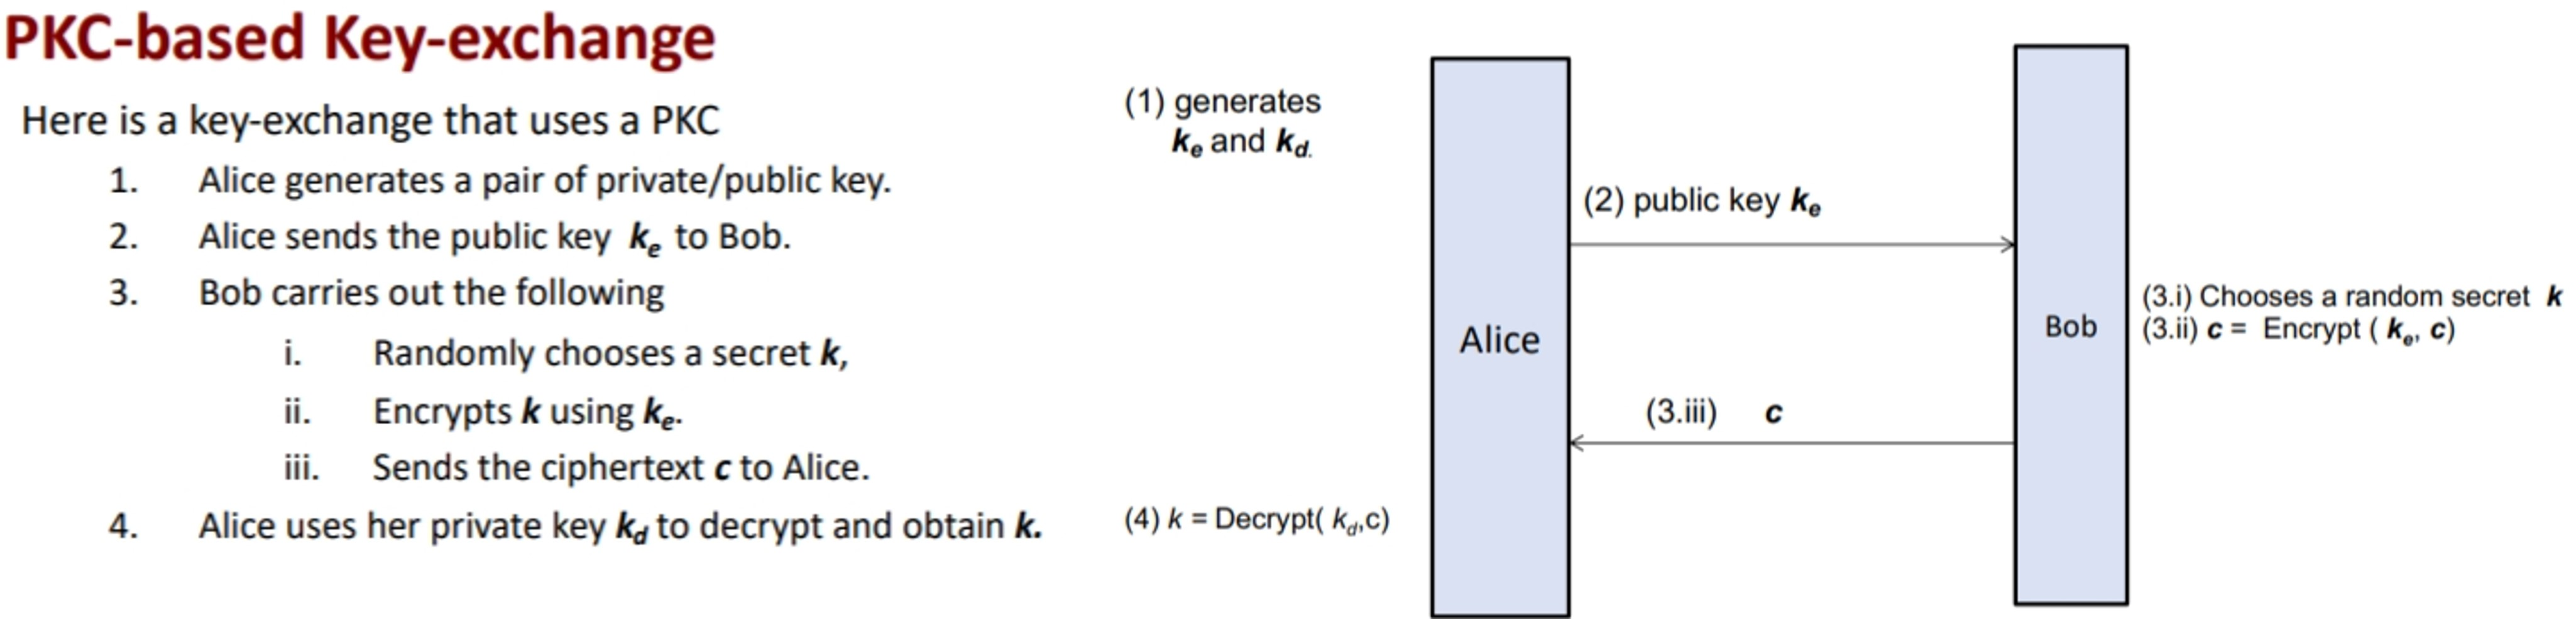
\includegraphics[width=1\linewidth]{PKCKeyExchange}}	
\begin{itemize}
\item Attacker (Eve) can only obtain the public key $k_e$ and the ciphertext $c$.
\item By security of PKC, from the public and ciphertext, attacker can’t get any information of the plaintext, which is the key $k$.
\end{itemize}

\subsection{Diffie-Hellman Key-exchange}
\centerline{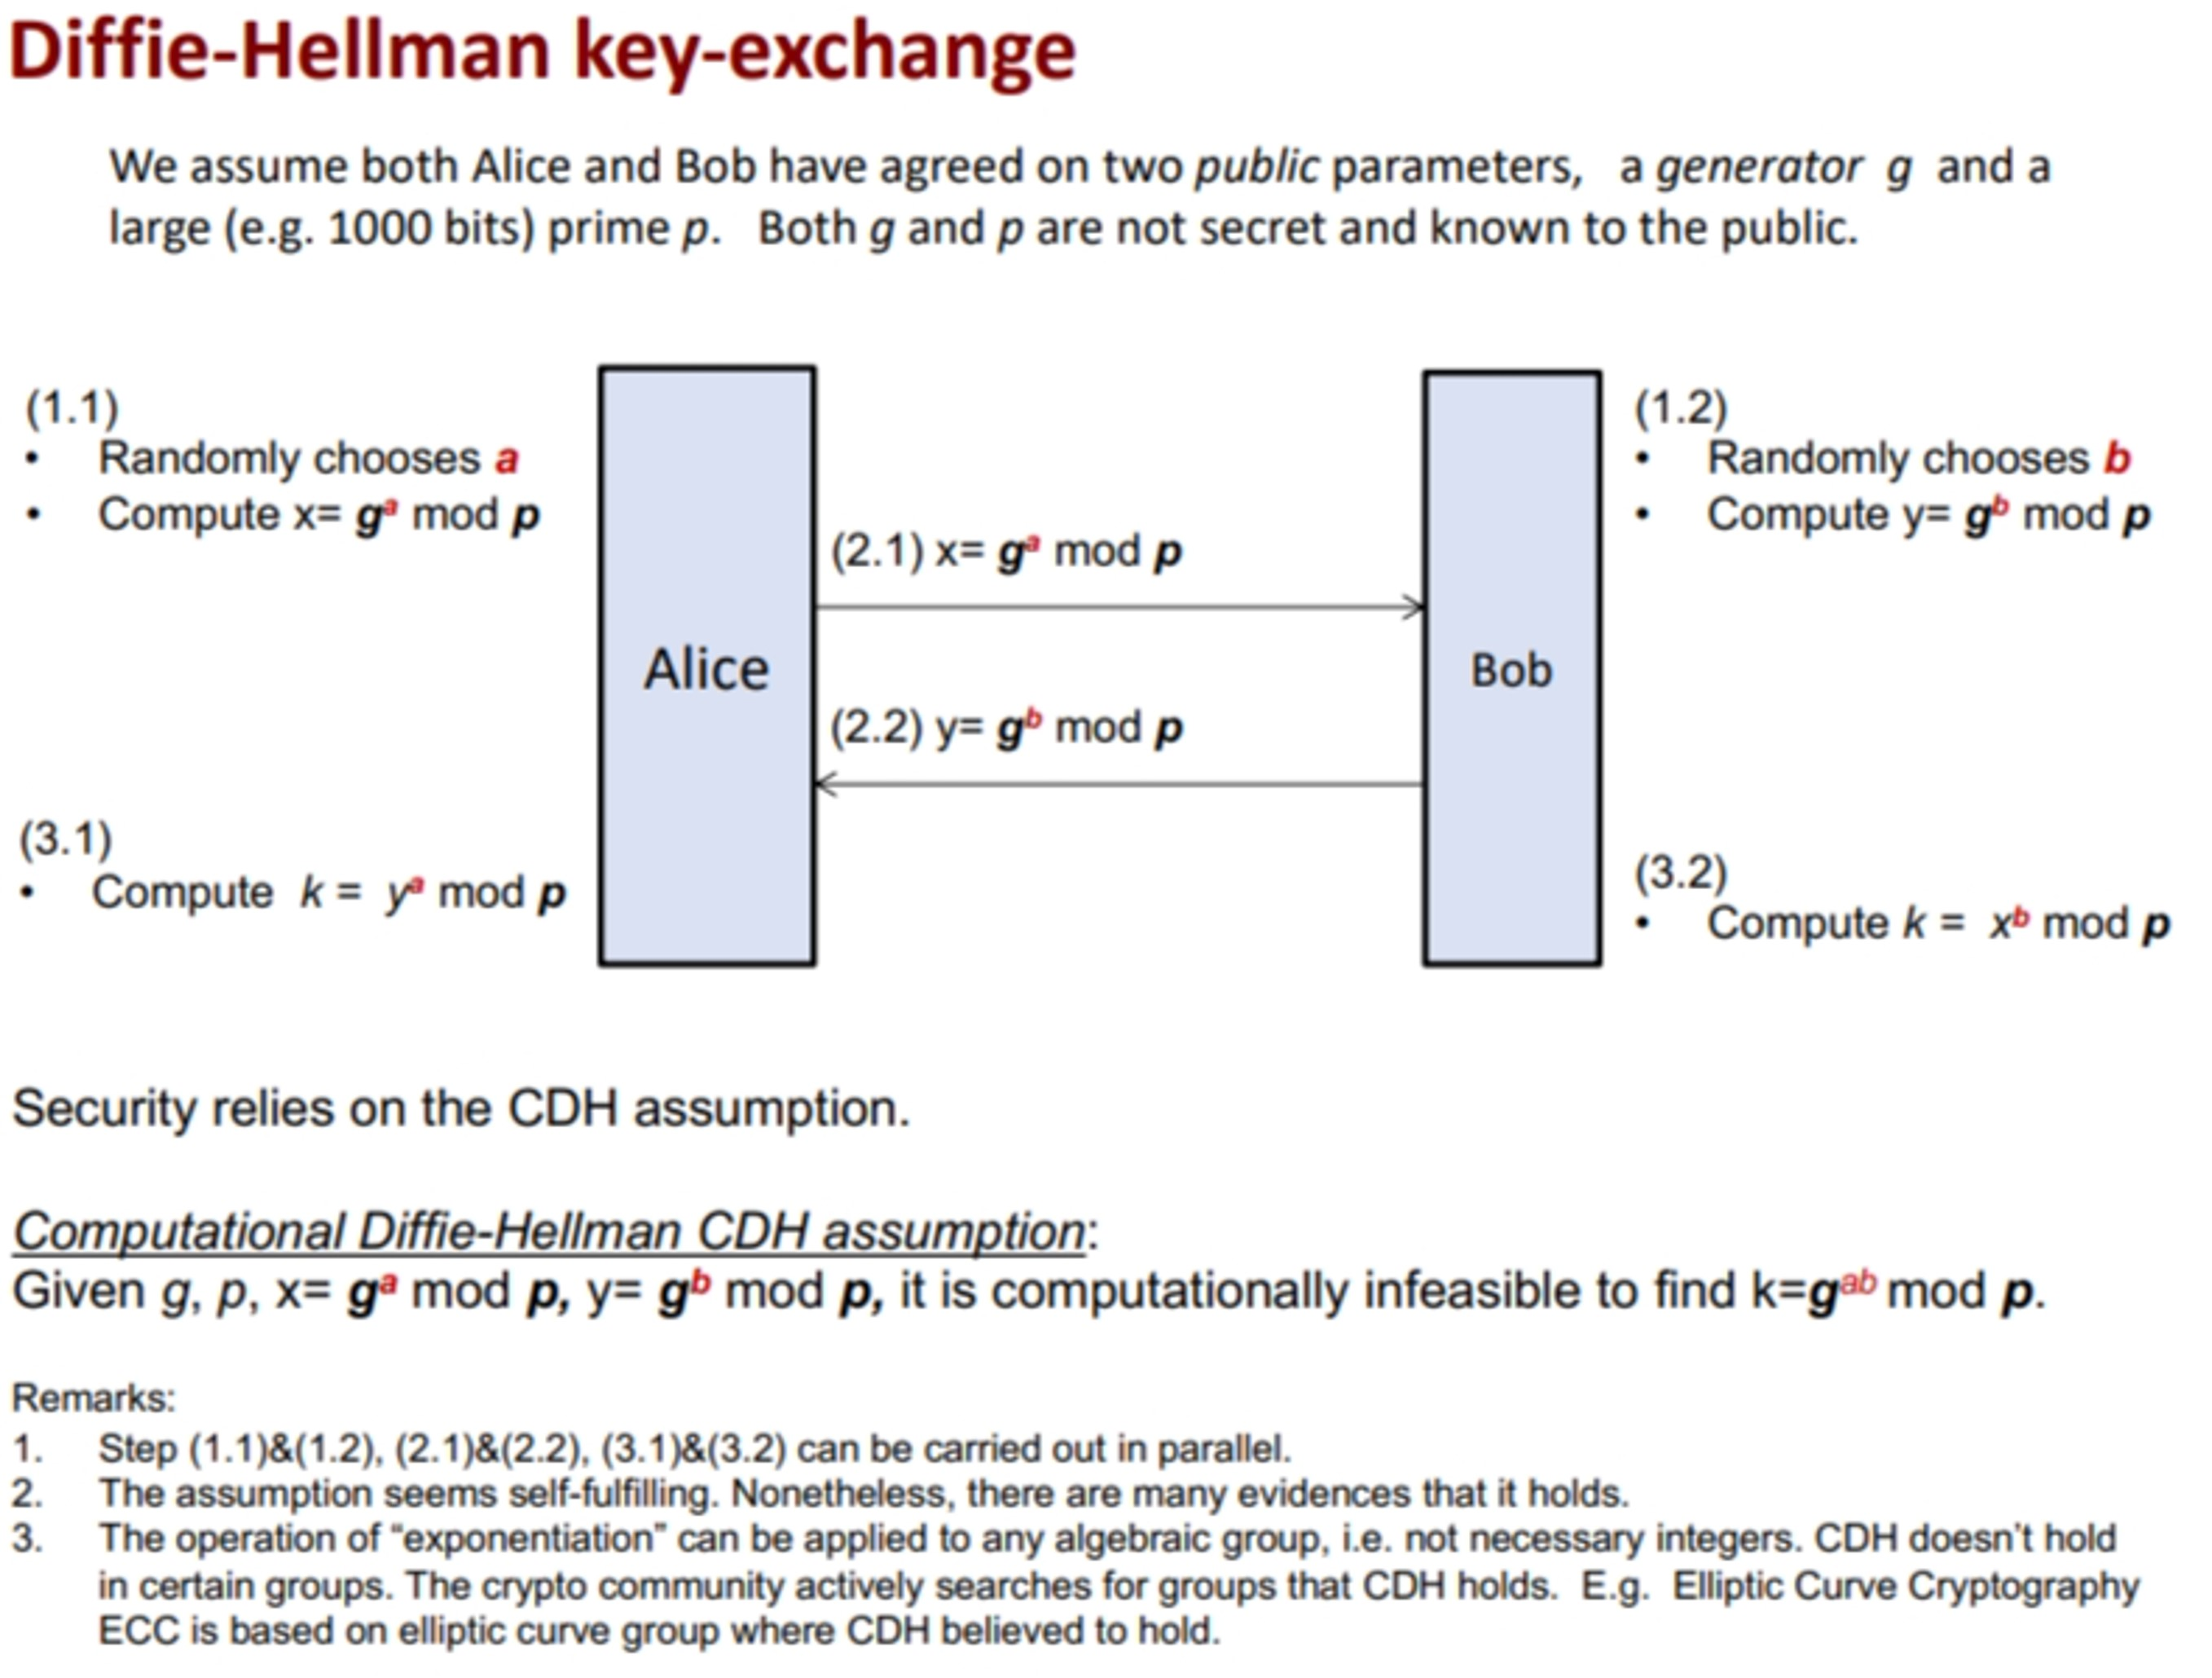
\includegraphics[width=1\linewidth]{DHKeyExchange}}	
\medskip
\subsubsection{Diffie-Hellman Key-exchange Example}
\centerline{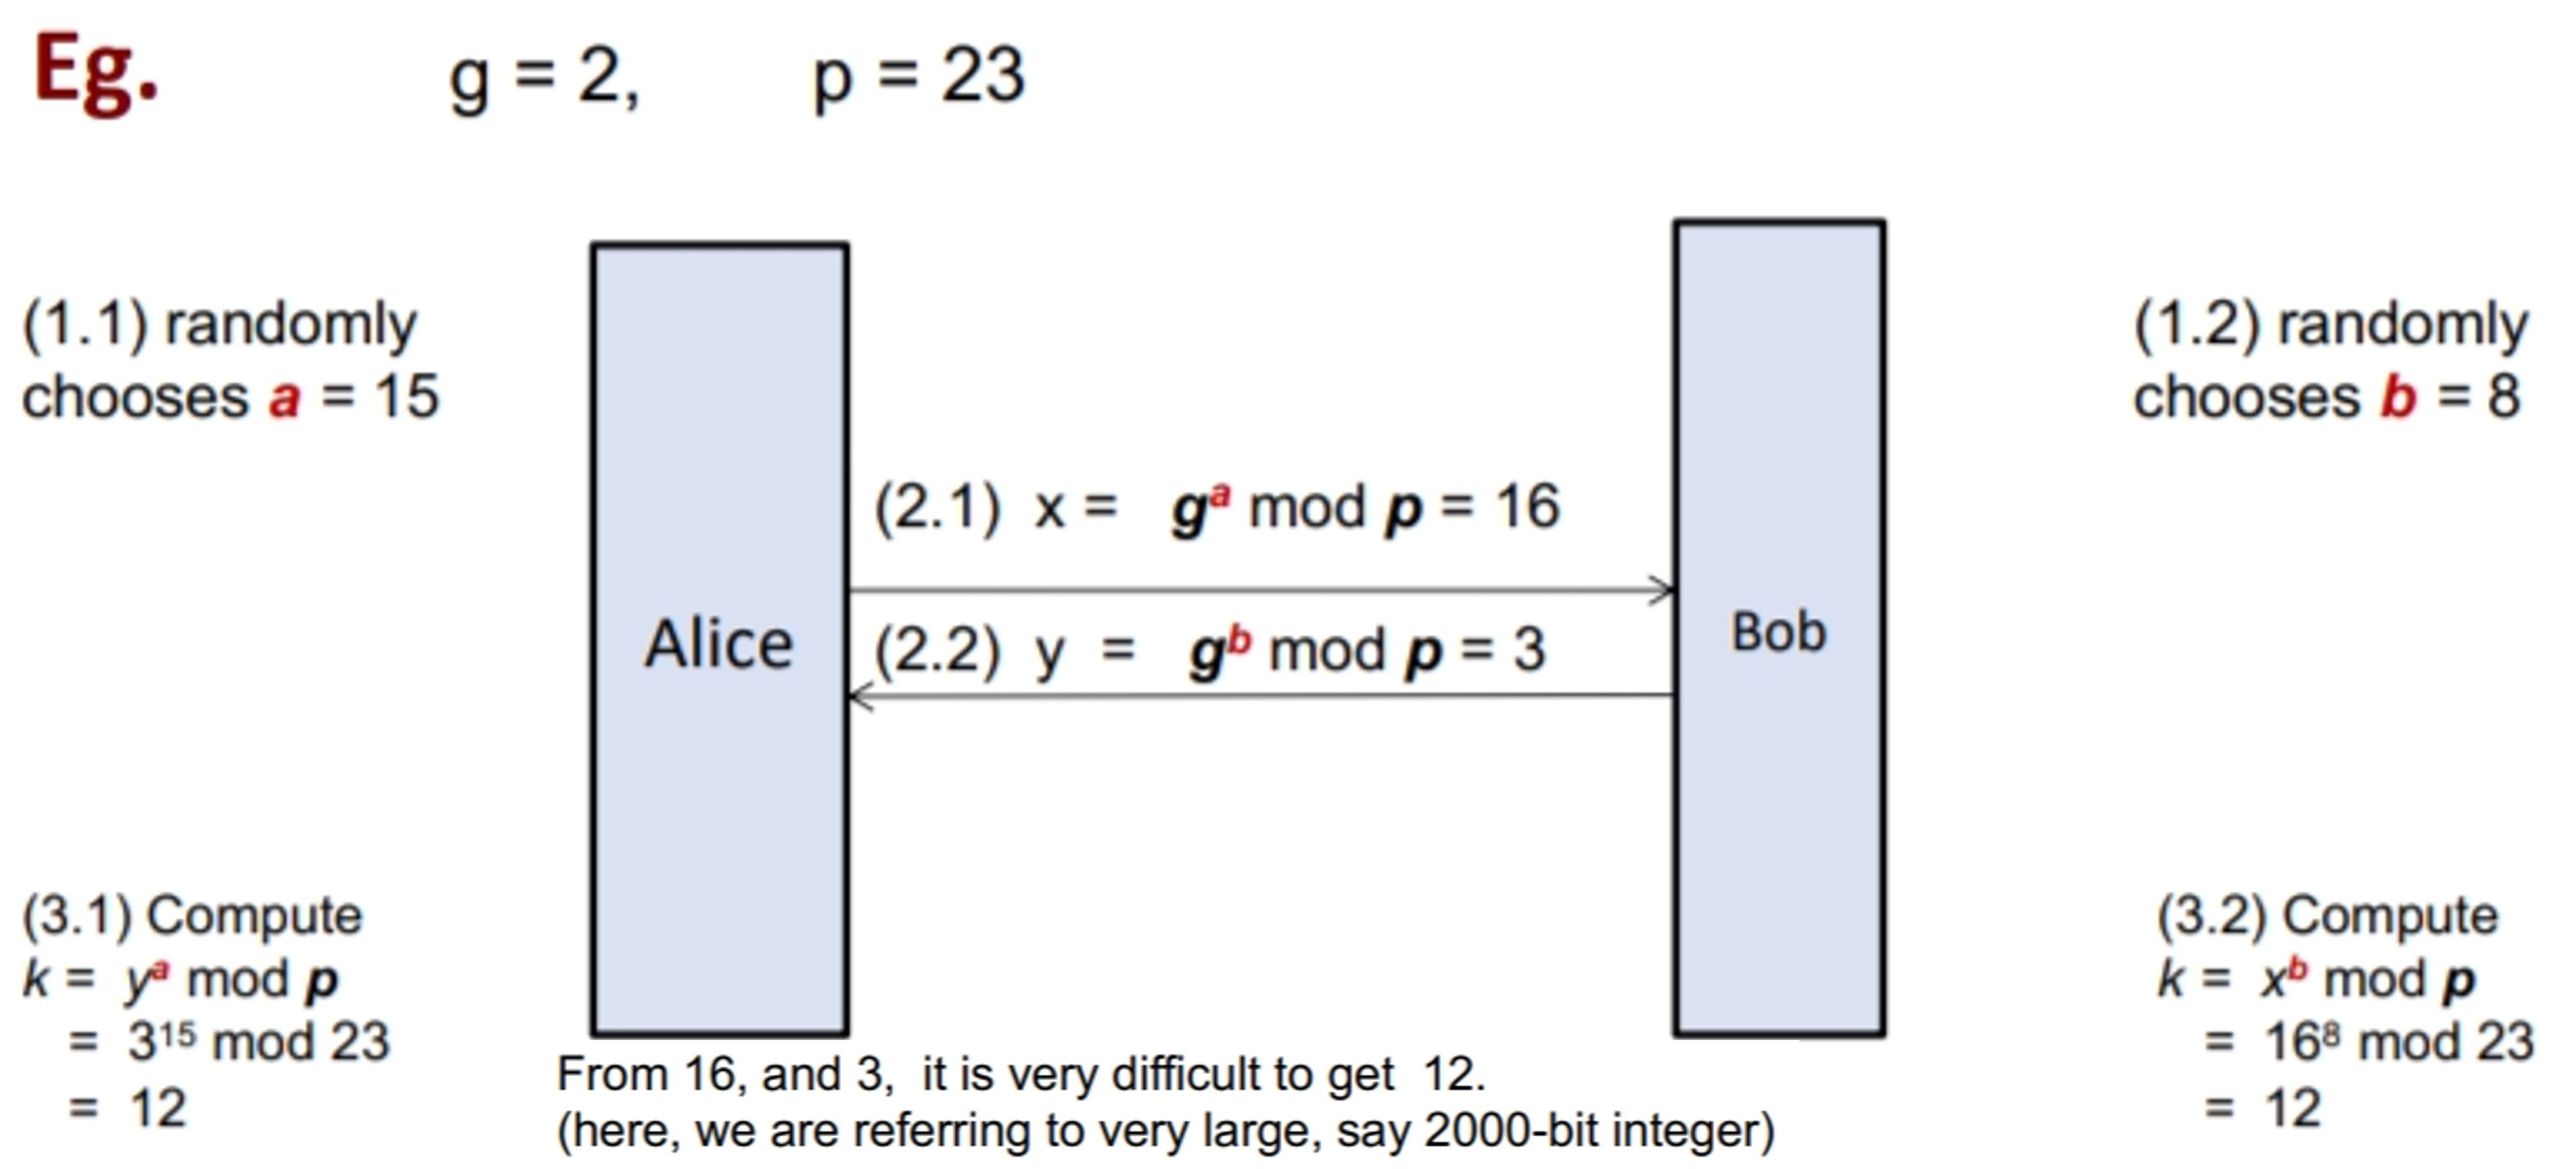
\includegraphics[width=1\linewidth]{DHKeyExchangeExample}}	

\null \null 
\null \null \null 
\columnbreak

\section{4.6 Authenticated Key-exchange Protocol}
Consider \textbf{malicious Mallory}, who can sniff, spoof and modify message.
\begin{itemize}
\item Mallory first allows Alice and Bob carry out strong authentication. After, Mallory interrupts and takes over channel. Mallory pretends to be
Bob! Even if employ challenge-response, Mallory still succeeds.
\end{itemize}
\centerline{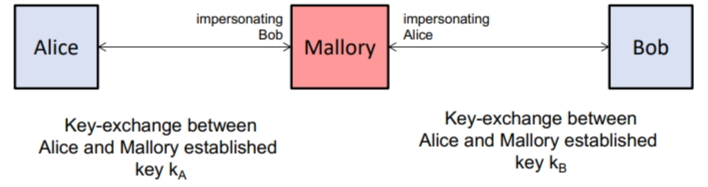
\includegraphics[width=0.7\linewidth]{authKeyExchangeMallory}}	

\begin{itemize}
\item \textbf{Authenticated Key-Exchange}: Protect subsequent interactions. \\
1. Authenticated key-exchange, outcome new shared secret session key $k$. \\
2. All subsequent communication protected (encrypted + mac) using $k$.
\end{itemize}
\centerline{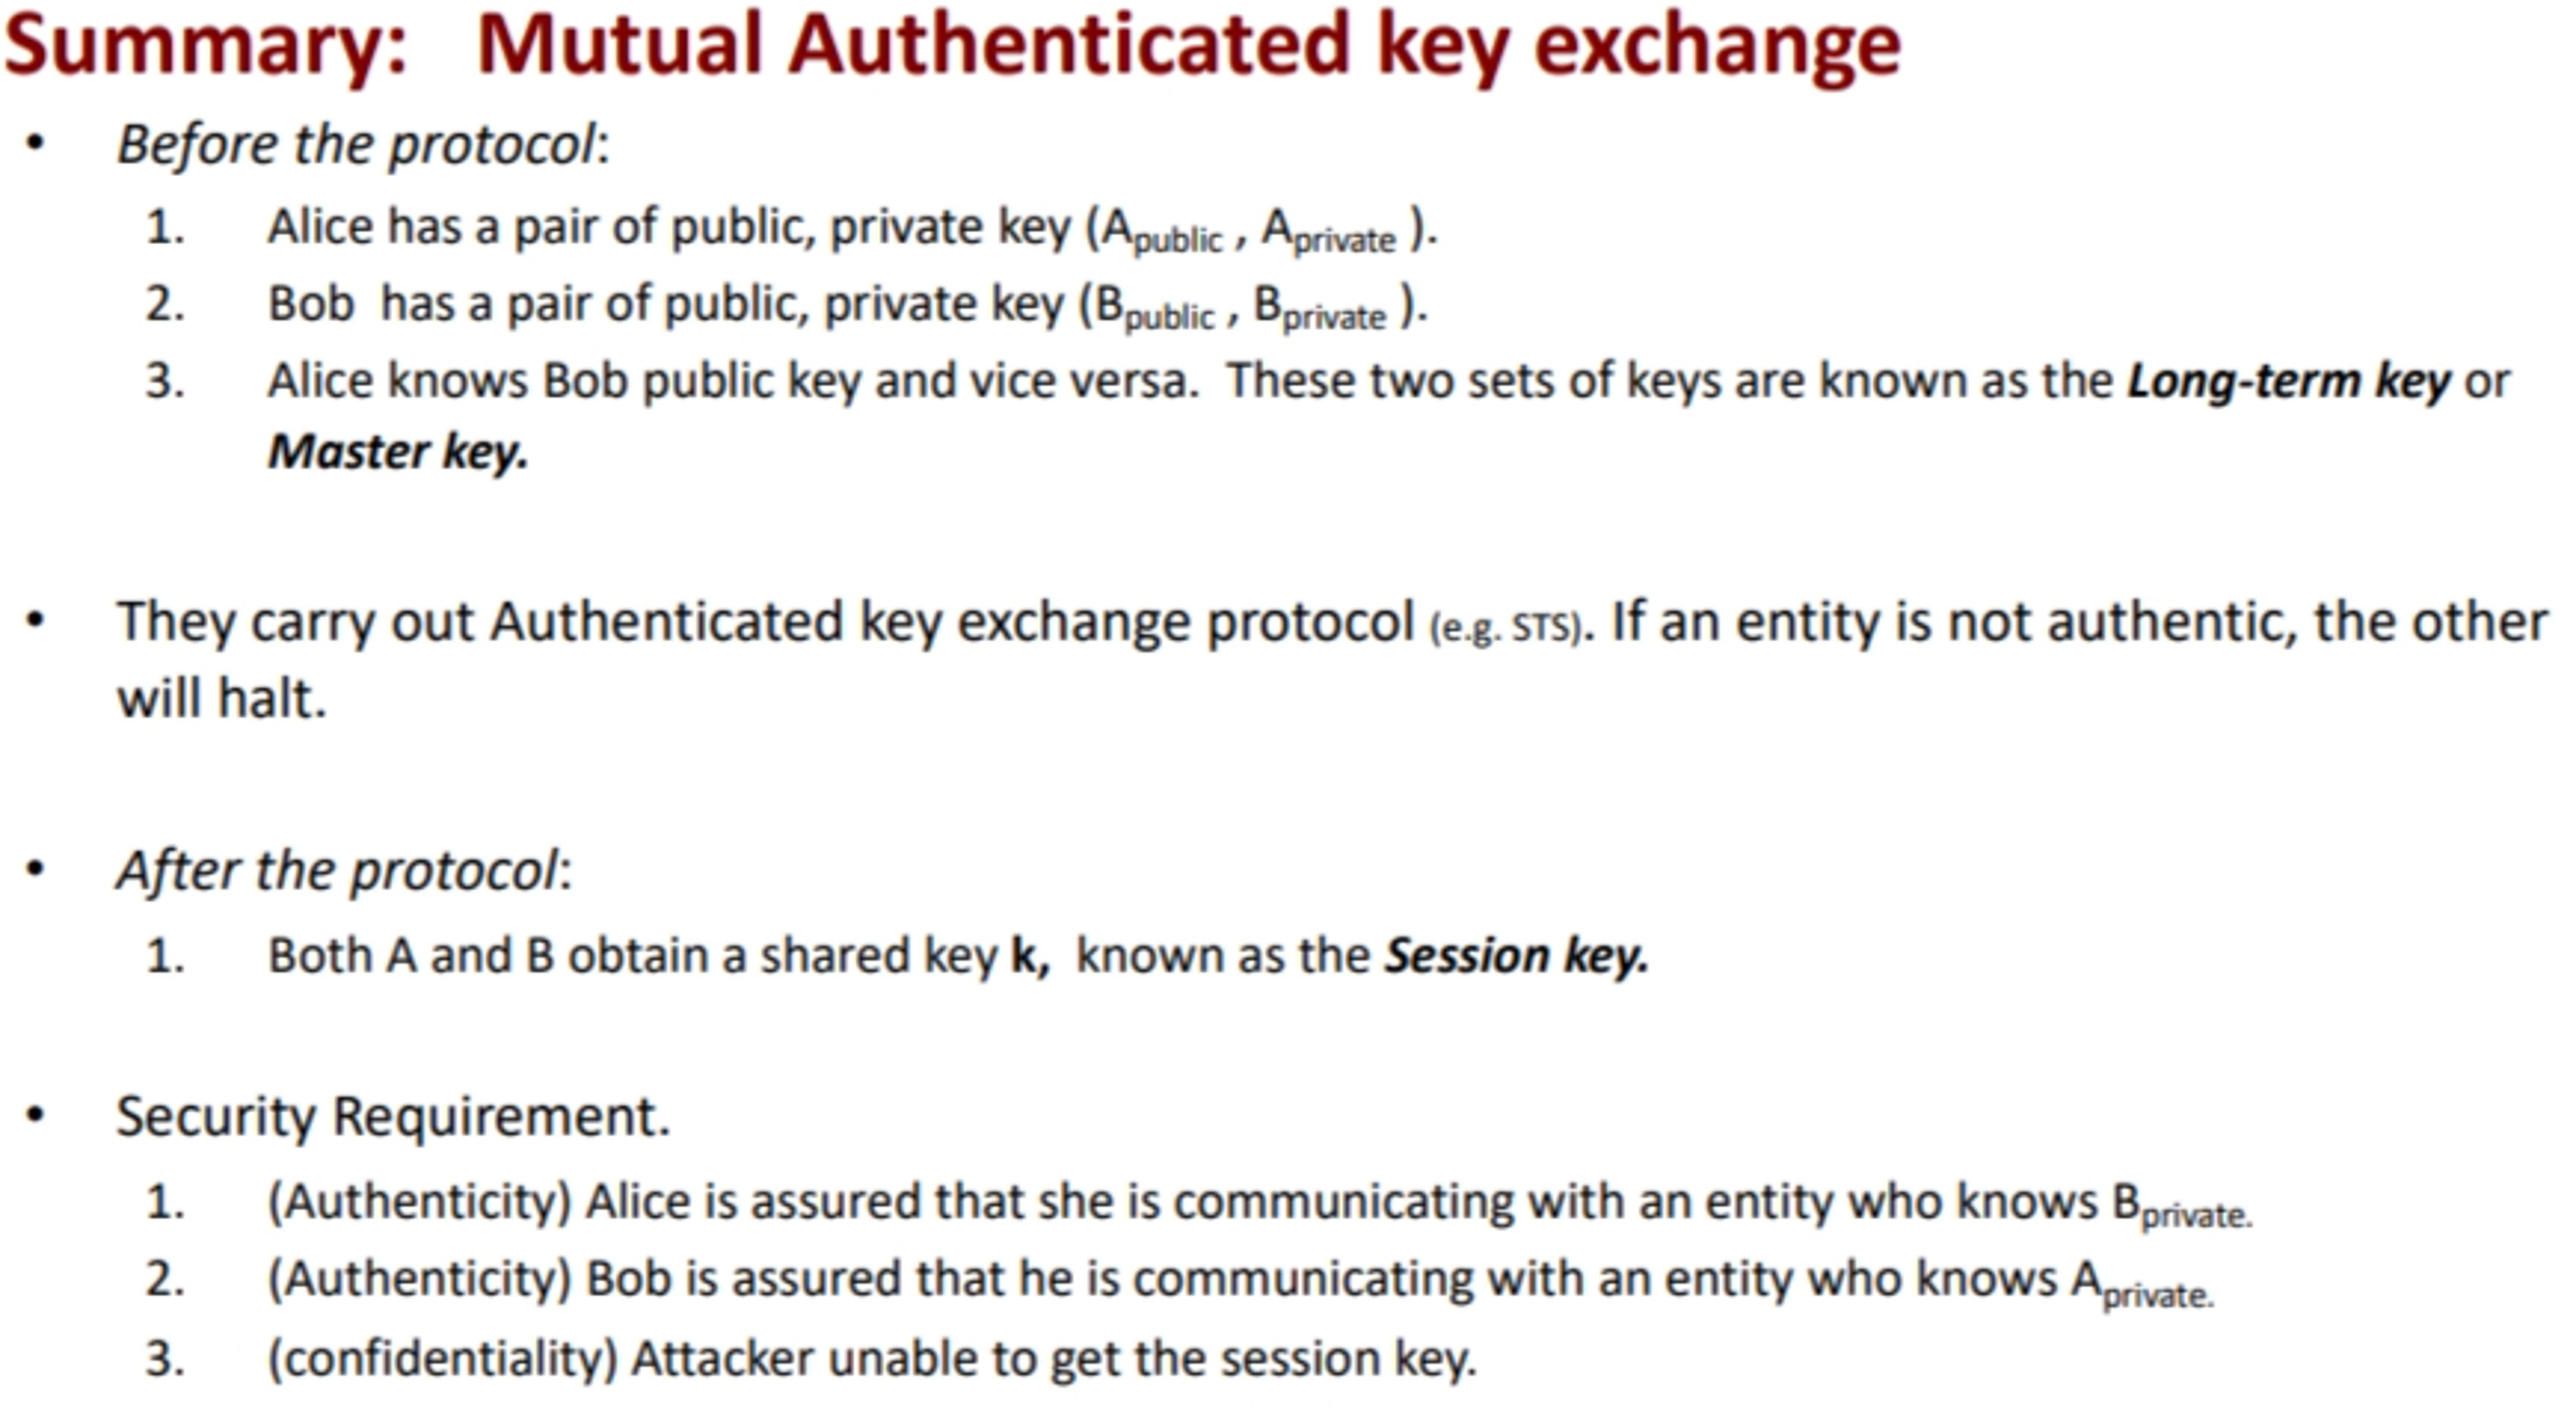
\includegraphics[width=1\linewidth]{authKeyExchangeSummary}}	

\begin{itemize}
\item Turns out authenticated key-exchange easily obtained from existing key-exchange, (either PKC-based key-exchange or DH-based key-exchange). Done by signing all
communication using the private key.
\item Special name for authenticated key-exchange that uses DH: it is known as \textbf{Station-To-Station Protocol (STS)}.
\end{itemize}

\subsection{Station-to-Station Protocol (based on DH)}
Assume both Alice and Bob agreed on two public parameters, generator $g$ and large (e.g. 1000 bits) prime $p$. Both g and p are not secret and known to the public.
Consider unilateral authentication. Alice want to authenticate Bob. Can be easily extended to mutual authentication. 
\centerline{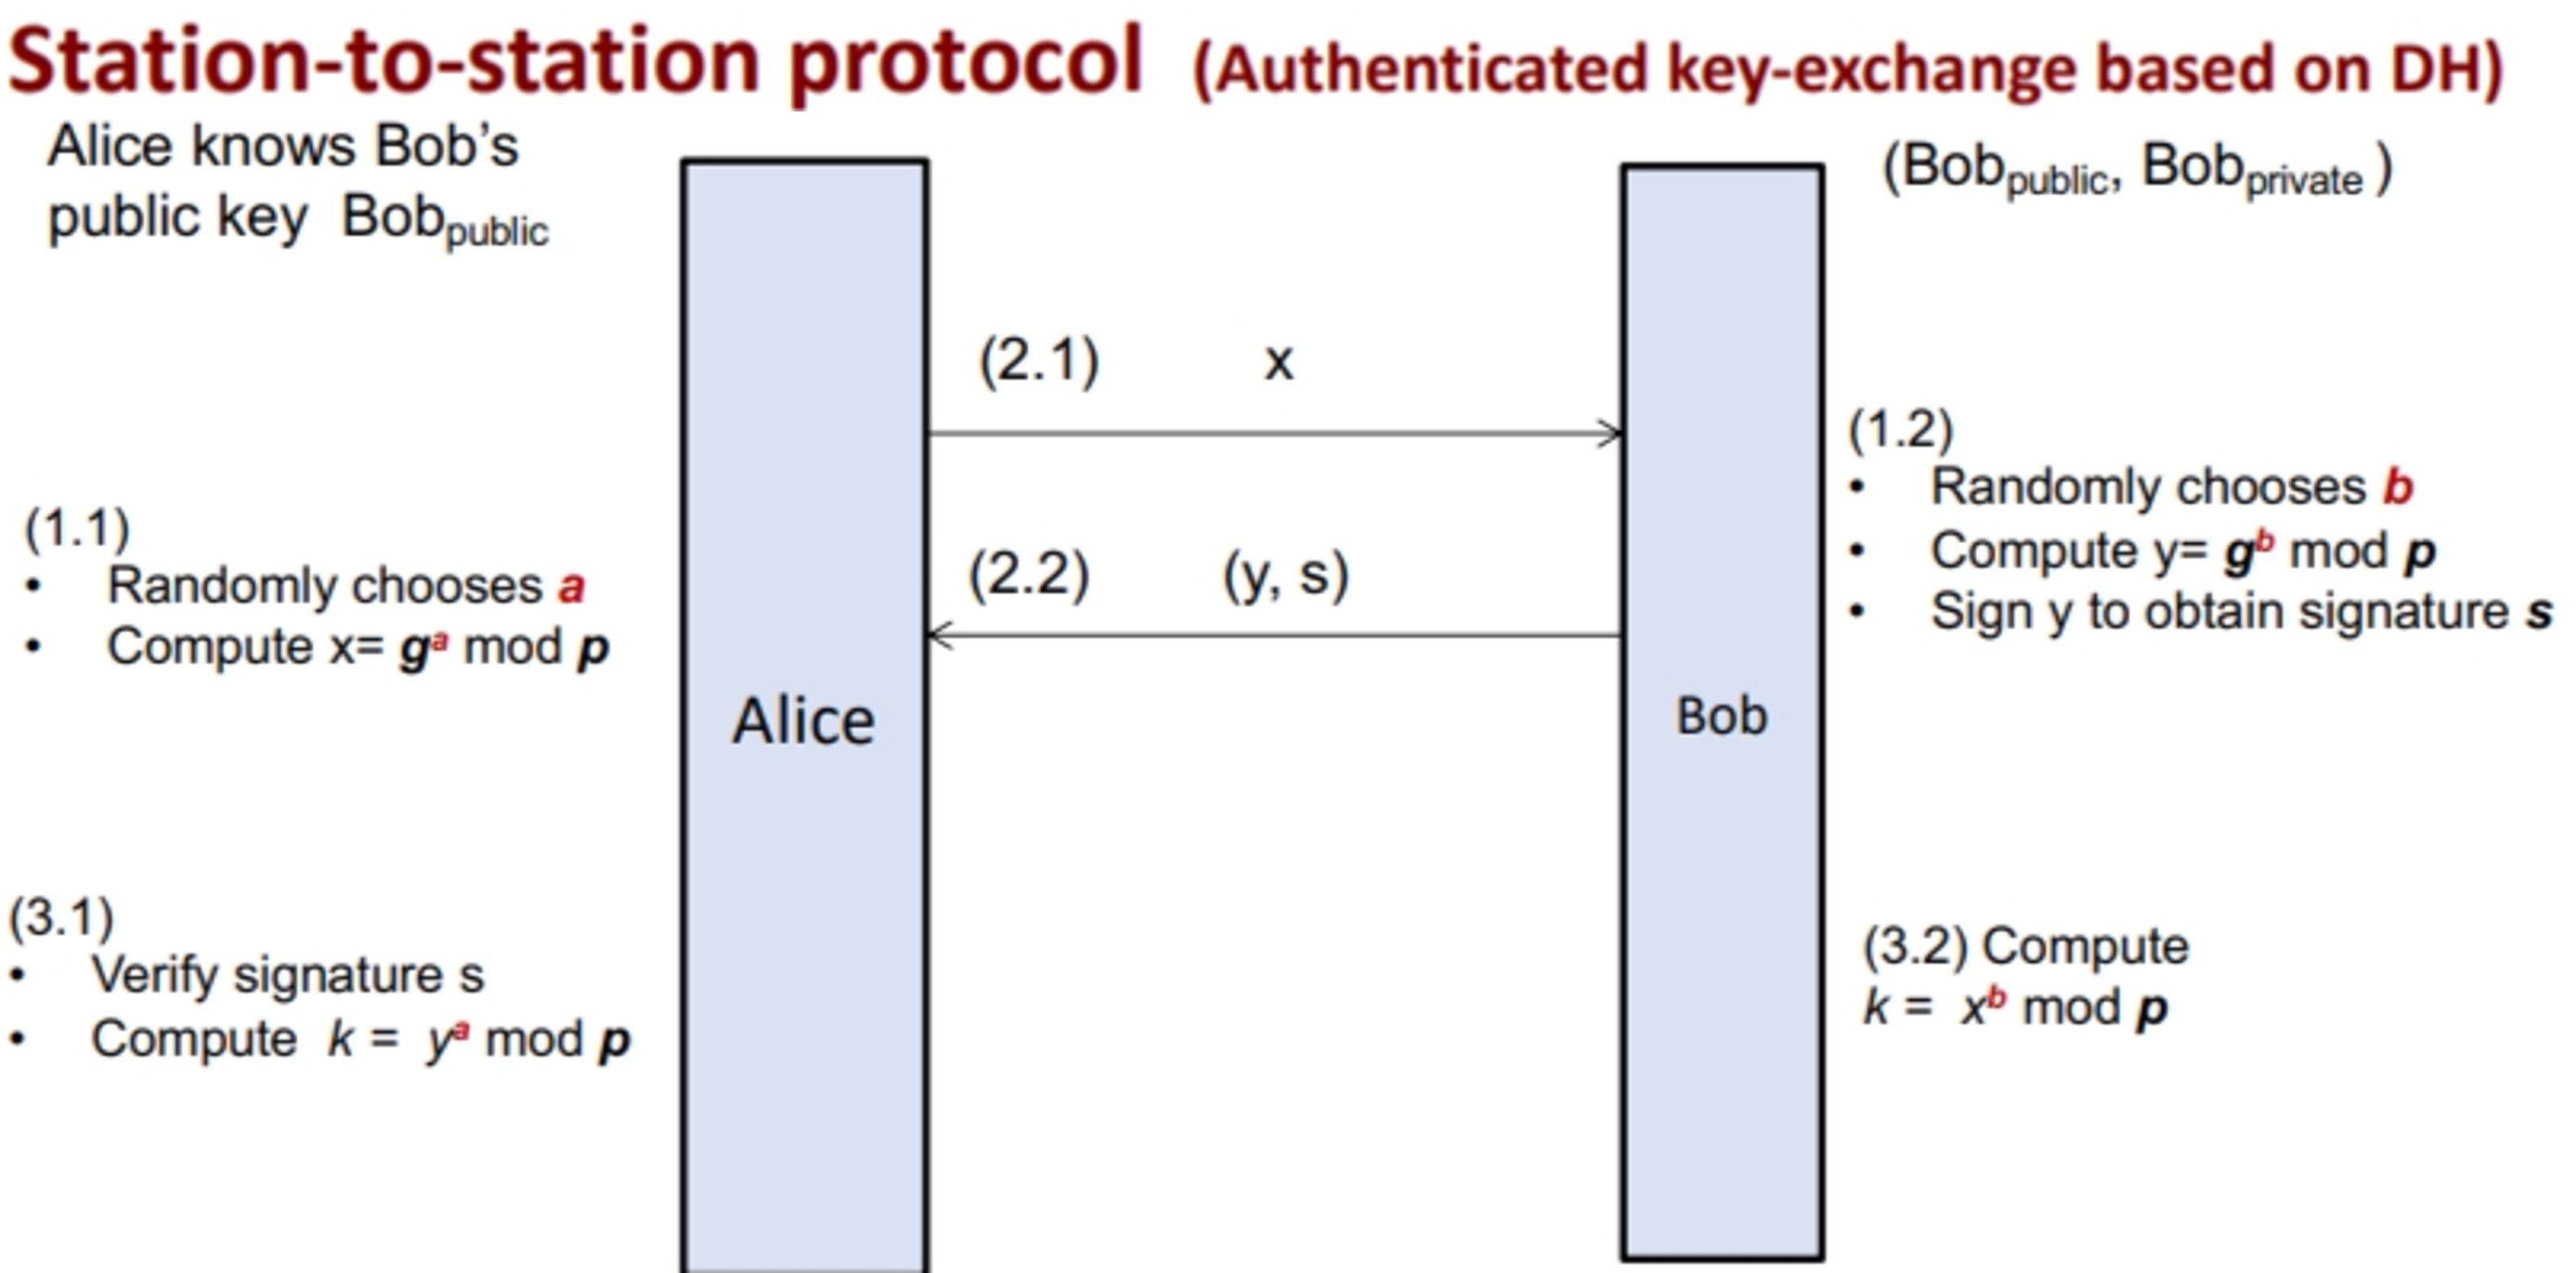
\includegraphics[width=1\linewidth]{stationToStation}}	
Remark: This is unilateral authentication. Can extend it to mutual by making Alice signs her messages in step (2.1).

\subsection{Password based Encrypted Key Exchange}
(Asymmetric) Previous authenticated key-exchange protocols such as Station-to-station are based on public key. 
\begin{itemize}
\item (Symmetric) There are also symmetric key version, i.e both entities share a symmetric key. An entity is authentic if it can prove to the other that it knows the key.
\item (Password) A special case of symmetric key is when the key is a password.
\item Password usually has very low entropy, thus potentially vulnerable to “offline” dictionary attack (see tutorial). There are secure protocols that, 
even if entropy of password low, still secure against offline dictionary attack (to guess password correct, attacker forced to interact with online server). These are called \textbf{“Password-Authenticated Key agreement” (PAKE).}
\end{itemize}

\centerline{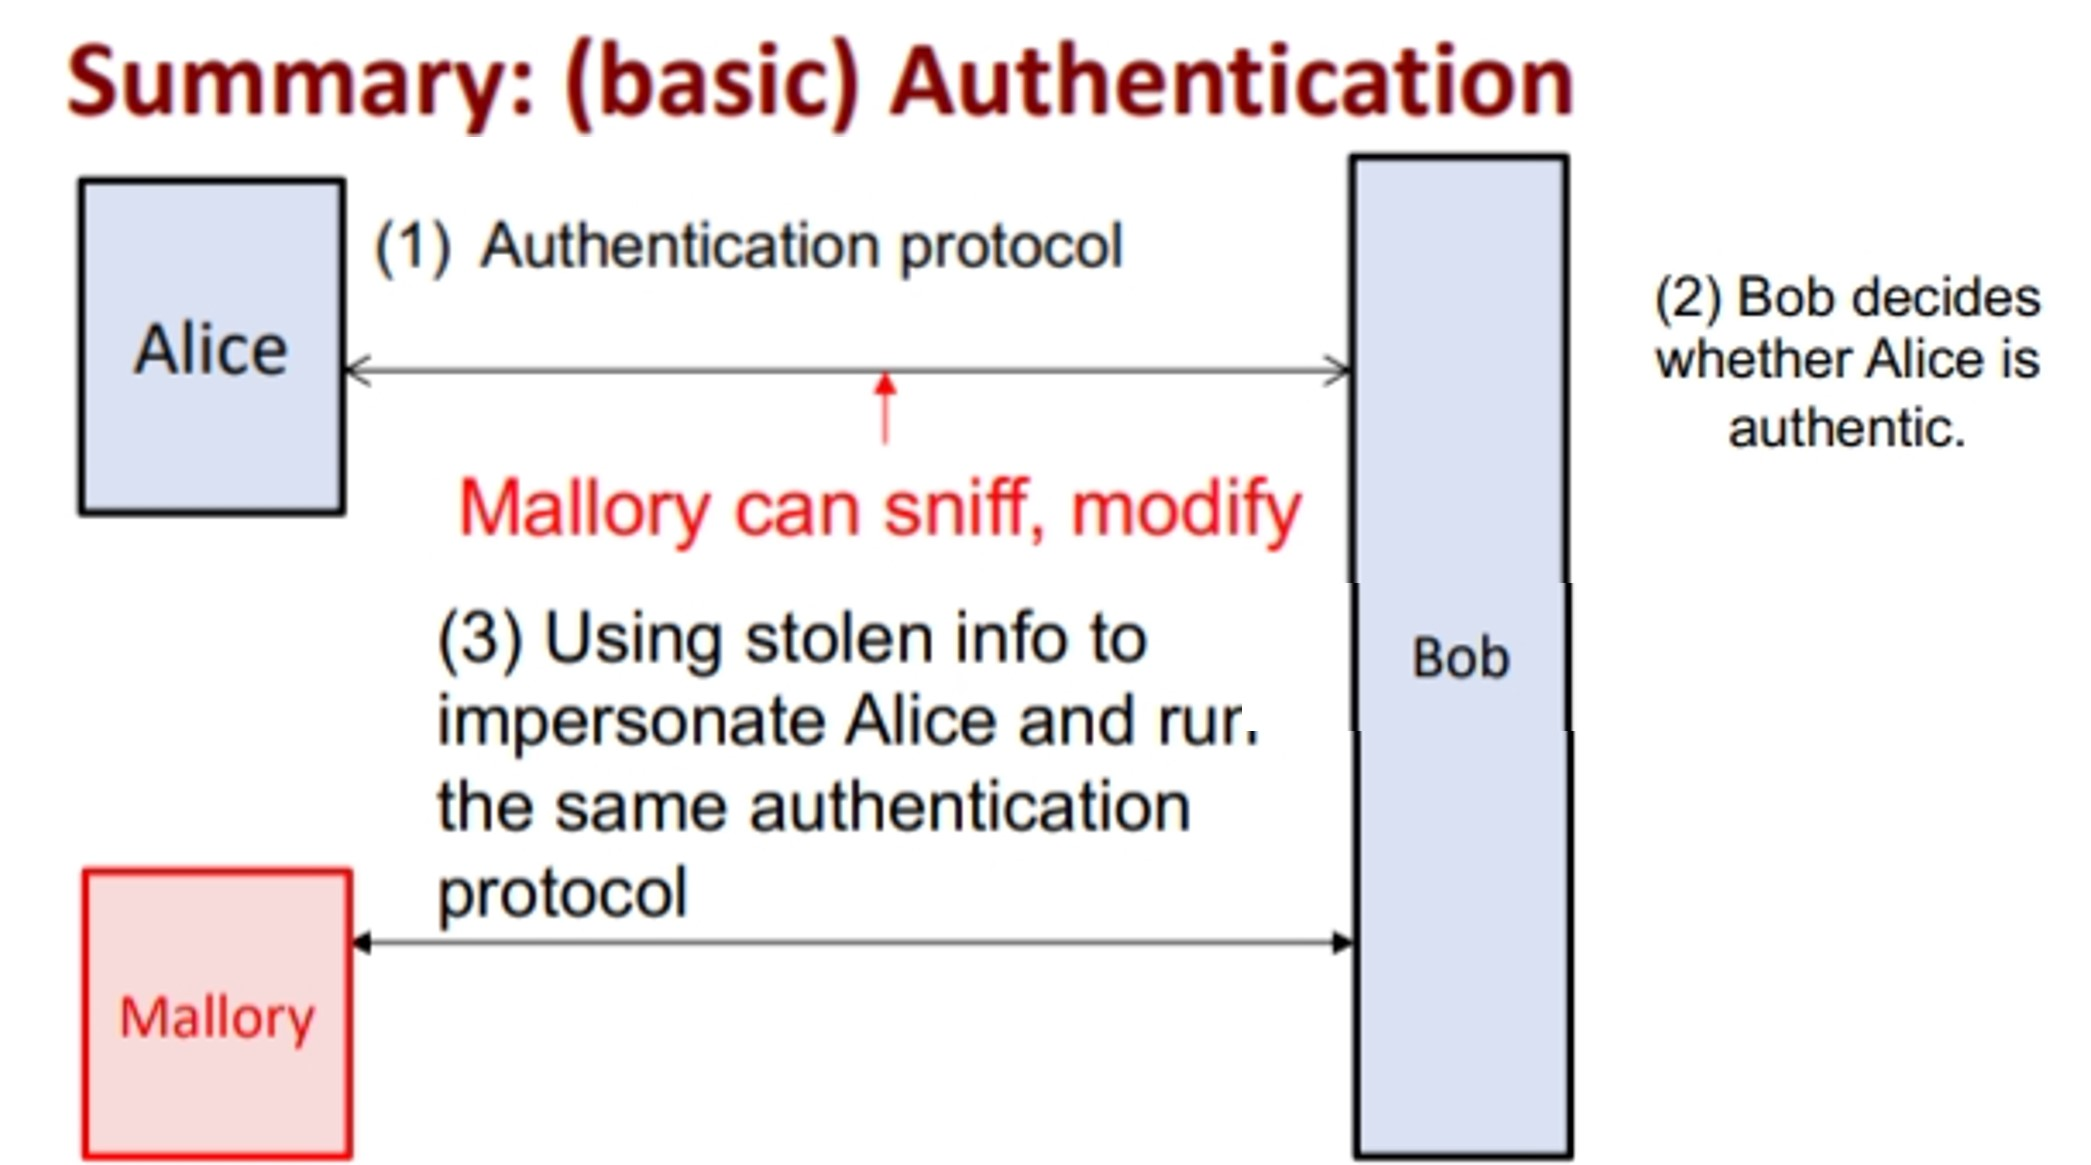
\includegraphics[width=0.8\linewidth]{authSummary4}}	
\medskip
\centerline{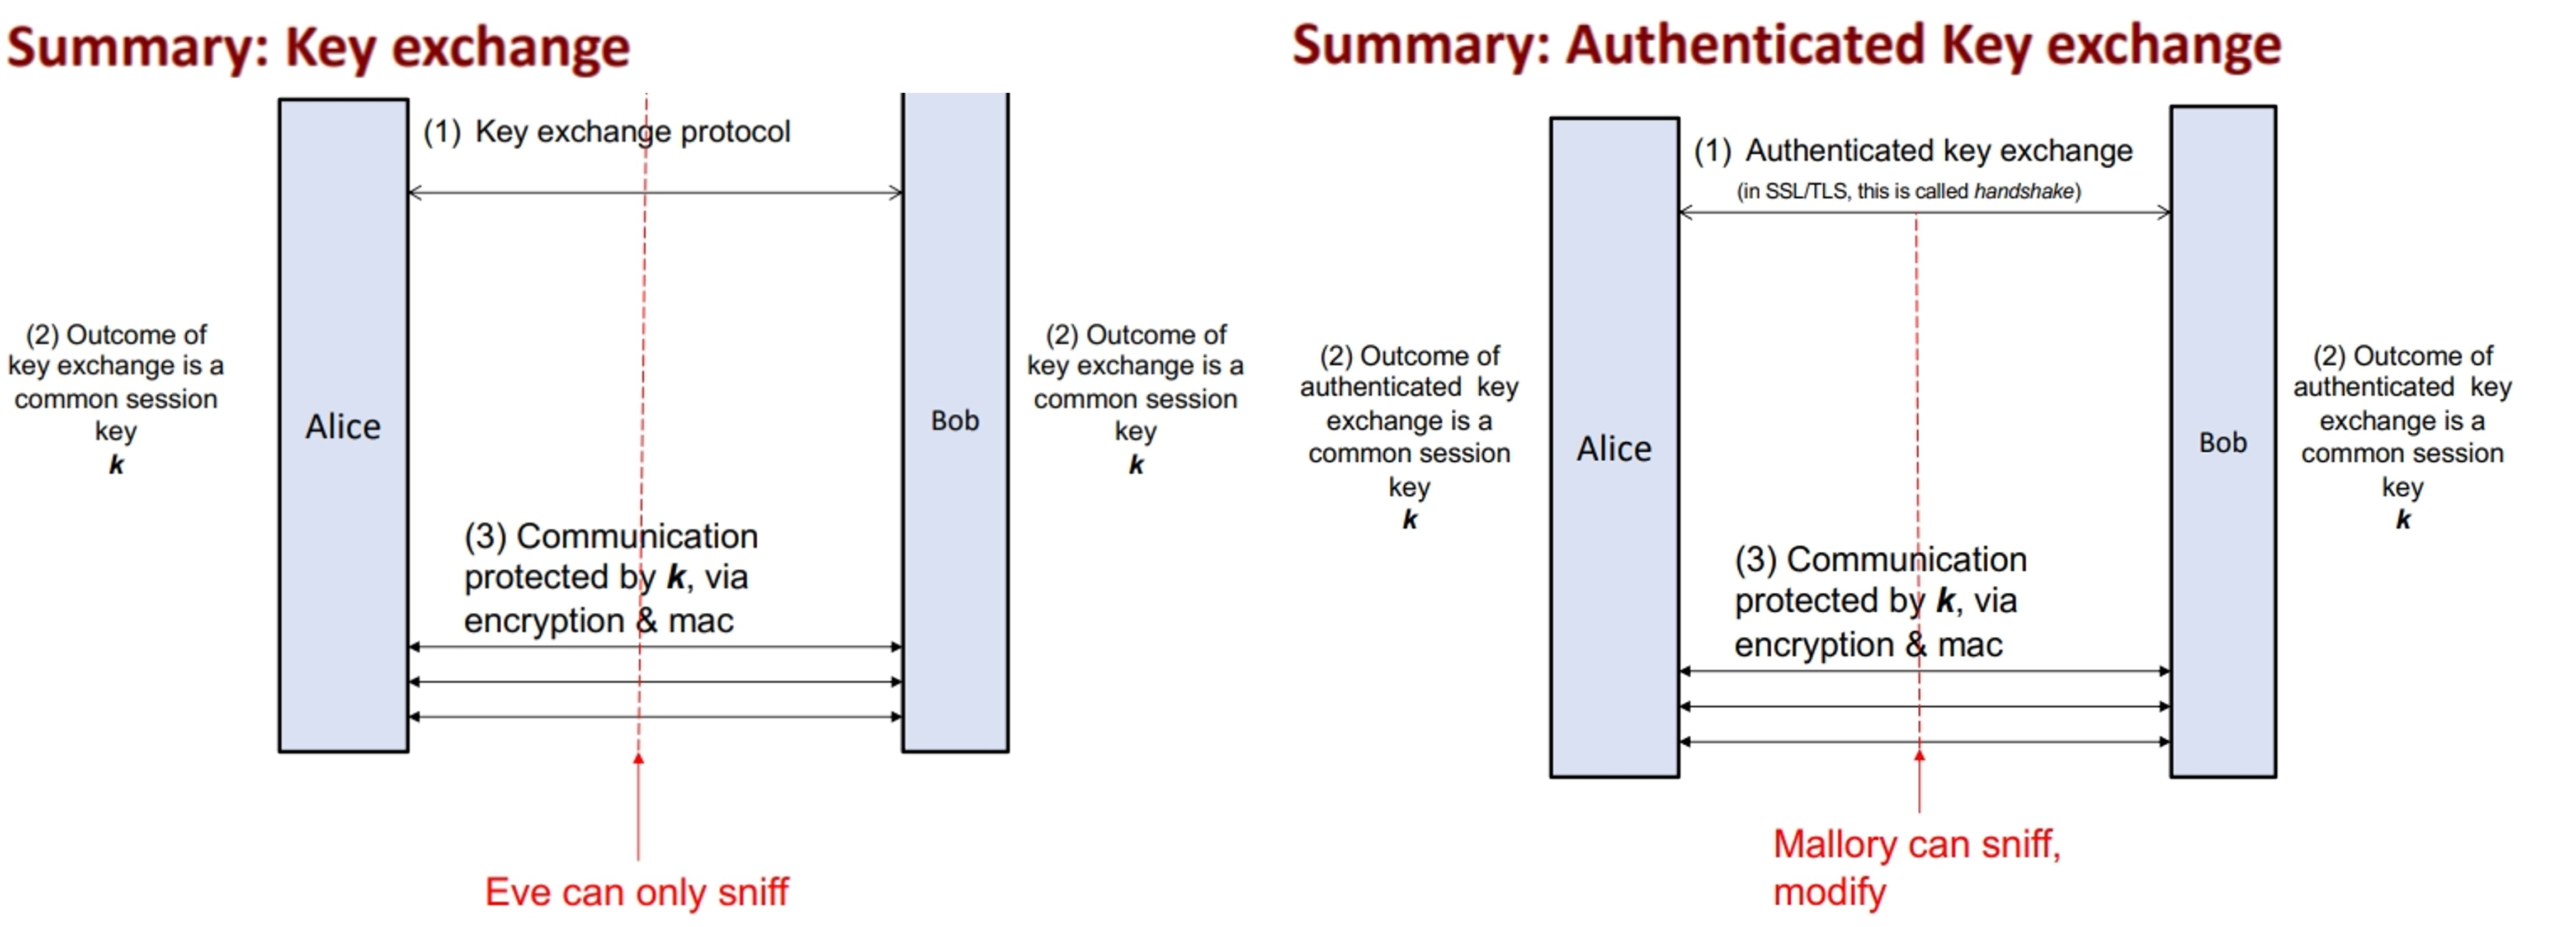
\includegraphics[width=1\linewidth]{authSummary5}}	




\section{4.7 Securing Communication Channel (Ensuring Channel Security)}
Given a "public channel" that facilitates communication, but presences of Mallory. Use unsecure public communication as carrier, add layer of crypto primitives on the messages, so channel is as secure as a “private channel”.
\begin{itemize}
\item \textbf{Scenario}: Alice wants to visit website Bob.com. Alice ueses free wifi called Mallory.  Everyone can access, thus public channel. Secure public channel using crypto. 
\end{itemize}
\centerline{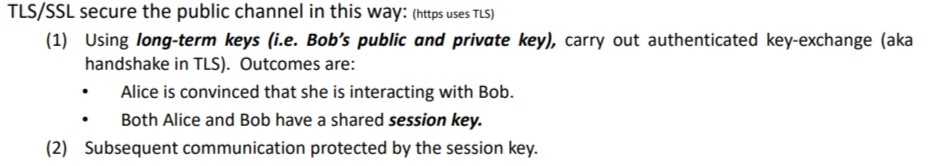
\includegraphics[width=1\linewidth]{tls1}}




\subsection{TLS: Transport Layer Security}
\centerline{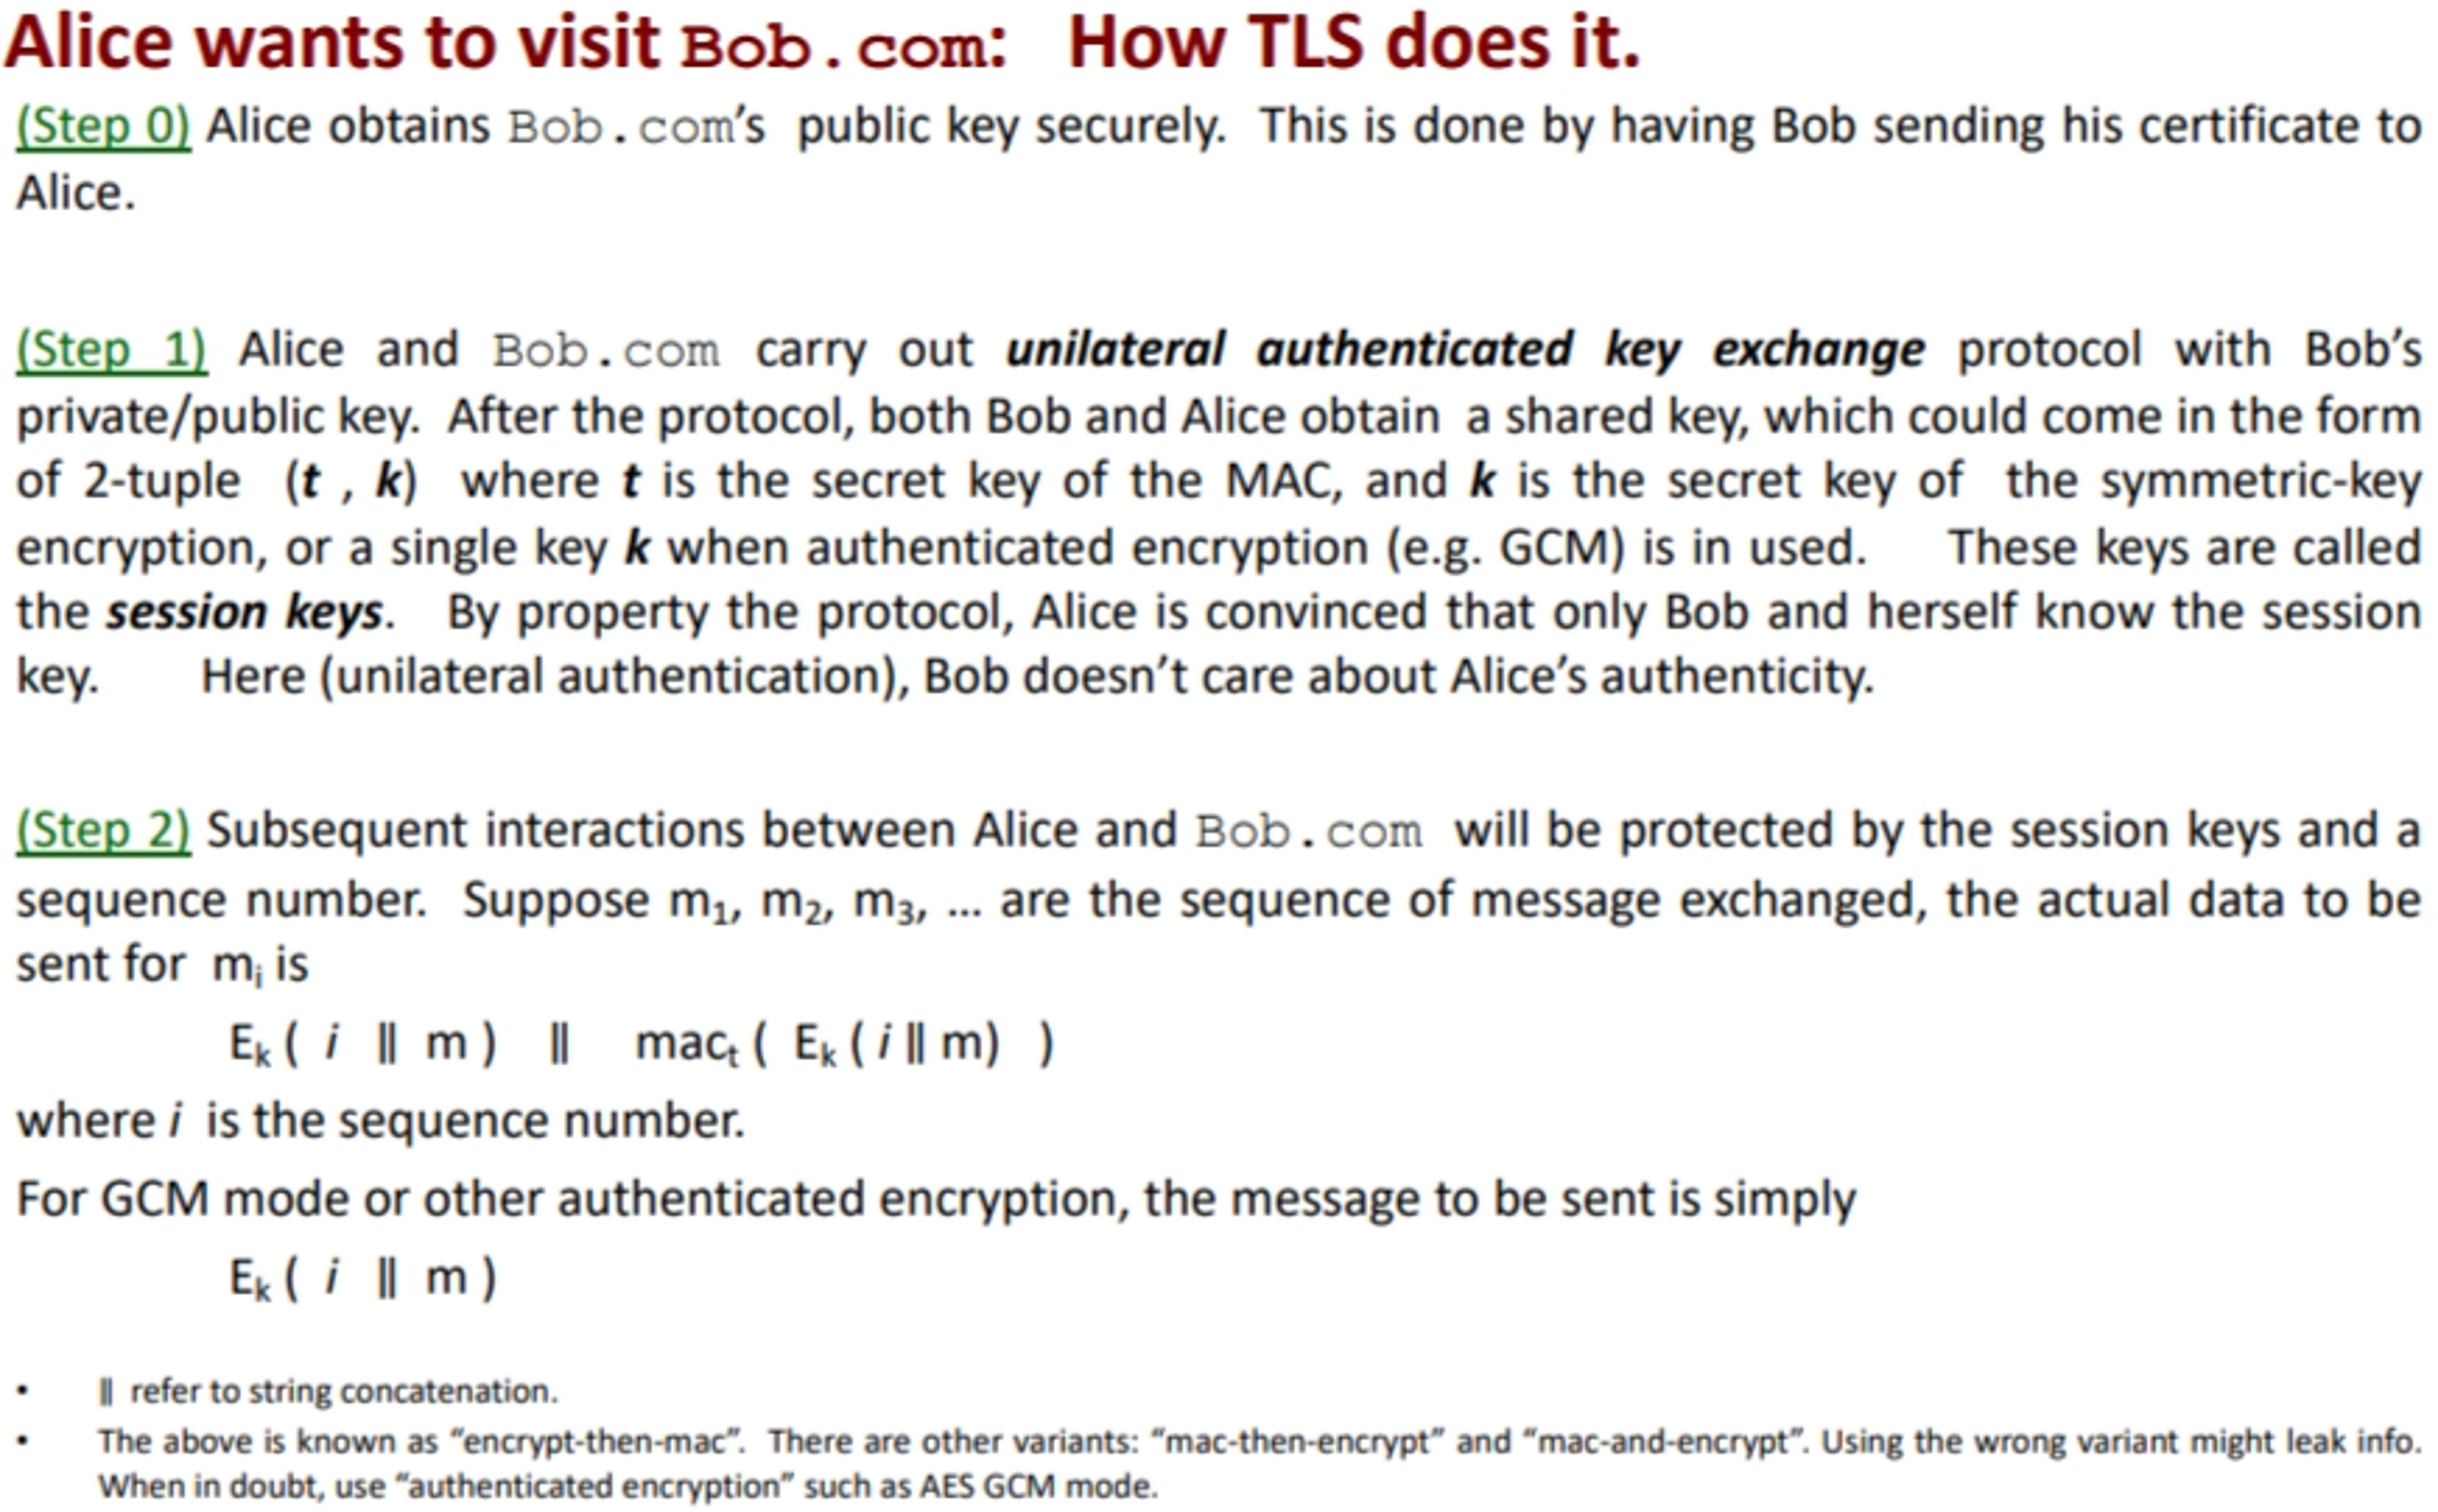
\includegraphics[width=1\linewidth]{tls2}}
\centerline{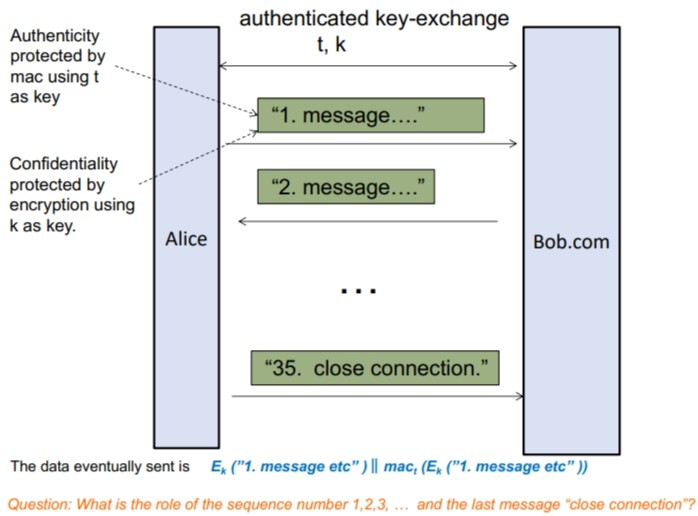
\includegraphics[width=1\linewidth]{tls3}}
Role of sequence number and last message is to make sure mallory is not able to add messages in between, or after the connection is closed.

\subsection{Relationship among TLS/SSL/https}
\begin{itemize}
\item SSL and Transport Layer Security (TLS) are protocols that secure communication using cryptographic mean. 
\item SSL is the predecessor of TLS. 
\item Https is built on top of TLS
\end{itemize}
\centerline{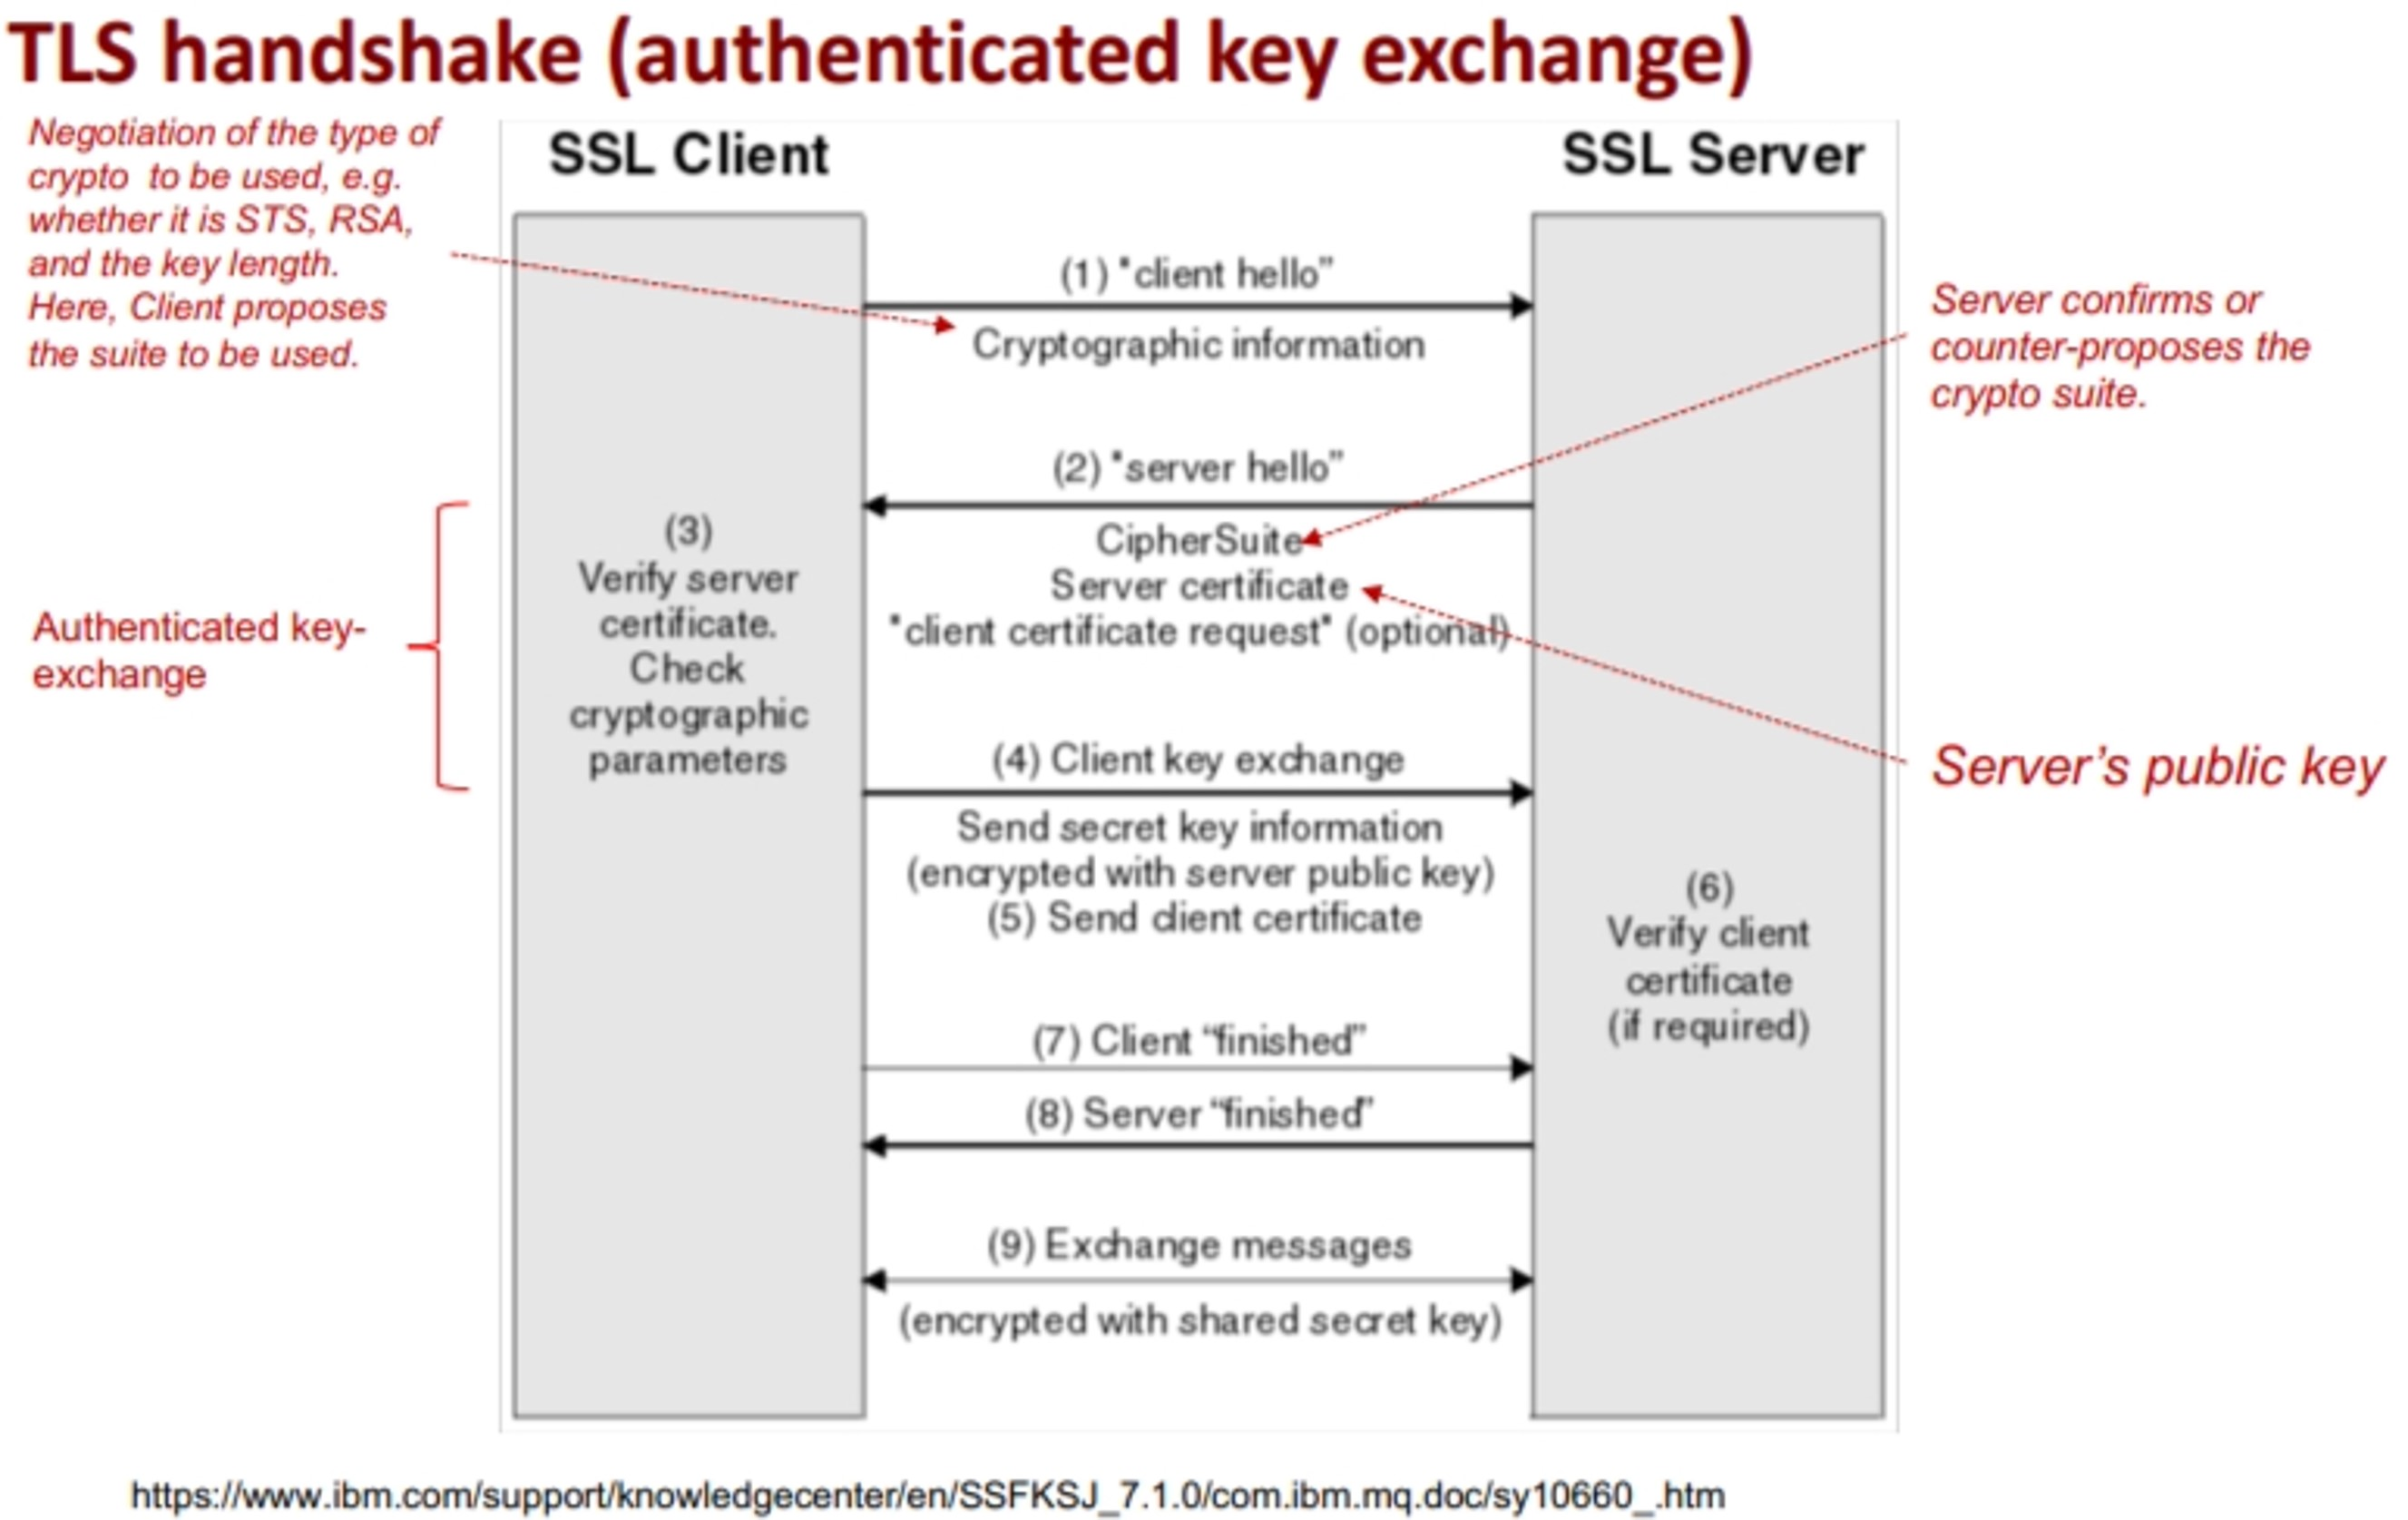
\includegraphics[width=0.9\linewidth]{tls4}}


\columnbreak 
\vfill\null
\columnbreak

\section{5. Network Security}
Cryptography and PKI establishes end-2-end security (w.r.t. Confidentiality \& authenticity) even in the presence of MITM. However, there are other issues in Networking, where Availability not addressed and Routing needs protection. We want to mitigate MITM as much as possible (e.g. concerned on implementation flaws, side-channel leakage, unprotected channels, etc).
\begin{itemize}
\item \textbf{Routing}: Layering. Intermediate nodes need to see and modify routing info at different “layers”. Protection at different layers. MITM in different layers
\item \textbf{Monitoring and segmentation}: Firewall, Intrusion Detection, DMZ, Server’s zone.
\item \textbf{Specific Attacks}: Name resolution attacks (poisoning, spoofing, ARP, DNS), Flaw in protocol (e.g. TLS renegotiation attack), Port Scanning, DDOS, botnets.
\item \textbf{Popular Protocols}: SSL/TLS (application), IPSEC (network), WPA (link)
\item What does padlock, https in browser mean? What can a MITM (in link layer) get? What can an attacker obtain via DNS spoofing?
\item Tools: Wireshark, nmap.
\end{itemize}

\section{5.1 Background on Networking}
\subsection{5.1.1 Brief Overview}
Computer Network establishes communication between large number of nodes. For robustness and resource sharing, use packet switching.
\begin{itemize}
\item \textbf{Network Security}: Attackers among intermediate nodes. Steal, modify (traffic routed to wrong places), disrupt. Guess who is talking to who.
\item \textbf{Multiple hops}: At each intermediate node, routing data read and modified.
\item \textbf{Network Layers}:  Partitions complex communication system into several abstraction layers. E.g. view layer-N protocol built upon a virtual connection at layer N-1. Passes down the message, level below abstracted.
\item \textbf{Ports}: Each node has total 65535 ports. If no process "listening" port to process data, port is "closed".
\item \textbf{Addressing Schemes (different Layers)}: A single node has different names in different layers.
\end{itemize}
\centerline{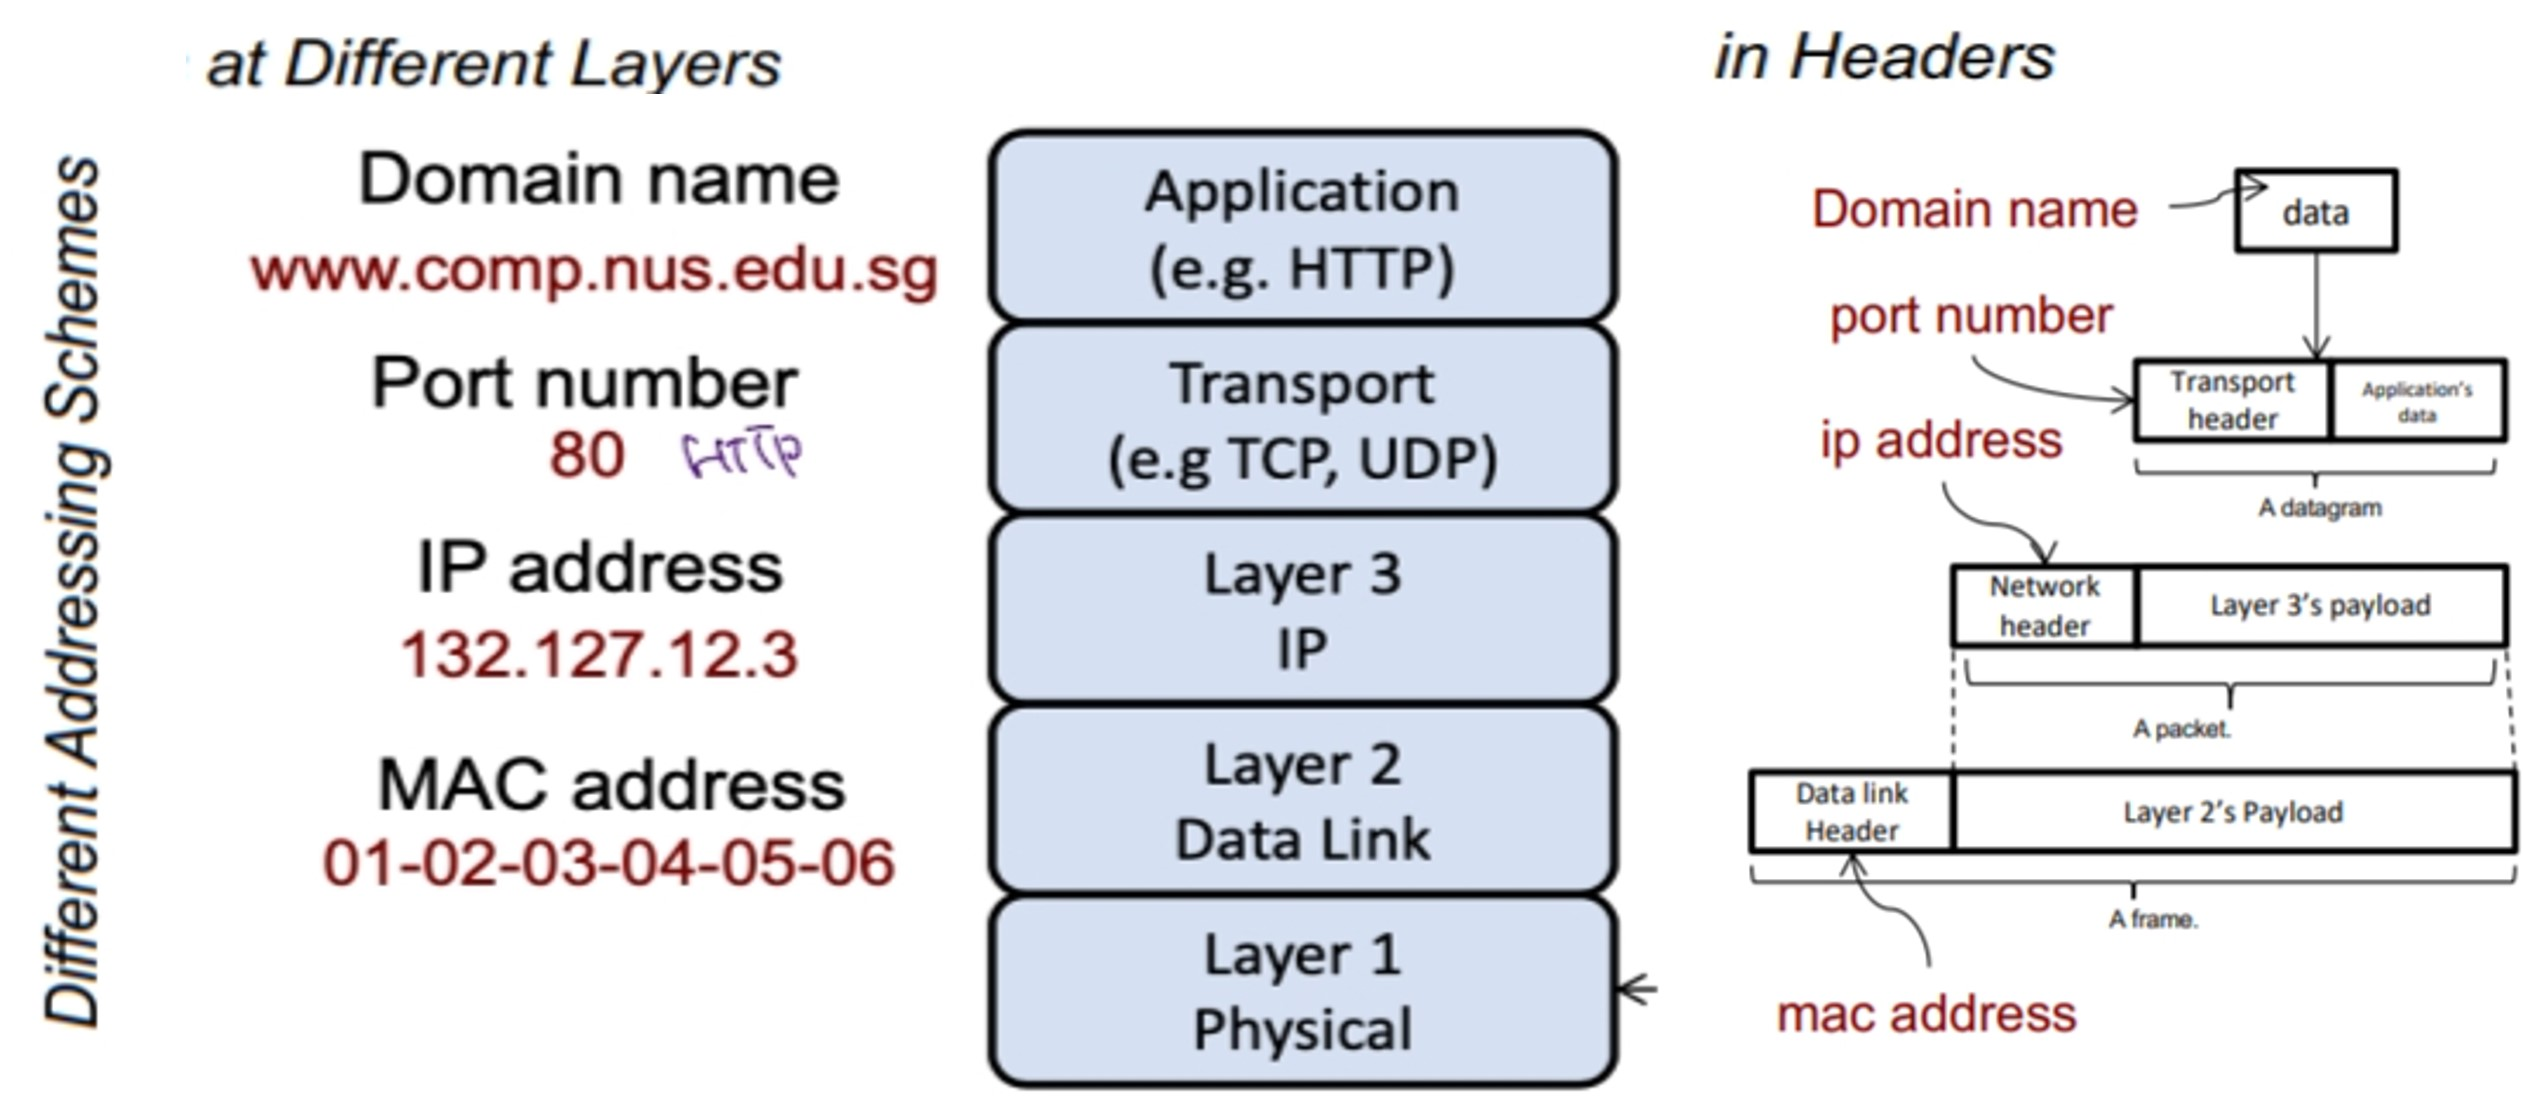
\includegraphics[width=0.9\linewidth]{addressingSchemes}}

\subsubsection{5.1.2 MITM: Man-In-The-Middle}
A MITM sits in-between two communicating parties. Unless otherwise stated, the MITM can sniff, spoof, modify, drop the data. 
Very often, when mentioning a MITM, it is clear from context which part of the header the MITM has access to.
\begin{itemize}
\item \textbf{MITM in Layer x}: we mean a MITM along the virtual connection in layer x. The MITM can see and modify data unit in that layer. For IP 
layer, the MITM has access to the IP packet, including the header and payload.
\item E.g. Evil cafe owner free wifi can MITM in Data Link layer, sniff, spoof, modify, drop. Anyone in cafe tapping in wirelessly is MITM in physical layer who can sniff, spoof, but not drop, nor modify. 
\end{itemize}


\section{5.2 Name Resolution and Attacks}
Each peer entity has a name. A single node may have different "name" at different layer. Initial design of resolution protocols did not take security into account, easy for attackers to manipulate outcome. 

\begin{itemize}
\item \textbf{Domain Name System (DNS)}: maps domain names to their respective IP addresses. It uses a hierarchical decentralized naming system. An attacker can thus target the association of the domain name with the IP address.
\item \textbf{Address Resolution Protocol (ARP)}: associates or maps IP addresses (logical addresses) with MAC addresses (physical addresses). Uses broadcast mechanism on a local network. An attacker on the local network can target the association.
\end{itemize}

\subsection{Domain Name System (DNS) Attack}
\textbf{Name Resolution}: Given a domain name (e.g. www.comp.nus.edu.sg), its IP address found by looking up locally stored host table, or querying DNS server.
\begin{itemize}
\item The entity (aka client) initiating query (UDP protocol) is resolver. If address found, domain name is resolved. 
\item Each query contains 16-bit number, Query ID (QID). Response from name server must contain QID. If QID in response no match query QID, client rejects answer. 
\item Note no encryption or MAC involved, QID was probably not meant for authentication, but as efficient way to match multiple queries. 
\item \textbf{DNS server resolves domain name}, can be the “single-point-of-failure” for network. 
\item A DoS attacks, instead of attacking a Web server, could attack the DNS server instead.
\end{itemize}

\centerline{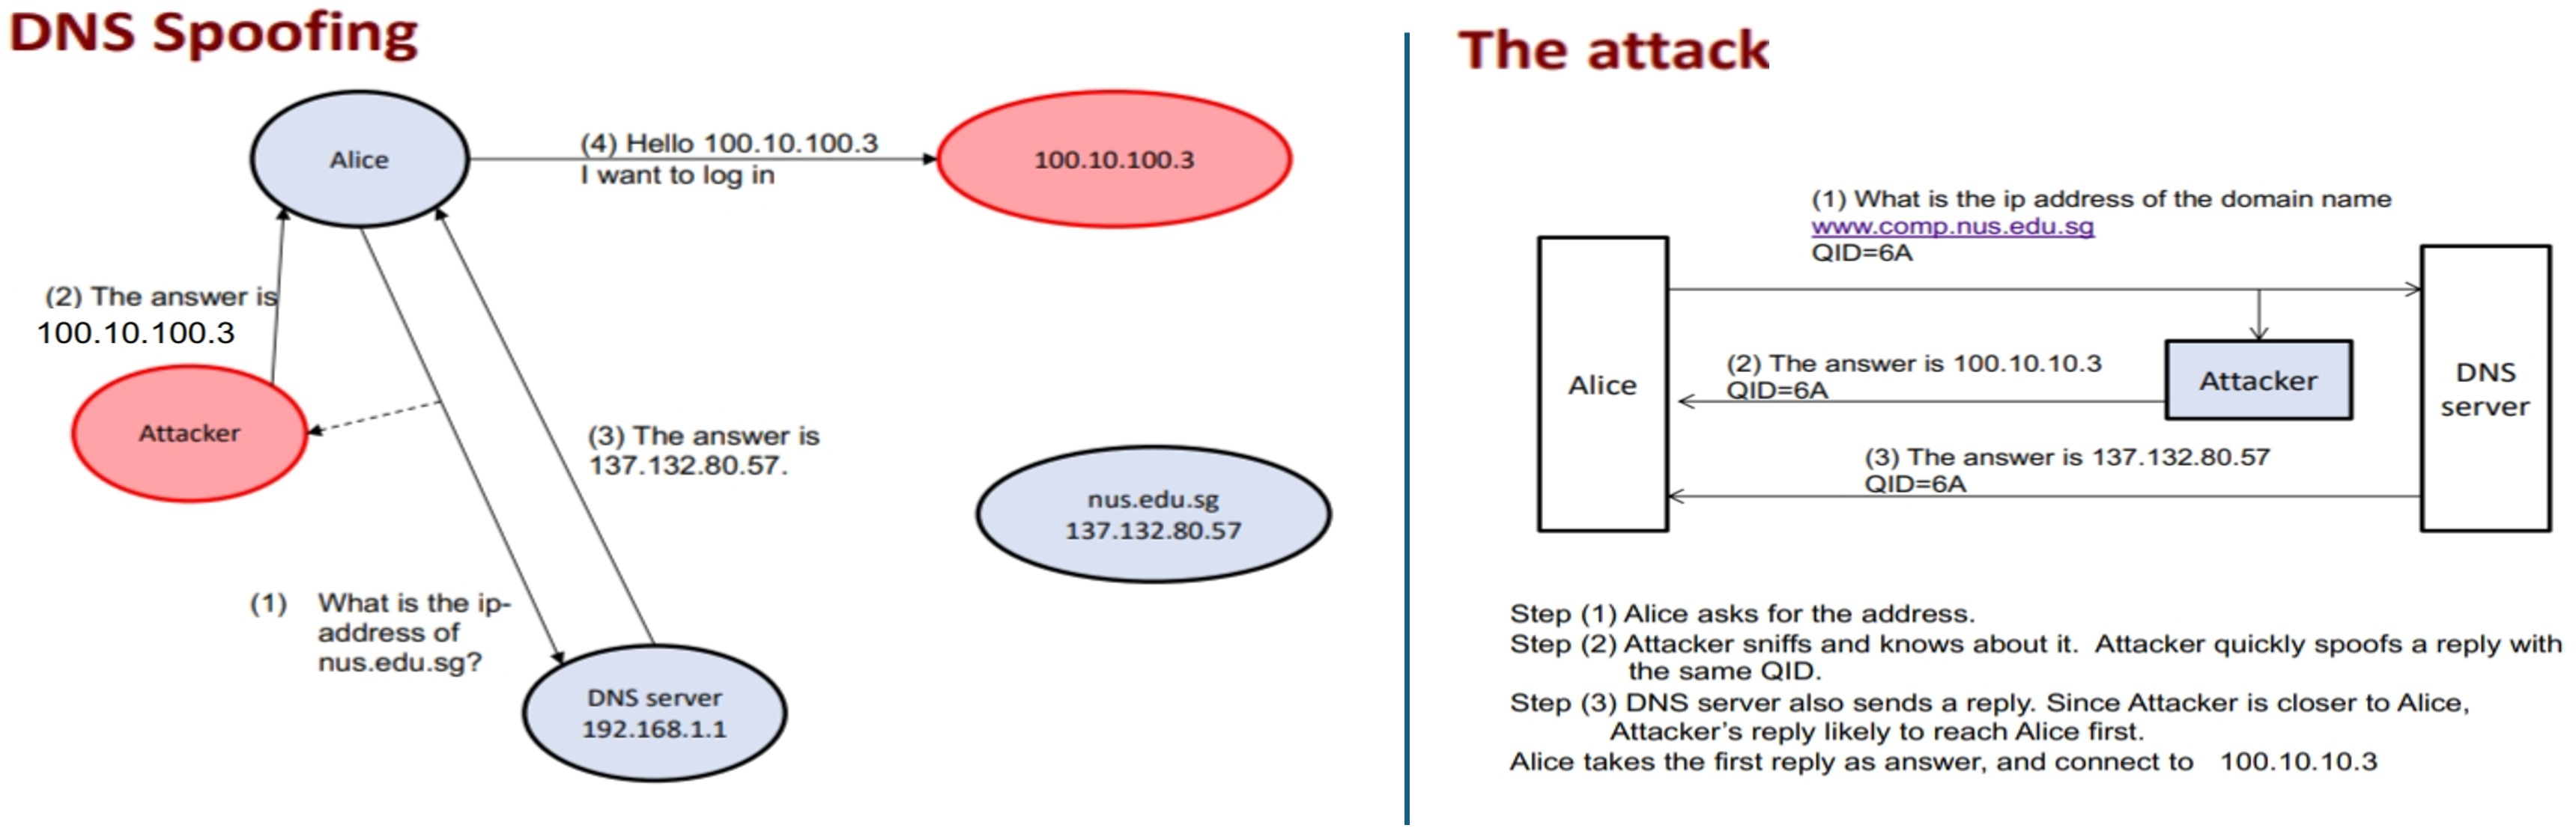
\includegraphics[width=1\linewidth]{DNSSpoofing}}

\subsection{Poisoning attack on ARP table}
A switch connects a few nodes. (Note that switch handles mac-addresses, router handles ip-addresses.) E.g. our home wifi “router”, although often called as a “router”, it also functions as a switch. It contains a gateway which performs routing.
\begin{itemize}
\item Switch connect ports based on mac-addresses, has ARP table associating port to mac-addresses.
\item Resolution of IP to MAC address done by nodes (e.g. phone) with own ARP table. Nodes update each others (ARP query mechanism).
\item \textbf{ARP poisoning} is an attack that modifies (aka “poisons”) the tables so as to gain MITM access.
\end{itemize}
\centerline{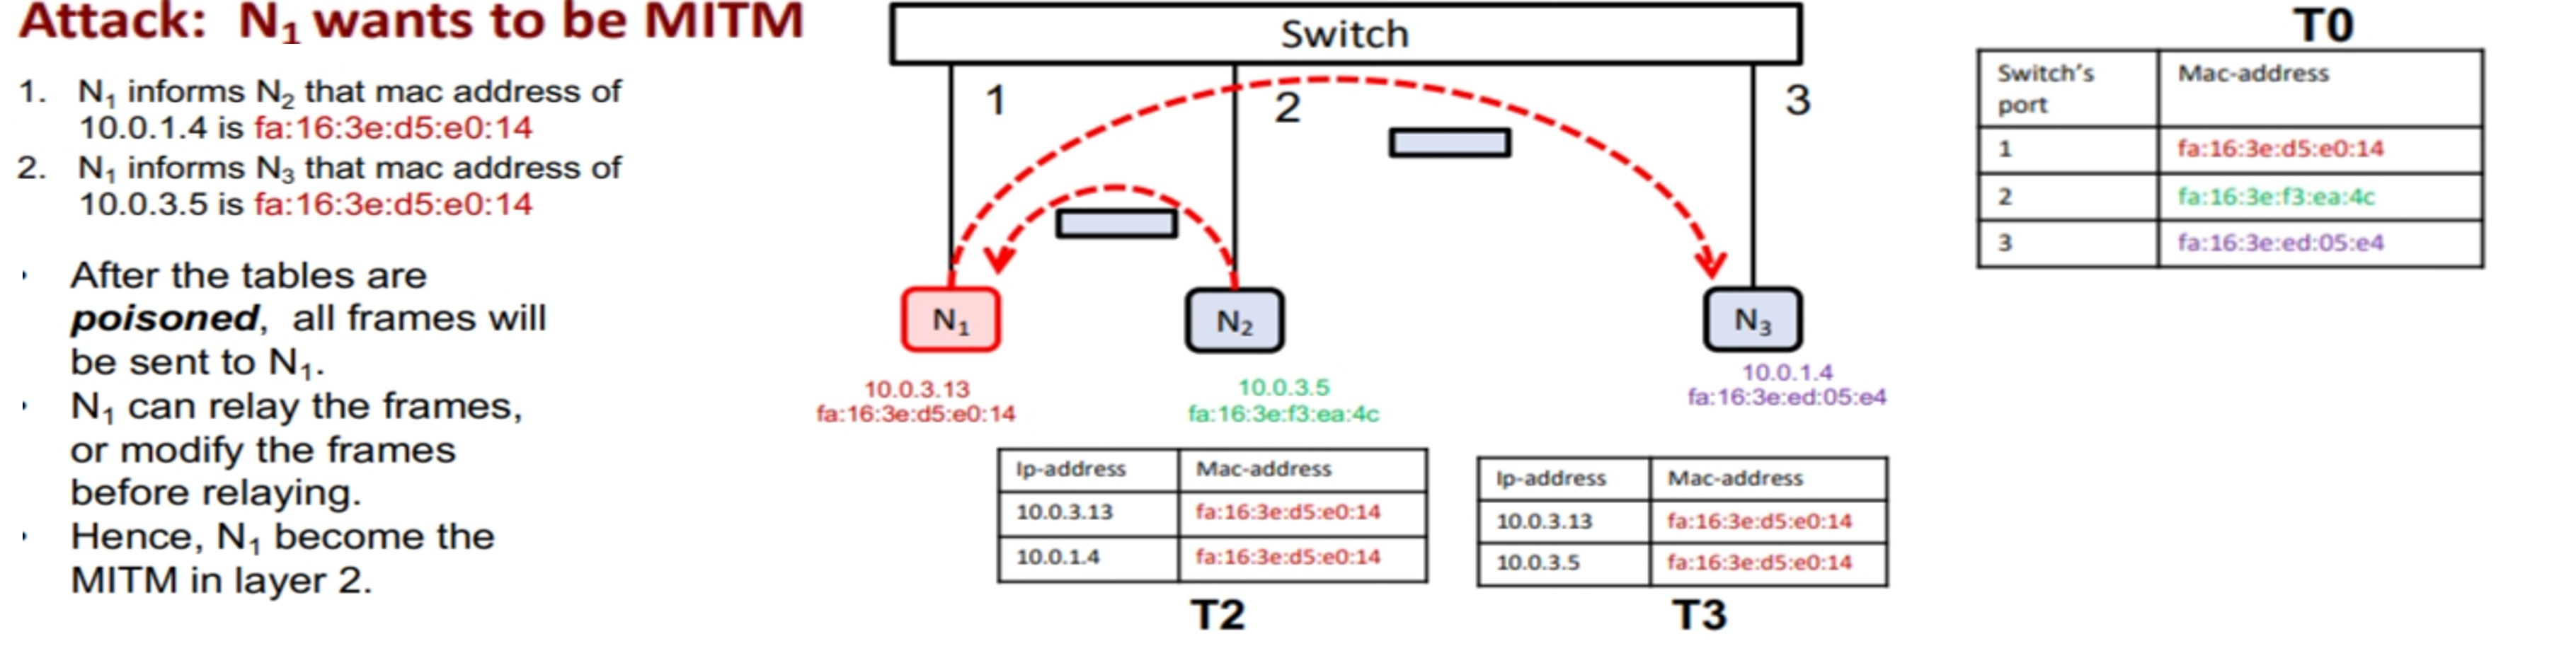
\includegraphics[width=1\linewidth]{ARPPoisoning}}


\section{5.3 Denial of Service Attack}
DoS attacks target \textbf{availability}, preventing some service from being accessible and usable 
upon demand by an authorised entity, delaying time-critical operations. Many successful DOS attacks simply flood the victims with overwhelming requests/data. When DOS carried out by large number of attackers, \textbf{DDOS: Distributed Denial of Service}.

\subsection{Reflection and Amplification attack}
\begin{itemize}
\item \textbf{Reflection}: Reflection attack type of DOS where attackers send requests to intermediate nodes, 
which in turn send overwhelming traffic to the victim. 
\item Indirect, more difficult to trace. 
\item \textbf{Amplification}: Refection attack mechanism can be measured by its amplification factor, which is the size of traffic 
the victim received over the size of traffic sent by the attacker.
\item A single request could trigger multiple responses from the intermediate nodes. Reflection attack aka amplification attack.
\end{itemize}
\centerline{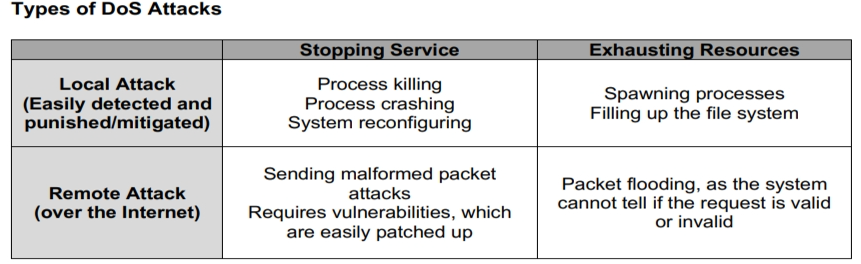
\includegraphics[width=1\linewidth]{DoSAttacks}}

\subsubsection{DoS Example 1: ICMP/Smurf Flood Attack}
“smurf”: Attack can bring down big targets. Attack makes use of public servers to target a specific victim IP address. This 
is done via: \\ \smallskip
1. An attacker sends the “ICMP PING” request to router, instructing router to broadcast request. \\
2. The request’s source IP address spoofed, replaced with victim IP address. \\
3. The router thus broadcasts this request. \\
4. Every entity that receives request replies, sends “Echo reply” to source, which is the victim. \\
5. The victim is overwhelmed with “Echo reply”s from the entire network. \\
6. The attacker thus takes advantage of the amplification effect to attack the victim.
\begin{itemize}
\item Attack no longer effective, as most routers are now configured to not broadcast the requests. To prevent this attack, the measure is to simply disable a feature that was previously thought to be useful.
\end{itemize}

\subsubsection{DoS Example 2: Application-Layer DoS Attack (HTTP Get)}
The trick is to simply flood a web server with HTTP requests. Effective if large number of attackers, since each attacker can only send requests at a low rate. Distributed Denial of Service (DDoS).
\begin{itemize}
\item DDoS is normally achieved via a \textbf{botnet}.
\item A bot, or zombie, is a compromised machine, and a botnet, or zombie army, is a large collection of connected bots, communicating via covert channels.
\item \textbf{Covert channels}: to prevent the owner of the zombie computer from noticing. Owners unaware system used.
\item \textbf{A botnet has a command-and-control mechanism}, can be controlled by a single individual to carry out a Distributed Denial of Service attack.
\item \textbf{Other Botnet Usages}: Vulnerability Scanning, Anonymising HTTP Proxy, Email Address Harvesting, Cipher Breaking etc.
\end{itemize}

\section{5.4 Useful Tools}
\subsection{Wireshark (packets analyzer)}
Wireshark is a popular, free and open-source network packet analyser. It generally performs capturing at the 
link layer. This depends on the operating system and hardware, however. It essentially captures “interactions” 
between the operating system and the network card driver.
\\ \smallskip
Some things that Wireshark can do: View list of packets, View packet details, View packet bytes, Filter for packets, Follow TCP stream.

\subsection{Nmap (Port Scanner)}
A port helps a server decide which application process to handle an incoming packet. By saying that a process or service is “listening” to a particular port, we mean that the process is running and ready to process packets with that particular port number. We also say a port 
is “open” when there exists such a process running in the server. 
\begin{itemize}
\item \textbf{Port scanning}: process of determining which ports are open on hosts in a network.
\item \textbf{Port scanner}: tool to perform port scanning. Useful for both attackers and 
network administrators to scan for vulnerabilities. Nmap is a very popular port scanner.
\item \textbf{Nmap} is a full featured port-scanning tool: Command-line tool with a GUI frontend.
\item Installation: sudo apt-get install nmap, zenmap 
\item Usage: nmap [ScanType(s)] [Options] \{target specification\}
\item Examples: TCP ACK scan (a stealthier scan): nmap -sA, OS fingerprinting: nmap -O, Service/version detection: nmap -sV.
\end{itemize}

\centerline{\includegraphics[width=1\linewidth]{portNumbers}}

\section{5.5 Network Protection: Cryptography}
There are several cryptographic techniques that can help us achieve confidentiality (via encryption) and authenticity (via MAC, PKI, and Strong Authentication) over a public communication channel, even if the adversary can sniff and spoof the data.
\\ \smallskip
There are various security protocols that essentially achieve that, but operates at different layers. Some well-known protocols are:
TLS/SSL, WIFI Protected Access II (WPA2), Internet Protocol Security (IPsec). 

\subsubsection{Note: Discussion of Security protocols and attacks}
Security protocol considers the layer it aims to protect. 
\begin{itemize}
\item \textbf{Complication}: Some protections span across multiple layers, or do not provide full protection of the targeted layer.
\item When analysing an attack, insightful to figure out at which layer the attacker resides or if attacks span across multiple layers. Hard to pinpoint the layer.
\item \textbf{General Guideline}: A security protocol that protects layer k would protect information from that layer and above 
against an attacker sitting at layer k-1 and below.
\item E.g. if attacker resides at layer 1, security protocol protects layer 3. Security protocol protects information generated in layer 3 and 
above, but not the information generated in layer 2.
\end{itemize}

\subsection{5.5.1 Secure Sockets Layer / Transport Layer Security (SSL/TLS)}
The SSL/TLS sits on top of the transport layer. Application passes data, destination IP address to SSL/TLS. SSL/TLS protects the data using encryption (for confidentiality) and MAC (for authenticity), instructs transport layer to send protected data. 
\begin{itemize}
\item \textbf{End-to-end Encryption}: End-to-end encryption performed. Data stays encrypted from one end of its journey to the other.
\item \textbf{Link Encryption / Hop-by-Hop Encryption}. Encryption occurs at the Data Link and Physical layers, and the packet is decrypted at every device between the two ends.
\end{itemize}

\subsubsection{Attack Scenario 1: Attacker at the Physical Layer}
Suppose attacker at physical layer, can sniff/spoof message at layer. Alice uploads her report in café using free and open WIFI, \textbf{no WPA} protection. Anyone in café has access to physical layer. 
\begin{itemize}
\item \textbf{Cannot learn application data}: protected by SSL/TLS in application layer, protected from attacker in lower layers
\item \textbf{Can learn website IP address}: IP headers from network layer, not protected by TLS/SSL (on transport layer) from attacker below at data link/physical layer.
\end{itemize}

\subsubsection{Attack Scenario 2: Attacker at the Application Layer}
Adversary at the application layer. E.g. malicious JavaScript code injected into LumiNUS, executed by Alice’s computer. 
\begin{itemize}
\item \textbf{Can learn/spoof application data}: SSL/TLS cannot protect info from attacker at its layer and above layer. 
\item \textbf{Cannot learn website IP address}: MAC address defined at layer 2. Attacker at application 
layer unable to attack “downwards”, only can attack upwards.
\end{itemize}
\centerline{\includegraphics[width=1\linewidth]{TLSSSL}}

\subsection{5.5.2 WIFI Protected Access II (WPA2)}
WPA2: popular protocol, common in home WIFI access points, more secure than Wired Equivalent Privacy (WEP) (broken), and WPA. Provides protection at layer 2 (Link) and layer 1 (Physical). However, not all information in layer 2 are protected.

\subsubsection{Attack Scenario: Attacker at the Physical Layer}
Attacker at the physical layer who is able to sniff and spoof information, and Alice uploads a report. 
\begin{itemize}
\item \textbf{Cannot learn application data / website IP address}: Data from the upper layers have been encrypted with AES.
\item \textbf{Can learn MAC address}: MAC addresses assigned in the link layer, and is never encrypted.
\end{itemize}
Anyone within the range of network might see traffic, but scrambled with up-to-date encryption standards. WPA2 uses AES and keys that 
are 64 hexadecimal digits long. WPA3 was announced in January 2018.

\subsection{5.5.3 Internet Protocol Security (IPsec)}
IPsec provides \textbf{integrity and authenticity} protection of IP addresses, but not confidentiality. Attackers unable to “spoof” source IP 
addresses, but can learn source and destination IP addresses of sniffed packets. Mechanism whose goal is to protect the IP layer. \\ \smallskip
IPsec is a is a protocol suite for securing Internet Protocol (IP) communications by \textbf{authenticating and encrypting each IP packet of a communication session}. IPsec includes protocols for establishing mutual authentication between agents at the beginning of the session and negotiation of cryptographic keys to be used during the session. 

\begin{itemize}
\item Used in protecting data flows between a pair of hosts (host-to-host), between a pair of security gateways (network to-network), or between a security gateway.
\item Uses cryptographic security services to protect communications over Internet Protocol (IP) networks.
\item Supports network-level peer authentication, data origin authentication, data integrity, data confidentiality (encryption), and 
replay protection. 
\end{itemize}
IPsec is an end-to-end security scheme operating in the Internet Layer of the Internet Protocol Suite, while some other Internet security systems in widespread use, such as Transport Layer Security (TLS) and Secure Shell (SSH), operate in the upper layers at
Application layer. Hence, only IPsec protects any application traffic over an IP network. Applications can be automatically secured by IPsec at the IP layer.

\subsection{Which Layer to Protect?}
Seems protecting lowest layer, can protect information in all layer. However, not feasible as intermediate node needs to access some higher layer info, e.g. ip-address, and sit in higher layer. Hence, a malicious intermediate node could be a MITM in higher layer.
\begin{itemize}
\item Typical implementation use TLS/SSL + WPA2.
\item IPSEC most expensive to implement, difficult to deploy. (“touches” OS).
\end{itemize}


\section{5.6 Network Protection: Firewall, Intrusion Detection System}
SSL/TLS, WPA2 insufficient to protect network. DoS attacks cannot be prevented. Does not protect interactions with many services and applications (e.g. DNS server). Not practical, due to efficiency, to establish a SSL/TLS to the DNS 
server for a DNS query, susceptible to DNS spoofing. \textbf{Need to control the flow of traffic} between networks, especially between the untrusted public network (Internet) and the trusted internal network.
\begin{itemize}
\item \textbf{Principle of Least Privilege PoLP}: requires that in a particular abstraction layer of a computing 
environment, every module (e.g. process/ user/program) must be able to access only the information and resources that are necessary for its legitimate purpose. (adopted in domains of security)
\item Need to divide computer network into segments and deny unnecessary access. 
\item Firewall, IDS are tools to control network access.
\end{itemize}

\subsection{5.6.1 Firewall}
\textbf{A firewall}: device/program, controls flow of network traffic between networks or 
hosts that employ differing security postures. It sits at the border between networks and 
looks at addresses, services and other characteristics of traffic. It then controls what traffic is 
allowed to enter the network (ingress filtering), or leave the network (egress filtering).
\begin{itemize}
\item \textbf{ DMZ: Demilitarized Zone}. A sub-network that exposes the organization’s external 
service to the (untrusted) Internet.
\item Adds additional layer of security, an external network node can access only what is exposed in the DMZ, 
while the rest of the organization's network is firewalled.
\item \textbf{2-firewall Setting}: The first firewall ("front-end" or "perimeter" firewall) configured to allow traffic 
destined to the DMZ only. The second firewall ("back-end" or "internal" firewall) only allows traffic to the DMZ from the internal network.
\end{itemize}

\subsubsection{Packet Filtering/Screening}
Firewall’s controls are achieved by “packets filtering” (aka screening). Filtering may occur in router, gateway/bridge, host, etc. Packet filtering inspects every packet, typically only on the TCP/IP packet’s header information (network \& transport layer). If the payload is inspected, we call it \textbf{deep packet inspection (DPI)}. Action taken after inspection could be to allow packet to pass, drop packet, reject packet (inform sender), log info, notify system admin, modify packet.

\begin{itemize}
\item \textbf{Example Firewall Rules}: 
\item Drop packets with “source ip-address” not within the organization’s network. (To 
stop attacks originated within the network).
\item Whitelist: Drop all packets except those specified in the white-list. (e.g. drop all except http, email 
protocol, and DNS)
\item Blacklist: Accept all packets except those specified in the black-list. (e.g. allow https except ip-address in 
the blacklist)
\end{itemize}

\subsubsection{Firewall Design}
A firewall enforces a set of rules provided by the network administrator. 
An example of rules for Firewall-2 (back-end firewall) would be:
\begin{itemize}
\item Block HTTP
\item Allow from Internal Network to Mail Server: SMTP, POP3
\end{itemize}
An example of rules for Firewall-1 (front-end firewall) would be:
\begin{itemize}
\item Allow from anywhere to Mail Server: SMTP only
\end{itemize}
How the rules are to be specified thus differs based on the devices and software. For a firewall configuration, the table is processed in a top-down manner, and the first matching rule determines the action taken. Hence, the most specific rule is on top, and the most general rule is last.


\centerline{\includegraphics[width=1\linewidth]{firewall}}


\subsubsection{Types of Firewall}
There are 6 types of firewalls in the textbook, but they are usually grouped into 3 types.
\begin{enumerate}
\item \textbf{(Traditional) Packet Filters}: Filters packets based on information in packet headers.
\item \textbf{Stateful-Inspection (Packet Filters)}: Maintains a state table of all active connections, and filters packets based on active connection states.
\item \textbf{Application Proxy}: Understands application logic and acts as a relay of application-level traffic
\end{enumerate}


\subsection{5.6.2 Intrusion Detection System}
An IDS system consists of a set of “sensors” who gather data. Sensors could be in the host, or network router. The data are analyzed for intrusion. Popular open-source IDS: Snort.

\subsubsection{Three types of IDS:}
\begin{itemize}
\item \textbf{Attack signature Detection}: The attack has specific, well-defined signature. For e.g. using certain port 
number, certain source ip address. 
\item \textbf{Anomaly Detection}:  The IDS attempt to detect abnormal pattern. For e.g. a sudden surge of 
packets with certain port number.
\item \textbf{Behavior-based IDS}:  Can be viewed as a type of anomaly detection that focuses on human 
behavior. For e.g. The system might keep the profile of each user. It then tries to detect any user who deviates from the profile (e.g. start to download large files).
\end{itemize}






\section{5.7 Network Security Management}
There is a need to continuously monitor and adjust network characteristics. Best Practices:
\begin{itemize}
\item \textbf{Security Operations Center (SOC)}: Centralised unit in an organisation that monitors the IT systems and deals with security 
issues.
\item \textbf{Security Information and Event Management (SIEM)} “SIM”: Approach that aims to provide real-time analysis of 
security alerts generated by network hardware and network applications. May include capabilities of Data aggregation and correlation, - Event alerting, Compliance report generation, Forensic analysis.
\end{itemize}

\vfill \null
\columnbreak

\vfill \null
\columnbreak

\section{6. Software Security}
Requirements of a program: \textbf{Correct, efficient, secure}. However, program sometimes behaves beyond intended functionality.
\begin{itemize}
\item \textbf{Security Problems faced}: Insecure implementation, unanticipated input. (Use program to elevate privilege).
\item \textbf{Examples}: Buffer overflow, SQL injection, Integer Overflow.
\item \textbf{Root Causes}: Security as secondary goal, unavoidable mistakes, complex modern OS etc.
\end{itemize}

\section{6a. Call Stack}
Concepts in software security require strong understanding on runtime environment of a piece of code.

\begin{itemize}
\item Process integrity can be compromised by modifying values in memory. 
\item Call stack facilitates function calls. It keeps track of different instances of function call. Without 
that, we won’t have modular software design. 
\item “Stack frames” contains info of function environment, including control flow info (return address), local variables, parameters. Malicious modification has significant consequence (stack smash + buffer overflow).
\end{itemize}

\subsection{6a.1 Computer Architecture}
\subsubsection{Code vs. Data}
Modern computers are based on the Von Neumann computer architecture. 
\begin{itemize}
\item Code treated as data, both stored in same memory. No clear distinction of code and data. (Compared to Harvard architecture). 
\end{itemize}
\textbf{Attack: Programs may be tricked into treating input data as code} (code-injection attacks)

\subsubsection{6a. 2Program Control Flow}
\begin{itemize}
\item \textbf{Control Flow}: Program counter register holds memory address of next instruction to be executed.
\item Program counter can be incremented, do direct jump (constant value address), indirect jump (address value fetch from memory).
\item \textbf{Control Flow Integrity}: If attack can modify some memory, can compromise execution integrity (modify code or address in indirect branch).
\end{itemize}
\textbf{Memory Integrity:} Not easy for attacker to compromise memory integrity. May exploit some vulnerabilities to “trick” victim process to write to memory locations, e.g. via a buffer overflow attack. Has restrictions: (only writeable to small amount of memory / sequence of consecutive bytes). Attack needs to be very precise and surgical. \\
\textbf{Possible Attack Mechanisms}: Overwrite existing execution code portion with malicious code; or overwrite a piece of control-flow information. (Replace memory location storing a code address for direct jump / indirect jump).

\subsubsection{6a.3 Functions, Stack (Execution Stack, Call Stack)}
Functions manage their "runtime environment" (local var, arguments) using "call stack".
\begin{itemize}
\item Stack is a data structure, call-stack stores information of function calls. Stack pointer is variable storing location of first element. 
\end{itemize}
\textbf{Security Implication}: Using buffer overflow (next week), attacker could modify the stack (stack smash). Stack smash has two effects: If return address is modified, the control flow is compromised. If local variables are modified, the computed result would be wrong.

\section{6b. Secure Programming}
Well known reference: \textbf{24 Deadly Sins of Software Security: Programming Flaws and How to Fix Them. McGraw-Hill, 2010.}:  Buffer Overruns, Format String Problems, Integer Overflows, SQL Injection, Errors Handling, Race Conditions, Trusting Network Address Resolution (ARP), etc.

\section{Attacks and Vulnerabilities}

\subsection{6b.1 Printf() and Format String Vulnerability}
Uncontrolled format string (type of code injection vulnerability). Discovered around 1989, used in security exploits.
\begin{itemize}
\item Format string exploits can crash program or execute harmful code. Unchecked user input as format string parameter such as C printf().
\item \textbf{Exploitation}: attacker might be able to (1) obtain more information (confidentiality), (2) cause program to crash, e.g. using \%s, \%x. (execution integrity), (3) modify memory content using “\%n”. (memory integrity, lead to execution integrity)
\end{itemize}
\textbf{Example:} printf() explotable if format specifier within, searchs for second parameter in the stack to be displayed. When supplied by
user, can get information by designing string to be printed.
\begin{itemize}
\item If program has elevated privilege (set UID enabled), attacker might obtain information previously inaccessible.
\item \textbf{Simple Prevention Measure}: Avoid taking a user input as a format string. We can read the input into a separate variable, 
then print out that variable via our own format string. 
\end{itemize}

\subsection{6b.2 Data Representation}
Different parts of a program or system may adopt different data representations. Such inconsistencies could lead to vulnerabilities.
\begin{itemize}
\item For example, CVE-2013-4073: “Ruby’s SSL client implements hostname identity check, but 
it does not properly handle hostnames in the certificate that contain null bytes.”
\end{itemize}
\textbf{String representation}: In C, null character indicates end of string. However, not all systems adopt such convention. Here, we separate as two types for discussion: \textit{NULL/Non-Null-termination representation.}

\subsubsection{Exploit Vulnerability 1: NULL-Byte Injection}
A CA may accept hostname containing a null character, e.g. nus.edu.sg$\backslash$0.attacker.com. Vulnerable verifier might use both representation to verify certificate. (verifies certificate based on non-NULL-termination, compare name in certificate / name entered by user based on NULL-termination representation)
\begin{itemize}
\item \textbf{Example Attack}: Attacker register domain name, purchase valid certificate from a CA.  (*.attacker.com). Set up spoofed website of NUS with domain name (nus.edu.sg$\backslash$0.attacker.com). 
\item Attacker direct victim to spoofed webserver (E.g., phishing email, evil café owner). Attacker’s webserver presented the certificate C1, browser displays address (based on null-termination) on browser’s address bar. 
\item Browser verified the certificate (based on non null-termination). Since valid, browser displayed pad-lock in the address bar.
\end{itemize}
\centerline{\includegraphics[width=0.8\linewidth]{nullByteAddress}}

\subsubsection{Exploit Vulnerability 2: UTF-8 “Variant” Encoding Issues}
Many implementations accept multiple and longer “variants” of a character. Leads to certain issues.
\begin{itemize}
\item \textbf{File Access Containment}: Could be compromised. Using different variants of inputs can bypass blacklisted inputs, which when decoded give same system call to access some file at another directory point.
\item \textbf{IP Address}: For e.g. 4 byte IP written as string, checked against blacklist, and parsed, then calculated to form back 32 bit integer. Process can be exploited, as integers can go negative. Unexpected and undesired results may occur. 
\end{itemize}
\textbf{Preventive Measures:} Data Representation issues: Use Canonical Representation. Cannot trust input from the user, do not directly 
use input. Always convert input to standard i.e. canonical representation immediately. Preferably, do not rely on verification check done in the application. Make use of the underlying system access control mechanism.

\subsection{6b.3 Buffer Overflow}
In languages such as C and C++, programmers manage the memory via pointer arithmetic. No array-bound checking. Such flexibility is useful but prone to bugs, leading to vulnerabilities.

\subsubsection{Example: C function strcpy prone to buffer overflow}
\centerline{\includegraphics[width=0.8\linewidth]{strcpy}}
In above, length of s2 potentially more than 10, as length determined by first occurrence of null. The strcpy() may copy the whole string of s2 to s1, even if length of s2 is more than 10. Since buffer size of s1 only 10, extra values overflowed, written to other parts of the memory.
\begin{itemize}
\item If s2 supplied by malicious user, well-crafted input can overwrite important memory and modify the computation.
\item \textbf{Preventive Measure}: Use strncpy(s1, s2, n) instead, at most $n$ characters copy. However, still exploitable with improper usage.
\end{itemize}

\subsubsection{Stack Smashing}
Stack smash is a special case of buffer overflow that targets stack. Buffer overflow on
stack is called stack overflow, stack overrun, or stack smashing.
\begin{itemize}
\item If stack buffer filled with data supplied from untrusted user, can corrupt the stack to inject executable code and take control of process. Oldest and one of more reliable methods for attackers to gain unauthorized access to a computer.
\item Well-designed overflow could also inject the attacker’s shellcode into the process’ memory, then execute the shellcode. If the target executable is set-UID-root, then the injected shellcode runs with root privilege.
\item Some defences such as canary are available.
\end{itemize}


\subsection{6b.4 Integer Overflow}
The integer arithmetic in many programming languages is actually modulo arithmetic. Suppose a is a single byte (i.e. 8-bit) unsigned integer.
\centerline{$a = 254$}
\centerline{$a = a+2$}
Its value would now be 0, since the addition is done in the form of modulo 256. Hence, the 
predicate (a < a+1) is not always true! Many programmers do not realise this, leading to 
possible vulnerabilities.

\subsection{6b.5 Code Injection}
Many attacks inject malicious codes as data. Scripting languages vulnerable to such attack. \textbf{Script programs} automate execution of tasks that could alternatively be executed line-by-line by a human operator. \\
Scripting language typically “interpreted”, instead of compiled. (E.g. PHP, Perl, JavaSript, SQL.)
\begin{itemize}
\item Many scripting languages allow “script” to be data storing in variables. This opens up the
possibility of injecting malicious code into the script.
\end{itemize}

\subsubsection{SQL injection}
For e.g. a script first gets the user’s input and stores it in the variable \$userinput. Next, it runs the following:
\centerline{SELECT * FROM client WHERE name = ‘\$userinput`}
Attacker not knowing any name can set \$userinput as: anything’ OR 1=1 --. (-- marks start of comment). Then, all records will be displayed.

\subsection{6b.6 Undocumented Access Point}
For debugging purposes, many programmers insert undocumented access points to allow them to better inspect states. 
\begin{itemize}
\item E.g. press certain combo of keys displays certain variables 
\item Certain input strings cause the program to branch to some debugging mode
\item Access points left in final production system, providing backdoors. 
\end{itemize}
A \textbf{backdoor} is a covert method of bypassing normal authentication. (Aka Easter eggs). Some benign, intentionally planted for fun). However, known cases of unhappy programmers plant backdoors on purpose, accessible to any other user who knows / discovers them.


\subsection{6b.7 TOCTOU}
\textbf{Time-of-Check Time-of-Use} (TOCTOU) Race Condition: Race condition occurs when multiple processes access a piece of shared data, final outcome depends on the sequence of the accesses.
\begin{itemize}
\item A vulnerable process A that checks for permission to access a shared data, subsequently accesses the data.
\item A malicious process B that swaps the data.
\end{itemize}
Two processes run by single malicious user in system. Race between processes A and B. If B completes swapping after A checks for permission but before A accesses the data, attack succeeds.
\centerline{\includegraphics[width=0.8\linewidth]{TOCTOU}}
\begin{itemize}
\item \textbf{Preventive Measure}: Avoid writing own access-control on files, let OS do it by setting process credentials. E.g. set process’ effective UID to user real UID (normal/non-root) before accessing the file. OS checks permission, decides to grant or deny access. After, reset effective UID back to root if required.
\item \textbf{See CWE-367 (Common Weakness Enumeration)}: (use symbolic link to point to sensitive system file.)
\item \textbf{Preventive Measure}: In C programming, avoid using separate system calls that take the same filename as input. 
Instead, try to open the file only once, effectively locking it to block any further changes by other processes, and use the file handle/descriptor. 
\end{itemize}



\section{6c. Defence and Preventive Measures}
Many bugs and vulnerabilities are due to a programmer’s ignorance. Difficult to ensure that a program is bug-free. However, there are various useful countermeasures available.

\subsection{6c1. Filtering (input validation)}
Many attacks carried out by feeding carefully-crafted input to the system. Inputs do not follow the expected format, e.g. 
input is too long, contains control or meta characters, contains negative numbers etc. Use input validation or filtering whenever an 
input is required from the user. (Implement in web server / SQL server. but not at browser level).
\begin{itemize}
\item \textbf{Approach}: Use whitelist or blacklist.
\item \textbf{Difficulties}: Difficult to ensure filtering is perfect and complete, (e.g. UTF-8). Very hard to design.
\end{itemize}

\subsection{6c2. Use safer functions}
Completely avoid functions that are known to create problems. Use the “safe” version of the functions. However, even if they are avoided, there could still be vulnerability. 

\subsection{6c3. Bound check and “Type” Safety}
\textbf{Bound Check}: Some programming languages (Java, Pascal) perform bounds checking at runtime. When array declared, upper and lower bounds have to be declared. When reference to array location made, checked against bounds, if checks fail, halted, throw exception. Reduce efficiency, prevent buffer overflow. (C, C++ do not perform bound checking). \\

\textbf{Type Safety}: Some p. languages carry out type checking, ensure arguments operation get during execution are always correct. For example, trying to do a = b; when a is an 8-bit integer and b is a 64-bit integer would throw an error.

\subsection{6c4. Protecting the memory (randomization, canaries)}
\textbf{Randomization}: Attackers gain when data and codes stored in same locations in memory. Address space layout randomization (ASLR) as prevention technique, decrease attacker’s chances. ASLR randomly arranges the address space positions of key data areas of a process, including the base of the executable and the positions of the stack, heap and libraries. Use \{sudo sysctl -w kernel.randomize\_va\_space=0\} to turn disable ASLR in Linux. \\

\textbf{Canaries}: secret values inserted at selected memory locations during runtime. If modified at runtime (checked), program halts.  Help detect (but not prevent) buffer overflow, especially stack overflow. In typical buffer overflow, consecutive memory locations have to be ran over. The canaries naturally modified. \\

Keep values secret. If attacker knows, simply write to canary while overrunning, impossible to detect. In Linux, turn off gcc canary-based stack protection by supplying flag when compiling: \{-fno-stack-protector\}

\subsection{6c5. Code Inspection (taint analysis)}
\textbf{Manual Checking}: tedious.\\
\textbf{Automated Checking}: Some automations possible. \\
\textbf{Taint analysis}: Input from users are source. Critical functions are sinks. Check if sink’s arguments affectable (i.e. tainted) by source. If yes, special check (e.g. manual inspection) carried out. Can be static analysis (check code without “tracing it”), or dynamic (i.e. run code with some input). (E.g. Sinks: opening of system files, function evaluating SQL command, etc.)

\subsection{6c6. Testing}
\textbf{Vulnerabilities} can be discovered via testing. There are three types of testing: White-box testing (access to application’s source code), Black-box testing (no access), Grey-box testing (combination, tester reverse-engineered binary or executable). \\
Security testing attempts to discover areas susceptible to intentional attack, and hence would test for inputs that rarely occur under normal circumstances, e.g. very long names, names with numeric values, strings containing meta characters, etc. \\
\textbf{Fuzzing} is technique that sends malformed inputs to discover vulnerabilities. Fuzzing can be both automated or semi-automated, and is more effective than simply sending in random inputs.

\subsection{6c7. The principle of Least Privilege}
When writing a program, be conservative in elevating privileges. When deploying a software system, do not give users more access 
rights than necessary, and do not activate unnecessary options. (E.g. web-cam software with remote control it. Features by default switched off when shipped clients?) \\
\textbf{Hardening}: process of securing a system by reducing surface of vulnerability. Done by reducing number of functions in a system.


\subsection{6c8. Keeping up to date (Patching)}
Lifecycle of vulnerability: discovered $\rightarrow$ affected code fixed $\rightarrow$  tested $\rightarrow$ patch made public $\rightarrow$
patch is applied. \\
In some cases, vulnerability announced without technical details before patch is released. Likely only known to small number of attackers, 
or even none, before it is announced. When patch is released, may actually help attackers to derive the vulnerability, by inspecting patch. Number of successful attacks can go up after vulnerability/patch announced, more attackers aware of exploit. \\
\textbf{Crucial to apply patch timely}: Much more complex than it seems: for critical systems, it is not wise to apply the patch immediately before rigorous testing. (E.g. may cause train scheduling software to crash, affect operations of organisations).

\subsection{6c Summary}
Defence mechanisms and countermeasures, to be adopted at different stages of the Software Development Lifecycle (SDLC):
\begin{itemize}
\item \textbf{Development Stage}: Safer Functions, Bounds Checking and Type Safety, Filtering (Input validation), Code Inspection (Taint analysis), Principle of Least Privilege, Enabled Memory Protection.
\item \textbf{Testing Stage}: Fuzzing and Penetration Testing
\item \textbf{Deployment (including Software Execution) Stage}: Runtime Memory Protection*, Randomization, Principle of Least Privilege*: Disable Unnecessary Features, Patching.
\end{itemize}



\vfill \null
\columnbreak

%% COMMENT OUT
\fi

\section{7. Access Control}
\begin{itemize}
\item \textbf{Access control}: selective restriction of access to place/resource.
\item Access control specified through operation, objects, subjects (principle). Make use of access control matrix to simplify representation. 
\item \textbf{Guidelines}: Security perimeter, security boundary, principle of least privilege, segregation, compartment, segmentation, firewall
\item Sharing info across security perimeter: \textit{bridge, privilege elevation}.
\end{itemize}


\subsection{7.1 Access Control Model}
Structure to specify restrictions on subjects (users), objects and operations (actions).


\subsection{7.2 Access Control Matrix}



\subsection{7.3 Intermediate Control}



\subsection{7.4 Unix}


\subsection{7.5 Elevated Privilege and Controlled Invocation}


\subsection{7.6 Controlled Invocation in Unix}

















\vfill \null
\columnbreak


\section{8. Web Security}















\end{multicols*}
\end{document}
